
% Base de dados. Citar figura \ref{identificador}.

% \begin{figure}[!ht]
% \begin{center}
% \setcaptionmargin{1cm}
% 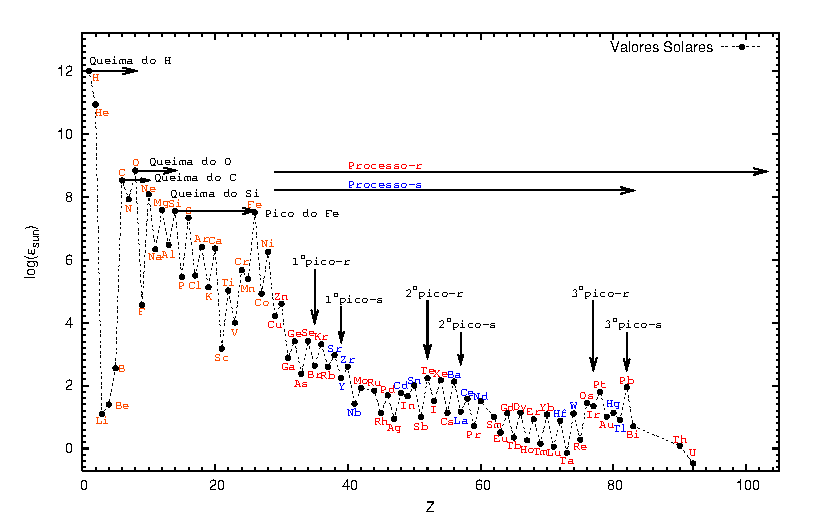
\includegraphics[width=1.0 \columnwidth,angle=0]{fig/solar_grevesse.eps}
% \caption[Resumo da legenda da figura (aparece na lista de figuras)]{Legenda da figura.} 
% \label{identificador}
% \end{center}
% \end{figure}


% \begin{center}
\setcaptionmargin{1cm}
\scriptsize
\begin{longtable}{lcccc}
\caption[Resumo da legenda da tabela (aparece na lista de figuras)]{Exemplo de tabela feita com o longtable.}\\
\hline \hline \\[-2ex]
\multicolumn{1}{c}{Coluna1} &
\multicolumn{1}{c}{Coluna2} &
\multicolumn{1}{c}{Coluna3} &
\multicolumn{1}{c}{Coluna4} &
\multicolumn{1}{c}{Coluna5} 

\\[0.5ex] \hline
\\[-1.8ex]

\endfirsthead

\multicolumn{5}{c}{\footnotesize{{\slshape{{\tablename} \thetable{}}} - Continuação}}\\[0.5ex]

\hline \hline\\[-2ex]

\multicolumn{1}{c}{Coluna1} &
\multicolumn{1}{c}{Coluna2} &
\multicolumn{1}{c}{Coluna3} &
\multicolumn{1}{c}{Coluna4} &
\multicolumn{1}{c}{Coluna5} 

\\[0.5ex] \hline
\\[-1.8ex]

\endhead

\multicolumn{3}{l}{{\footnotesize{Continua na próxima página\ldots}}}\\
\endfoot
\hline

\endlastfoot

1 & 2 & 3 & 4 & 5 \\
6 & 7 & 8 & 9 & 10\\

\label{tabela_com_longtable}
\end{longtable}
\end{center}

\chapter{Theoretical Background}\label{fundamentos}

\section{Cyclones: Categories and Definitions}

For an effective analysis and study, a phenomenon must first be accurately defined. The Glossary of Meteorology by \citet{AMS2023Cyclone} characterizes a "cyclone" as "An atmospheric cyclonic circulation, a closed circulation. A cyclone's direction of rotation (counterclockwise in the Northern Hemisphere) is opposite to that of an anticyclone. (...) Because cyclonic circulation and relative low atmospheric pressure usually coexist, in common practice the terms cyclone and low are used interchangeably. Also, because cyclones are nearly always accompanied by inclement (often destructive) weather, they are frequently referred to simply as storms". This definition categorizes cyclones into sub-types based on their occurrence location: tropical, extratropical, and subtropical cyclones \citep[e.g.]{reboita2017ciclones}. This classification is supported by the assumption that cyclones within the same latitude bands share genesis environments and dynamic maintenance processes. There are also cyclones whose genesis is found in high latitudes, called polar lows \citep[e.g.]{emanuel1989polar,harrold1969polar}. These will not be discussed in depth as the focus of the present study is on the systems generated in the adjacent regions to the South American coast.

The aforementioned definition, while broad, lacks precise criteria. Thus, subsequent sections will employ the Aristotelian approach to elucidate physical phenomena \citep{aristotle1933metaphysics}. Aristotelian causes, foundational to Aristotle's philosophy, offer a comprehensive explanation for an object or phenomenon's existence through four types: material, formal, efficient, and final causes. The ensuing subsections will detail each cause, enhancing the understanding of related phenomena. For each cyclone type — extratropical and tropical — a discussion of the causes will facilitate a direct comparison between the systems.

It is important to note that the structure and mechanisms underlying the genesis and development of cyclones have been well-documented since the mid-twentieth century, leading to the inclusion of many historical references. The aim is to highlight distinctions between cyclone types, a comparison not commonly made in literature. Meteorologists often specialize as "tropical meteorologists" or "mid-latitude meteorologists", a division reflected in educational materials. Some texts focus exclusively on mid-latitude or tropical dynamics \citep[e.g.]{chan2010global,bluestein1992synoptic}, while others that address both, treat them separately \citep[e.g.]{holton1973introduction,donald2015meteorology}. Although this separation is customary and beneficial, juxtaposing the two offers novel insights, as explored in the following sections.


\subsection{Material Causes}\label{material_cause}

Material cause, within the Aristotelian framework, denotes the substance or constituents that form an object. It encompasses the matter or physical elements constituting an entity, serving as the foundation for its existence. For instance, wood acts as the material cause for a table, just as water serves as the material cause for a river. Applied to cyclonic systems, the material cause encompasses the air masses forming these systems, particularly emphasizing their thermal structure. This section elaborates on this concept, showcasing its relevance in defining and categorizing cyclonic systems.

The concept of an air mass, as introduced by Swedish meteorologist Tor Bergeron in 1928, describes a large body of air characterized by uniform temperature, moisture, and other properties, extending over 500 to 5000 km and encompassing the troposphere's full height \citep{stull2015practical}. Air masses are classified based on their temperature, moisture content, stratification, and turbidity levels. Additionally, air masses originate from specific source regions, areas conducive to their formation. The characteristics of an air mass are significantly influenced by its source region's surface conditions, necessitating a flat terrain and mild winds for its development \citep{donald2015meteorology}. Heat transfer between the surface and the air is gradual, requiring the air mass to remain over its source region for an extended period to assimilate its properties \citep{spiridonov2021fundamentals}. Therefore, mid-latitudes, characterized by variable meteorological conditions and strong winds, are generally unsuitable for air mass formation.

Bergeron's classification system is the most widely accepted methodology for categorizing air masses. It utilizes letters to denote the moisture content and the origin of air masses \citep{spiridonov2021fundamentals}. The initial letter signifies the air mass's moisture source—continental (dry) or maritime (moist)—while the subsequent letter indicates the geographical origin of the air mass, whether it be tropical (T), polar (P), arctic/antarctic (A), equatorial (E), or monsoonal (M). Figure \ref{massas_Bergeron} illustrates the spatial distribution of air masses according to Bergeron's scheme. Upon the encounter of two distinct air masses, immediate mixing does not occur, resulting in a temporary discontinuity at their intersection, known as fronts \citep{spiridonov2021fundamentals,donald2015meteorology}.

\begin{figure}[h]
\begin{center}
\setcaptionmargin{1cm}
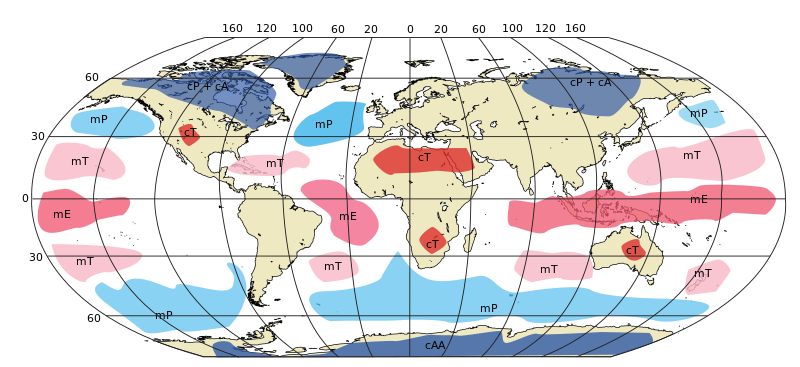
\includegraphics[width=0.7\columnwidth,angle=0]{fig/Air_masses.svg.png}
\caption[Air masses]{Spatial distribution of air masses according to Bergeron's classification. Credit: public domain (https://commons.wikimedia.org/w/index.php?curid=12526643).} 
\label{massas_Bergeron}
\end{center}
\end{figure}

Therefore, the validity of the traditional cyclone classification—tropical, extratropical, and subtropical—relies on the premise that different types of cyclones are initiated by distinct air masses. Specifically, tropical cyclones originate from warm, moist air masses that span the entire troposphere and form over warm tropical waters \citep{gray1968global, frank1977structurea, ramage1959hurricane, riehl1948formation}. In contrast, extratropical cyclones are associated with frontal zones at mid-latitudes, where two different air masses meet, and are typically linked to cold cores \citep{bjerknes1944theory, shapiro1990fronts,hart2003cyclone}. However, intense marine extratropical cyclones can experience warm seclusion, resulting in a warm core at the system's center \citep{hart2003cyclone,shapiro1990fronts}. Subtropical cyclones feature a hybrid structure between tropical and extratropical systems, with warm, moist cores that are less pronounced and shallower than those in tropical cyclones \citep{hart2003cyclone}.

\citet{hart2003cyclone} offers an objective methodology for identifying the thermal structure of cyclonic systems. This analysis focuses solely on tropospheric levels (up to 300 hPa) because cyclones display an opposing thermal signal in the stratosphere. The study examines layers between 900 and 600 hPa and between 600 and 300 hPa, which have comparable masses. Levels below 900 hPa are excluded to prevent extrapolation below the ground or into the boundary layer, which may not accurately represent the cyclone's structure in the free atmosphere. Consequently, the variable corresponding to the cyclonic perturbation in height is defined as follows:

\begin{equation}\label{height_pertubation}
    \Delta Z = Z_{MAX} - Z_{MIN}
\end{equation}

Where \(Z_{MAX}\) and \(Z_{MIN}\) represent the maximum and minimum geopotential heights at a specific isobaric level, measured within a 500 km radius from the cyclone's center. Following this definition:

\begin{equation}
    \Delta Z = \frac{dg |V_g|}{f}
\end{equation}

Here, \(d\) denotes the distance between the geopotential height extremes, \(g\) is the acceleration due to gravity, \(f\) represents the Coriolis parameter, and \(V_g\) is the geostrophic wind speed. Consequently, the cyclone's vertical structure (indicative of a cold or warm core) is determined by the vertical gradient of \(\Delta Z\), which is proportional to the magnitude of the scaled thermal wind (\(V_T\)) for a constant \(d\), applied across two tropospheric layers of equal mass:


\begin{equation}
    \frac{\partial (\Delta Z)}{\partial \ln p} \Bigg|_{600 hPa}^{300 hPa} = -|V^{U}_{T}| \\
\end{equation}
\begin{equation}\label{eq_VTL}
    \frac{\partial (\Delta Z)}{\partial \ln p} \Bigg|_{900 hPa}^{600 hPa} = -|V^{L}_{T}| \\
\end{equation}

where \(V^{U}_{T}\) and \(V^{L}_{T}\) symbolize the thermal winds at upper and lower levels, respectively. As such, positive values of \(-V_T\) signify a warm core within the respective layer, whereas negative values indicate a cold core.

The relationship between the temperature and depth of the core within cyclonic systems is detailed through a phase diagram by \citet{hart2003cyclone}, depicted in Figure \ref{phase_space_Hart_1}. This diagram utilizes the abscissas to represent the parameter \(-V^{L}_{T}\), illustrating the low-level core's thermal structure. The ordinates display \(-V^{U}_{T}\), portraying the high-level core's thermal structure. Integrating these metrics allows for discerning whether a system possesses a warm or cold core, and if it is shallow or deep. Figure \ref{phase_space_Hart_1} includes typical positions representative of different cyclonic types within the phase space. As noted by \citet{hart2003cyclone}, a system may shift within this diagram throughout its lifecycle, making the depiction general for each cyclone category. Additionally, Hart proposes a diagram for the horizontal structure of these systems, related to their formal causes, which is addressed in Section \ref{formal_cause}.

\begin{figure}[h]
\begin{center}
\setcaptionmargin{1cm}
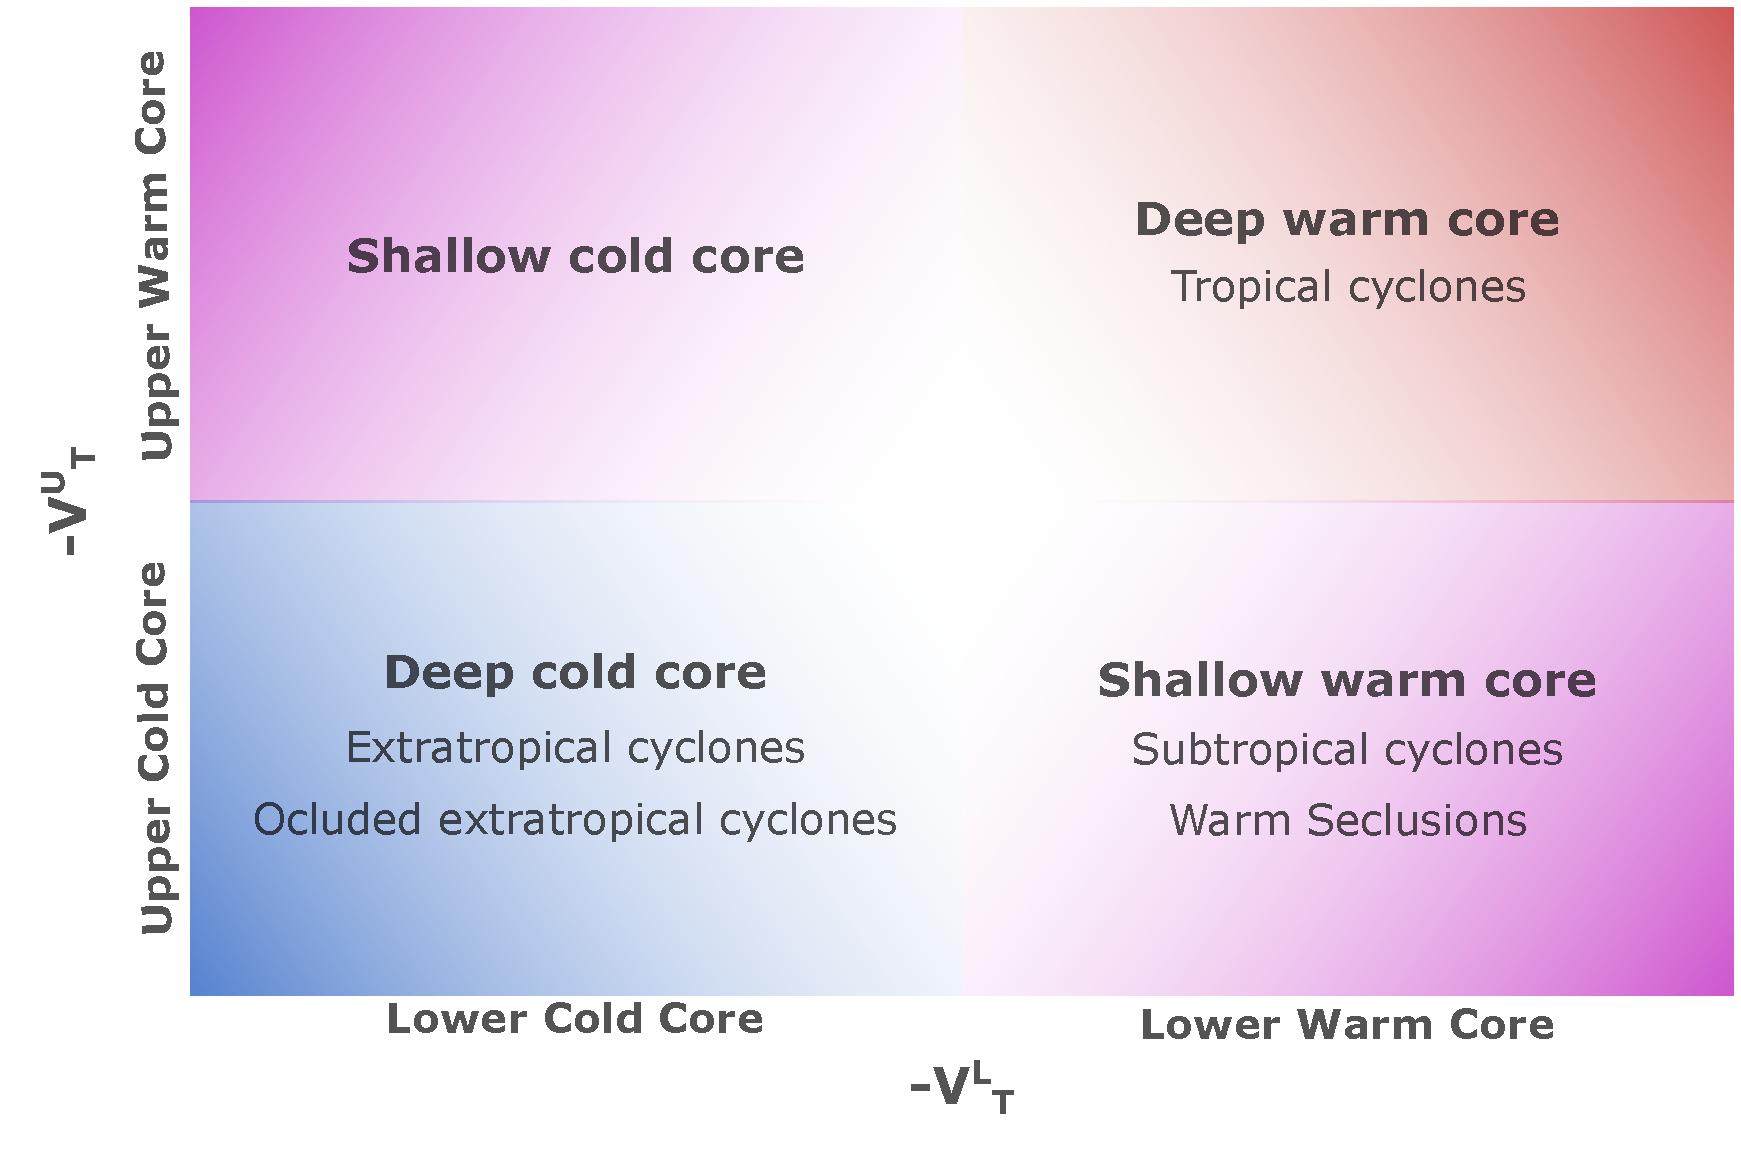
\includegraphics[width=0.7\columnwidth,angle=0]{fig/hart_diagram_1.pdf}
\caption[Phase Diagram - Hart]{Phase diagram showing the relationship between the core temperature of cyclonic systems and their classification. Adapted from \citet{hart2003cyclone}.} 
\label{phase_space_Hart_1}
\end{center}
\end{figure}

Thus, material causes, tied to the thermal structure of cyclonic systems, offer a foundational method for classifying and differentiating cyclone types. This classification leverages the phase diagram by \citet{hart2003cyclone} for an objective categorization. Accordingly, extratropical cyclones are characterized by cold, deep cores, whereas tropical cyclones feature warm, deep cores. This spectrum isn't binary; there exists a gradient of thermal structures with systems exhibiting intermediate features classified as subtropical cyclones. Nevertheless, relying solely on thermal attributes for classification is insufficient. For instance, extratropical cyclones, through the warm seclusion process \citep[e.g.]{shapiro1990fronts}, can develop warm, shallow cores \citep{hart2003cyclone}, indicating the necessity for a broader analysis incorporating additional Aristotelian causes for a comprehensive classification.

\subsection{Formal Causes}\label{formal_cause}

The formal cause concerns the essence or identity that defines a thing, essentially its design, structure, or conceptual blueprint that marks it as a particular type. To revisit the earlier example of a table from Section \ref{material_cause}, its formal cause is the design that qualifies it as a table rather than a chair. In the context of cyclones, the formal cause refers to the system's organizational structure, such as the configuration of convection bands and/or fronts, along with the low-pressure pattern.

Extratropical cyclones, typically associated with mid-latitudes and frontal structures, exhibit an average diameter between 1200 and 1800 km. This size fluctuates over their lifecycle, with the cyclone's diameter expanding by up to 150\% during its intensification phase \citep{simmonds2000size, rudeva2007climatology}. However, the spatial complexity and variability of these systems throughout their lifecycle pose methodological challenges for accurately estimating their dimensions and comparing findings across different studies.

The seminal model describing the formation and horizontal structure of extratropical cyclones was introduced by \citet{bjerknes1919structure}, illustrated in Figure \ref{bjerknes_cyclone}. This model showcases the cyclone's movement along a central horizontal line, with the "steer line" demarcating the boundary that influences the cyclone's trajectory, characterized by warm air masses to its left. The "squall line" indicates a zone of intense meteorological activity, marked by strong winds and often heavy precipitation, with cold air masses located to its left. The "fore runner" represents a region of diverging airflow.

\begin{figure}[h]
\begin{center}
\setcaptionmargin{1cm}
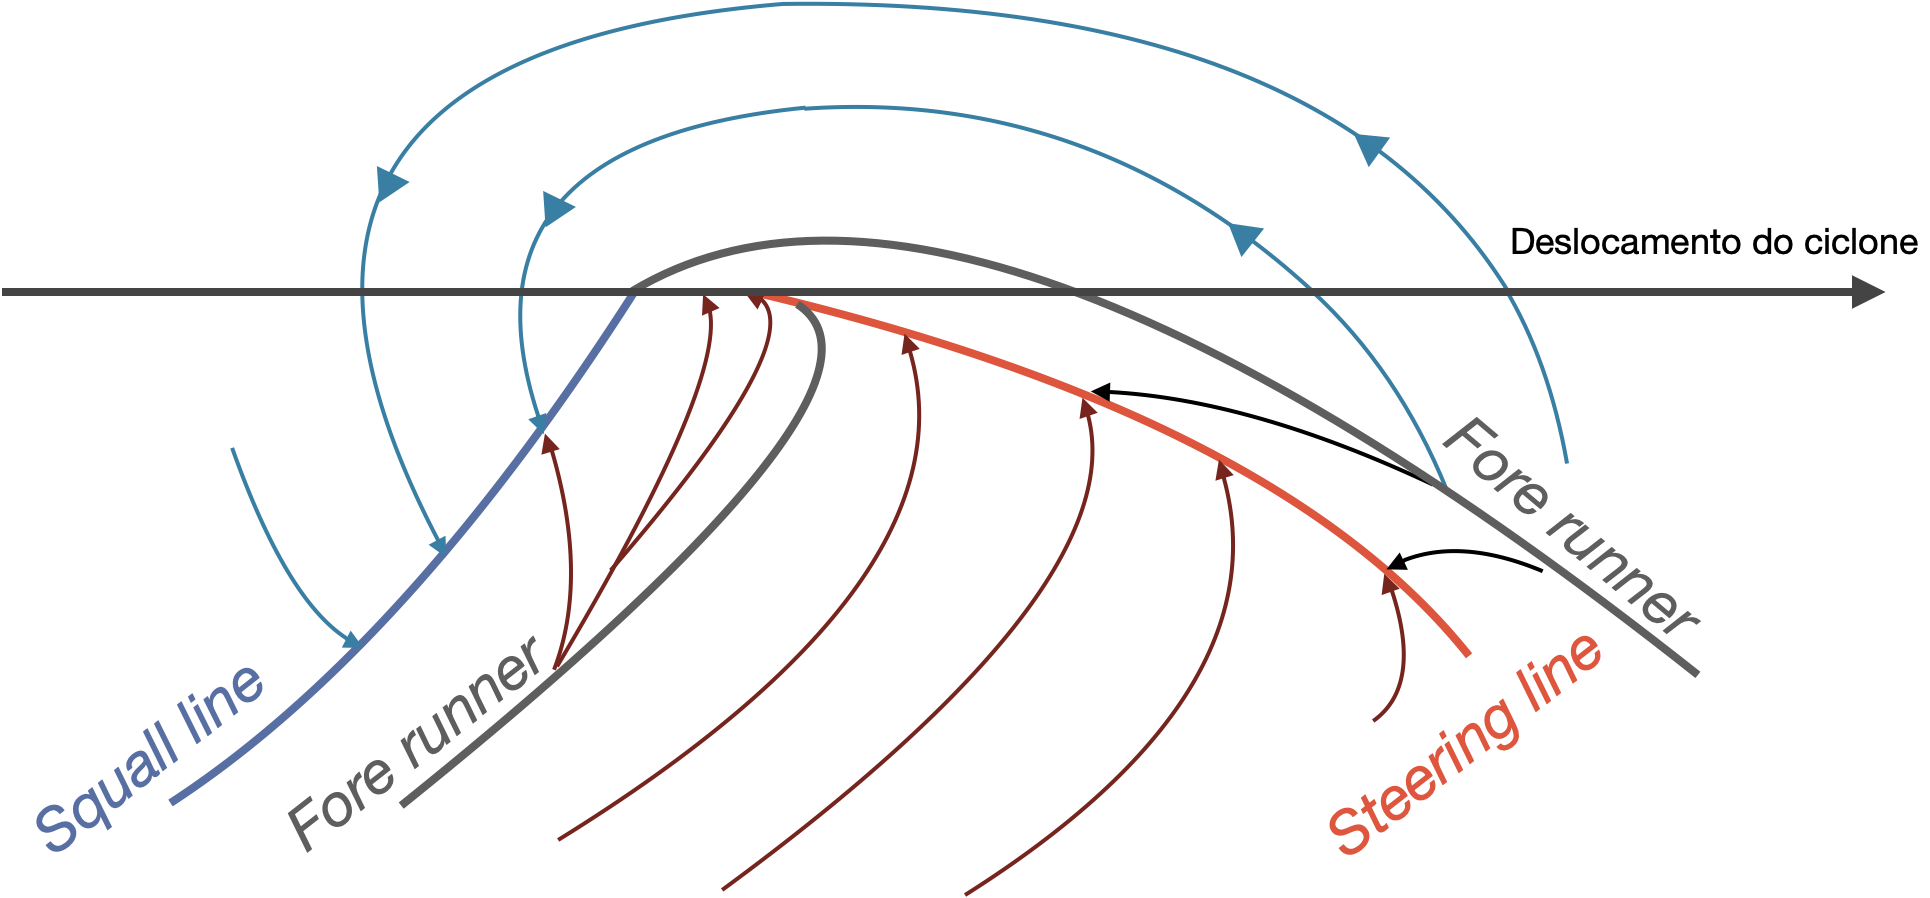
\includegraphics[width=0.7\columnwidth,angle=0]{fig/bjerknes_ciclone.png}
\caption[Bjerknes Cyclone Model]{Representation of the Bjerknes model for the extratropical cyclone formation process and its horizontal structure. Cold air regions are illustrated with blue lines, while warm air regions with red lines. Adapted from \citet{bjerknes1919structure}.} 
\label{bjerknes_cyclone}
\end{center}
\end{figure}

\citet{bjerknes1922life} realized that the model proposed in \citet{bjerknes1919structure} represented just one phase in the life cycle of cyclones, indicating that there are several stages of development. \citet{bjerknes1922life} established the Polar Front Theory, which is the foundation of the so-called Norwegian cyclone model. \citet{schultz1998effect} synthesizes and describes the development of extratropical cyclones according to this theory, so that a visual representation of the horizontal structure at the surface during different stages of cyclone evolution is found in Figure \ref{cyclone_models}a. In the first stage, the incipient cyclone presents a narrow and long cold front, and a wide and short warm front (Figure \ref{cyclone_models}aI). After this, the cyclone deepens, with a narrowing of the warm section of the cyclone through the rotation of the cold front towards the warm front (Figure \ref{cyclone_models}aII). As cold air is denser and, therefore, facilitates more intense horizontal pressure gradients, it moves faster than the warm air. As the cold air at the front of the cyclone approaches the cold air at the rear of the system (Figure \ref{cyclone_models}aIII), the warm air is trapped in the center of the system, a phenomenon called warm seclusion. As the cold front continues to move, the warm air at the surface is overtaken by the cold air and is forced to ascend to upper levels. This process is called occlusion, being responsible for trapping the cold air in the core of the system (Figure \ref{cyclone_models}aIV). With the continuation of occlusion, the baroclinicity along the warm front can become so diffuse that the cyclone appears not to have a well-defined warm front.

\citet{bjerknes1922life} acknowledged that the model presented in \citet{bjerknes1919structure} captured only a singular phase in the life cycle of cyclones, leading to the development of the Polar Front Theory. This theory defines what is known as the Norwegian cyclone model. \citet{schultz1998effect} provides a synthesis of extratropical cyclone development according to this theory, including a depiction of the surface horizontal structure at various stages of cyclone evolution in Figure \ref{cyclone_models}a. Initially, the nascent cyclone features a narrow, elongated cold front and a broader, shorter warm front (Figure \ref{cyclone_models}aI). Subsequently, the cyclone deepens as the cold front rotates toward the warm front, narrowing the cyclone's warm sector (Figure \ref{cyclone_models}aII). Given the greater density of cold air, which generates stronger horizontal pressure gradients and moves more swiftly than warm air, the cold front eventually encroaches on the system's rear cold air (Figure \ref{cyclone_models}aIII), trapping warm air at the system's center—a process known as warm seclusion. As the cold front progresses, the surface-level warm air is displaced by cold air and forced upward, a phenomenon termed occlusion, which entraps cold air at the system's core (Figure \ref{cyclone_models}aIV). The occlusion process may eventually diffuse the baroclinicity along the warm front to such an extent that the cyclone seems to lack a distinct warm front.

\begin{figure}[h]
\begin{center}
\setcaptionmargin{1cm}
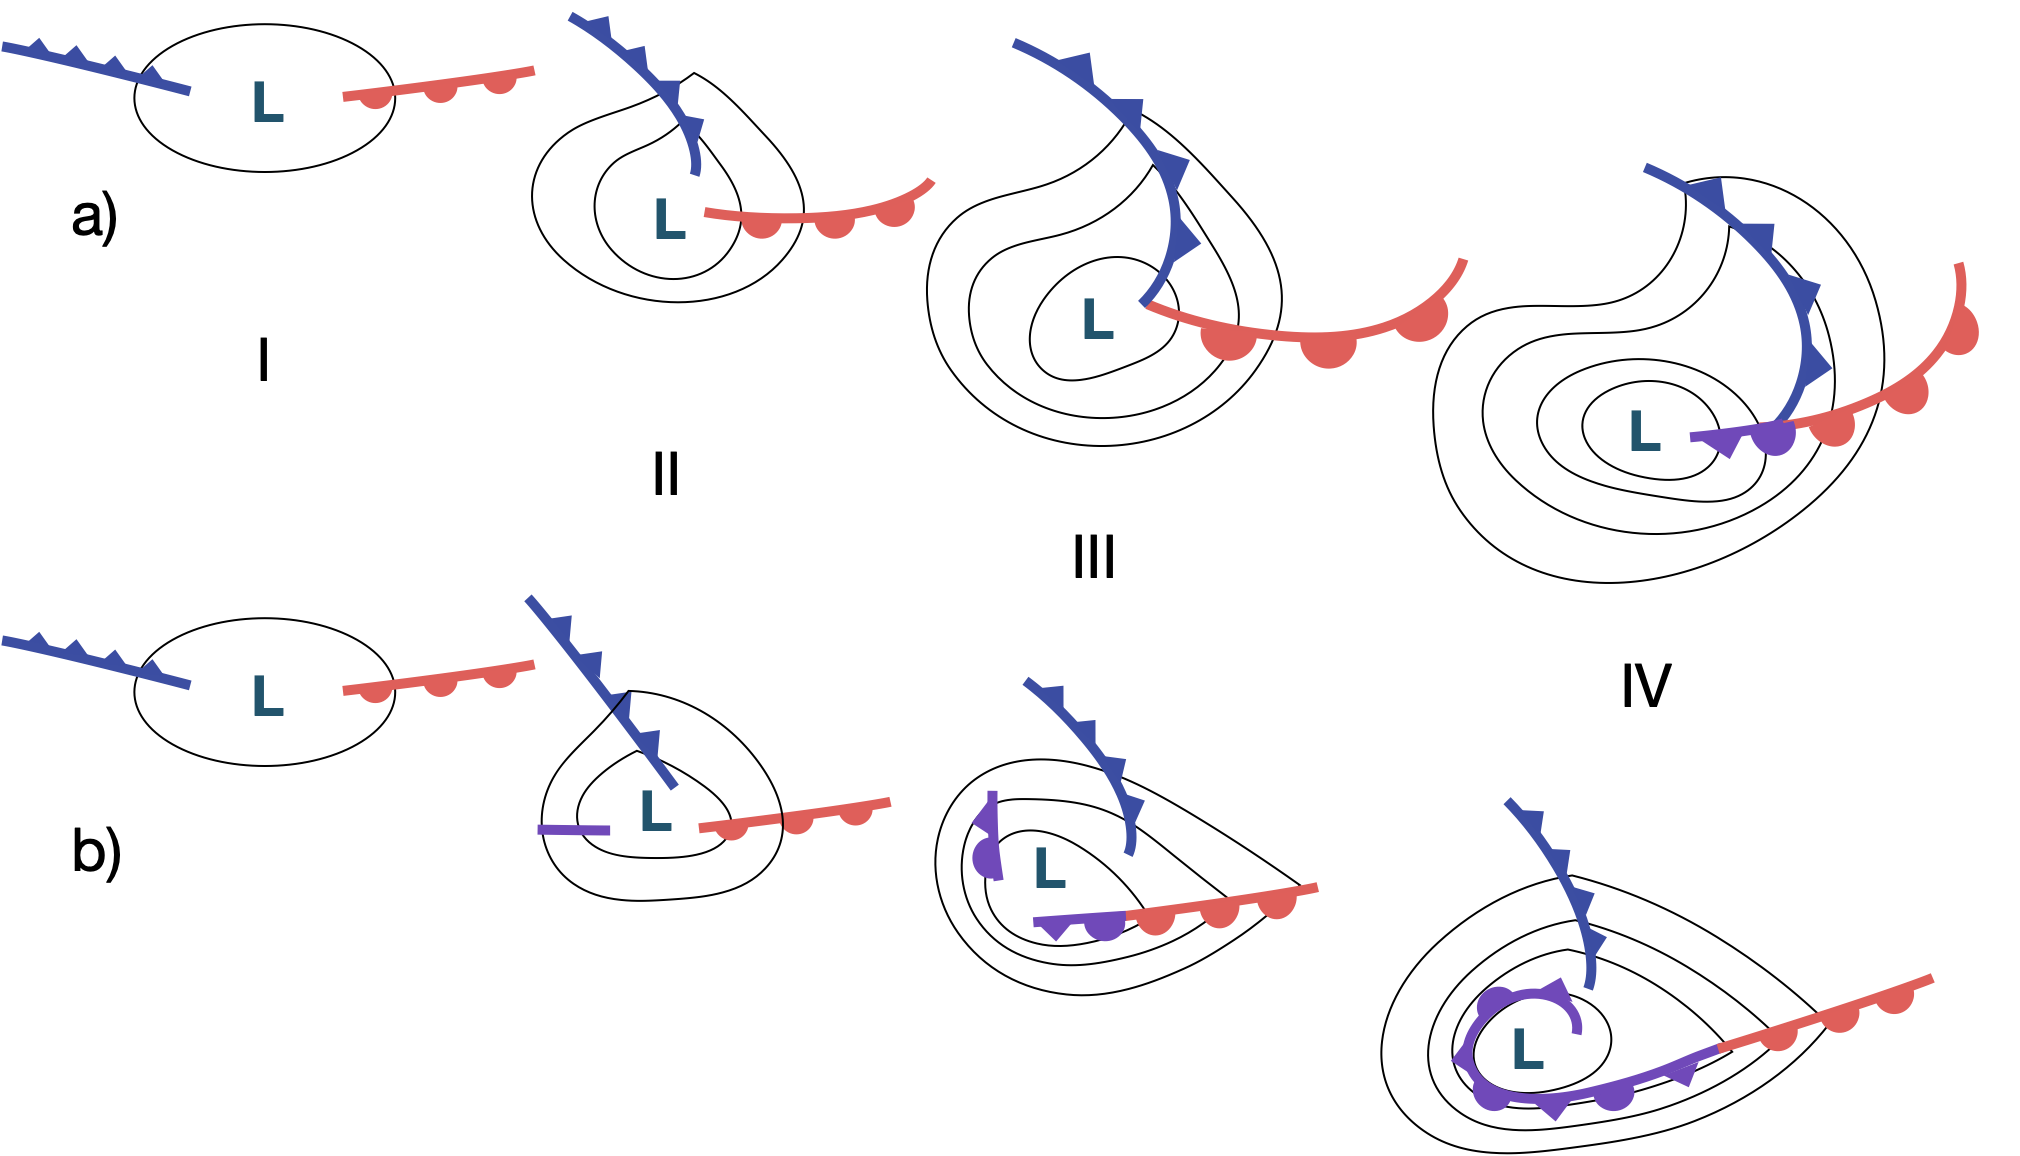
\includegraphics[width=0.7\columnwidth,angle=0]{fig/ciclones_modelos.png}
\caption[Bjerknes' and Shapiro-Keyser's Cyclonic Models]{Cyclonic models by \citet{bjerknes1919structure} (a) and \citet{shapiro1990fronts} (b), illustrating the systems' horizontal structure across different developmental stages (I to IV). Adapted from \citet{schultz1998effect}.}
\label{cyclone_models}
\end{center}
\end{figure}

From the advancements enabled by the satellite era, \citet{shapiro1990fronts} introduced a revised cyclonic model, acknowledging that not all observed cyclones conformed to the Norwegian model. Termed the Shapiro-Keyser model, it is also summarized by \citet{schultz1998effect}, with its visualization in (Figure \ref{cyclone_models}b). Initially mirroring the development outlined by \citet{bjerknes1922life} (Figure \ref{cyclone_models}bI), this model diverges as the cold front extends perpendicularly to the warm front instead of encircling the system (Figure \ref{cyclone_models}bII). As the system strengthens, the polar side of the cold front weakens, allowing the warm front to encircle the system's western sector (Figure \ref{cyclone_models}bIII). At peak intensity, cold air encases the warm air near the cyclone's center, creating a warm seclusion (Figure \ref{cyclone_models}bIV).

\citet{schultz1998effect} emphasizes that these models are complementary rather than mutually exclusive, suggesting that the Norwegian model is more applicable to systems forming under diffluent flow with significant amplitude, often at the terminal end of storm tracks and on western continental edges, characterized by a meridional elongation of the cyclone and its fronts. Conversely, the Shapiro-Keyser model is more suited to systems emerging under confluent, low amplitude base flow, typically exhibiting east-west elongation. However, these models alone do not fully account for the formal causes of extratropical cyclones, indicating a continuum where different systems may align more closely with one model or the other \citep{schultz1998effect}.

Tropical cyclones, unlike their extratropical counterparts, lack frontal structures and exhibit organized, symmetric circulation near the surface, forming over warm tropical or subtropical waters with intense winds below the surface \citep{frank1977structurea, gray1968global}. Their diameters vary, ranging from 100 to 1000 km at maturity, expanding up to 2000 km during intensification. However, the area of intense convection and stronger winds typically spans a radius of about 100 km \citep{holton1973introduction}.

Characterized by a central cyclonic circulation at lower tropospheric levels and anticyclonic circulation in the upper troposphere, tropical cyclones are associated with intense precipitation and horizontal pressure gradients, leading to spiraled winds near the surface that become increasingly circular towards the system's center, or eye \citep{frank1977structurea,frank1977structureb,terry2007tropical, weatherford1988atyphoon}. These systems exhibit more intense pressure gradients—and consequently stronger winds—than extratropical cyclones \citep{spiridonov2021fundamentals}. Based on wind speed, they are classified into tropical depressions (maximum winds less than 60 km/h), tropical storms (winds between 60 and 110 km/h), and tropical cyclones (winds exceeding 110 km/h) \citep{spiridonov2021fundamentals}. Their nomenclature varies by region: "hurricanes" in the North Atlantic and North Pacific, "typhoons" in the Northwest Pacific, and "cyclones" in the Indian Ocean \citep{donald2015meteorology}.

The structure of tropical cyclones comprises three main components: the eye, the eye wall, and surrounding convection bands (Figure \ref{hurricane_cross_section}). The eye is the calm, warm central region, with a radius of 5 to 50 km, encircled by the eye wall—a cloud ring about 10 to 20 km wide where intense upward vertical movements occur, facilitating mass transport to higher levels \citep{shea1973hurricane,jorgensen1985vertical}. Although these vertical movements are typically less vigorous than those in extratropical cyclones \citep{jorgensen1985vertical}, the inner core, consisting of the eye and eye wall, hosts the most intense winds and lowest atmospheric pressures \citep{weatherford1988atyphoon}. The primary convection band, a nearly stationary feature, spirals inward from the system's outer edges towards the eye wall, where it becomes roughly tangent \citep{willoughby1984stationary}.

\begin{figure}[h]
\begin{center}
\setcaptionmargin{1cm}
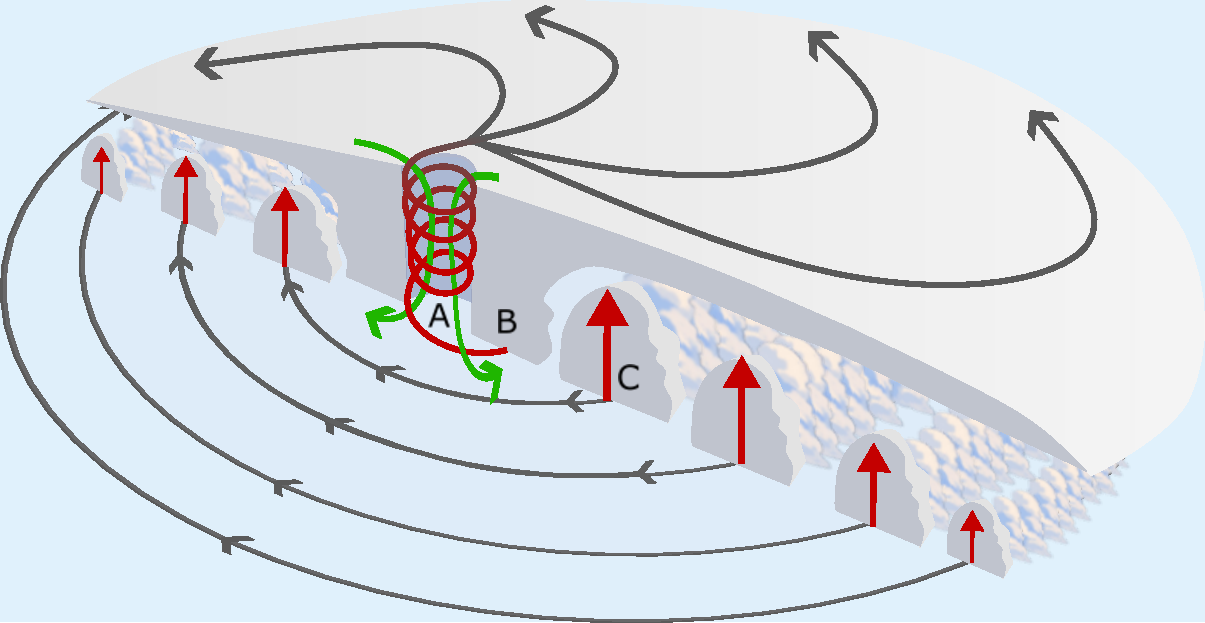
\includegraphics[width=0.7\columnwidth,angle=0]{fig/hurricane_cross_section.pdf}
\caption[Tropical Cyclone - Cross Section]{Cross-sectional view of a mature tropical cyclone in the Southern Hemisphere, illustrating the eye (A), eye walls (B), and convection bands (C), along with upward (red arrows) and downward (green arrows) vertical movements, horizontal wind movement (grey arrows), and sea-level pressure contours. Inspired from: \citet{bluestein1992synoptic}.} 
\label{hurricane_cross_section}
\end{center}
\end{figure}


Given the delineated formal causes (organizational structure) for both extratropical and tropical cyclones, it's evident that their structures diverge significantly. Simplified, extratropical cyclones, forming at the interface between distinct air masses, are associated with frontal systems, providing them an asymmetric feature. Conversely, tropical cyclones exhibit symmetry, characterized by a circular eye and spiraled convection bands extending from the eye wall. Addressing this distinction, \citet{hart2003cyclone} introduces a metric assessing the relative thickness asymmetry between the 900 and 600 hPa levels, termed the \(B\) parameter:


\begin{equation}
    B = h \left(\overline{Z_{600 hPa} - Z_{900 hPa}}|_R - \overline{Z_{600 hPa} - Z_{900 hPa}}|_L \right)
\end{equation}

where \(Z\) represents the isobaric height, \(R\) and \(L\) denote the right and left sides relative to the system's motion, the overbar signifies an average over a 500 km semicircle, as defined in Equation \ref{height_pertubation}, and \(h\) is a constant set to +1 or -1 for the northern and southern hemispheres, respectively. Mature tropical cyclones exhibit a \(B\) value near zero, indicating thermal symmetry (non-frontal), while extratropical cyclones show significant \(B\) values, signaling thermal asymmetry (frontal). Positive \(B\) values suggest the presence of warm air to the right of the cyclone in the southern hemisphere (and vice versa in the northern hemisphere), aligning with the thermal wind relationship from quasi-geostrophic theory \citep{sutcliffe1947contribution, trenberth1978interpretation}.

\citet{hart2003cyclone} proposed a diagram correlating symmetry with \(V^{L}_{T}\) (Equation \ref{eq_VTL}), depicted in Figure \ref{phase_space_Hart_2}, offering a supplementary classification to that shown in Figure \ref{phase_space_Hart_1}. Here, extratropical cyclones are categorized as cold and asymmetric (frontal), whereas tropical cyclones are warm and symmetric (non-frontal). Like the earlier diagram, this classification suggests a continuum, with systems displaying intermediate features labeled as subtropical. Unlike solely thermal-based classifications, this model allows for differentiation of extratropical cyclones undergoing occlusion, as these systems begin to exhibit symmetry during this phase. Hence, the diagram involving the \(B\) parameter and \(V^{L}_{T}\) presents an objective methodology to classify cyclones' formal causes.

While the phase diagrams by \citet{hart2003cyclone} facilitate objective classification criteria for cyclonic systems, gaps remain. For instance, warm seclusions share formal and material causes with hybrid systems, leading to potential misclassification by forecasters and climate data analysis algorithms using these diagrams exclusively. Additionally, polar lows, characterized by both a warm core and symmetric structure, were initially likened to hurricanes \citep{rasmussen1989comparative,emanuel1989polar,nordeng1992most,rasmussen1985case,rasmussen1979polar}. However, recent studies, such as \citet{stoll2021polar}, suggest their spiral bands and thermal core may result from the warm seclusion process, as per the Shapiro-Keyser cyclone development model. These discussions underscore that material and formal causes alone do not suffice for a comprehensive cyclone classification, necessitating further analysis.

\begin{figure}[h]
\begin{center}
\setcaptionmargin{1cm}
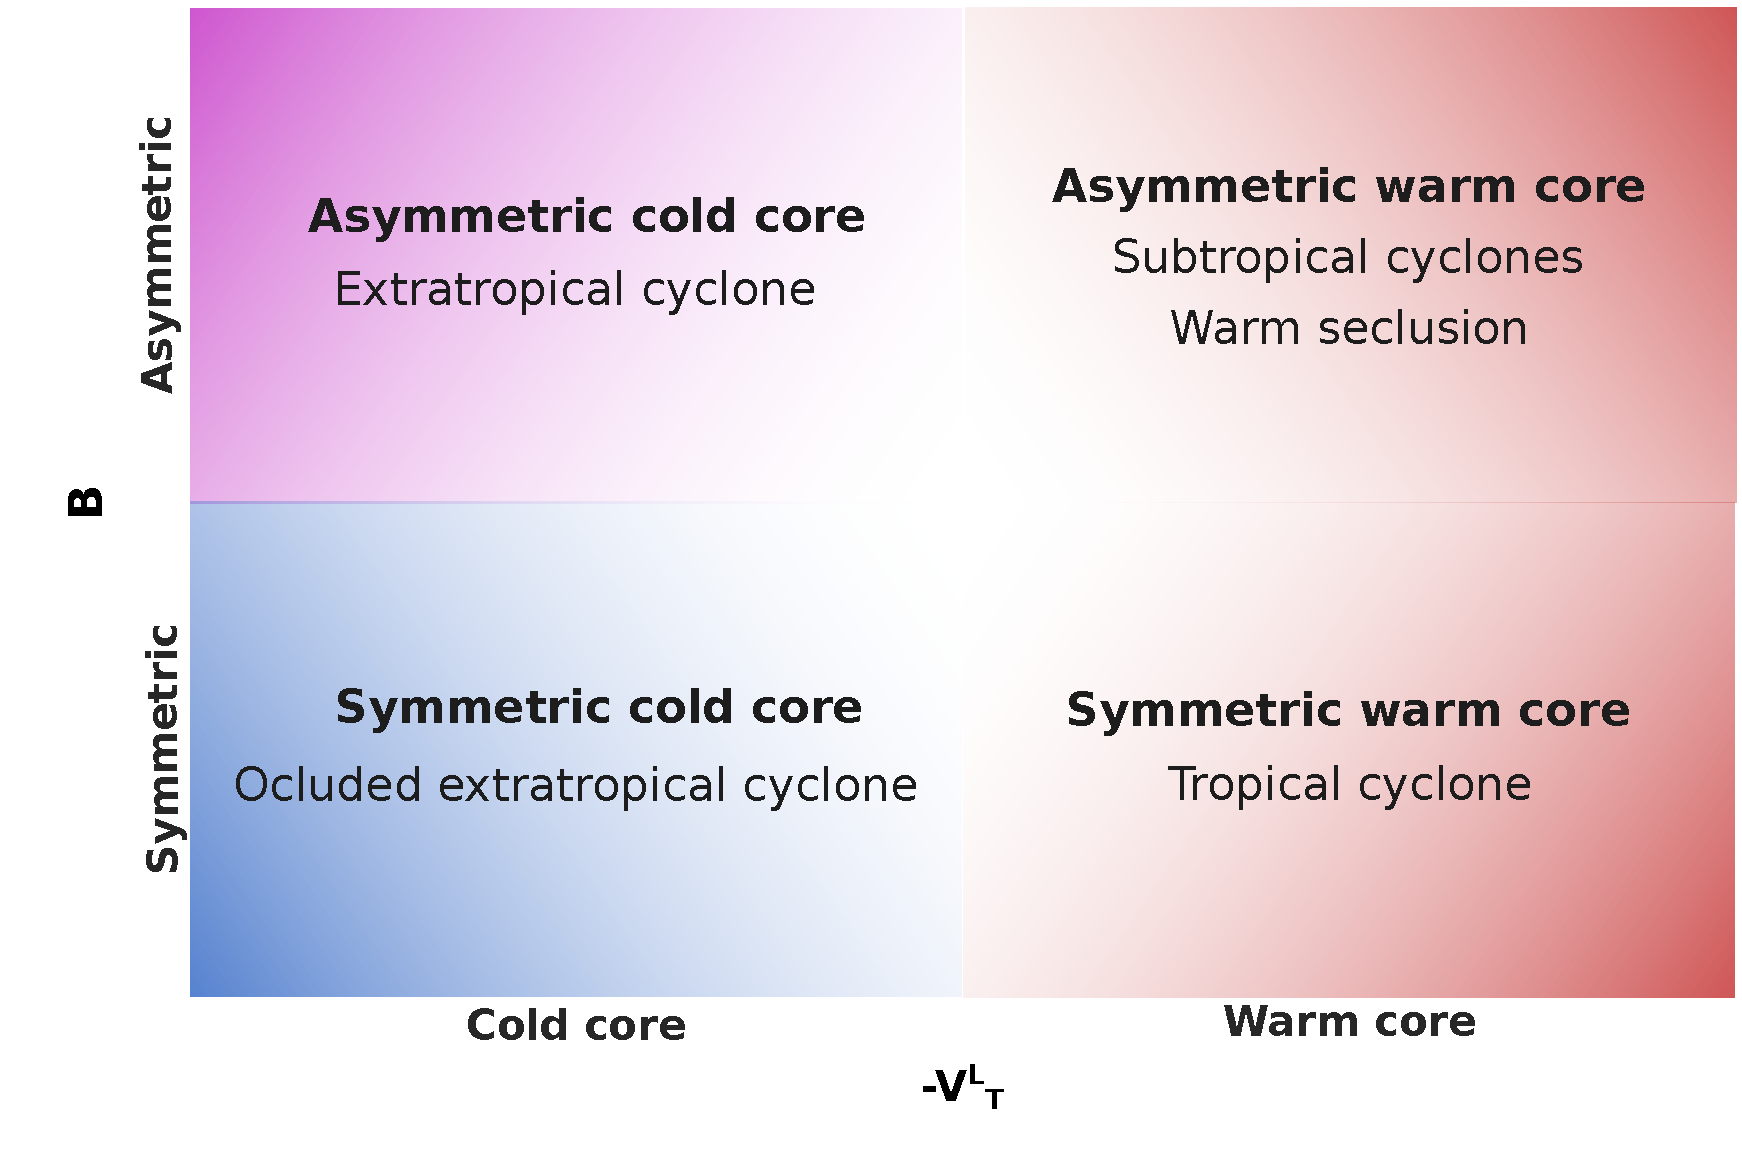
\includegraphics[width=0.7\columnwidth,angle=0]{fig/hart_diagram_2.pdf}
\caption[Phase Diagram - Hart]{Phase diagram illustrating the relationship between cyclonic systems' core temperature and symmetry, offering a distinct classification procedure. Adapted from \citet{hart2003cyclone}.}
\label{phase_space_Hart_2}
\end{center}
\end{figure}


\subsection{Efficient Causes}\label{efficient_causes}

The efficient cause represents the agent or process that leads to the creation or transformation of something, answering the "how" or "why" behind an occurrence. It encompasses the actions or processes that result in the existence of an entity. For example, in the creation of a table, the carpenter serves as the efficient cause. In the context of cyclones, the efficient cause includes the physical and dynamic processes responsible for their formation and intensification. These processes essentially act as destabilization mechanisms, triggering atmospheric disturbances that evolve into a cyclonic configuration.

While the polar front theory offers a descriptive perspective, it falls short of providing a comprehensive theoretical model for the physical processes involved in system formation. Still, it related these processes with thermal contrasts in the atmosphere, or baroclinic zones \citep{bjerknes1919structure,bjerknes1922life}, describing cyclones as emergent phenomena arising at the boundary of two distinct air currents—polar and tropical—flowing in opposite directions (east-west and west-east, respectively), differentiated by thermal contrasts (cold and warm, respectively). A destabilization of the flow occurs when the velocity difference between these currents surpasses a critical threshold, generating a frontal wave that intertwines the currents and reduces their velocity contrast. Some of these frontal waves are unstable and can spontaneously amplify, representing the genesis mechanism of cyclones according to this theory.

The Polar Front Theory provides a detailed account of the structure and formation processes of extratropical cyclones, as shown in Figure \ref{extratropical_cyclone_transversal}, depicting a transverse model of a developing cyclone \citep{bjerknes1922life}. This model features horizontal isotherms indicative of temperature variations parallel to the ground, with warm air central to the model, characteristic of the warm front, and cold air on the edges. Initially (Figure \ref{extratropical_cyclone_transversal}a), the isotherms of cold air extend horizontally until convergence forces the ascent of warm air to higher atmospheric levels. This conversion of potential to kinetic energy continues as the cold air from both sides of the cyclone advances to mid-atmospheric levels, further driving the ascent of warm air. The adiabatic cooling of ascending warm air leads to temperature equalization and depletion of the system's potential energy reserve, while the air mass movement is then sustained by inertia. After occlusion (Figure \ref{extratropical_cyclone_transversal}b and c), inertia maintains the ascent of cold air, which cools adiabatically, utilizing the system's kinetic energy to counteract gravity. Initially, there is still kinetic energy production at high levels and its consumption at low levels. However, as the elevated warm sector cools and temperatures equalize (Figure \ref{extratropical_cyclone_transversal}d), kinetic energy production halts. Eventually, friction outweighs kinetic energy production, leading to its dissipation.

\begin{figure}[h]
\begin{center}
\setcaptionmargin{1cm}
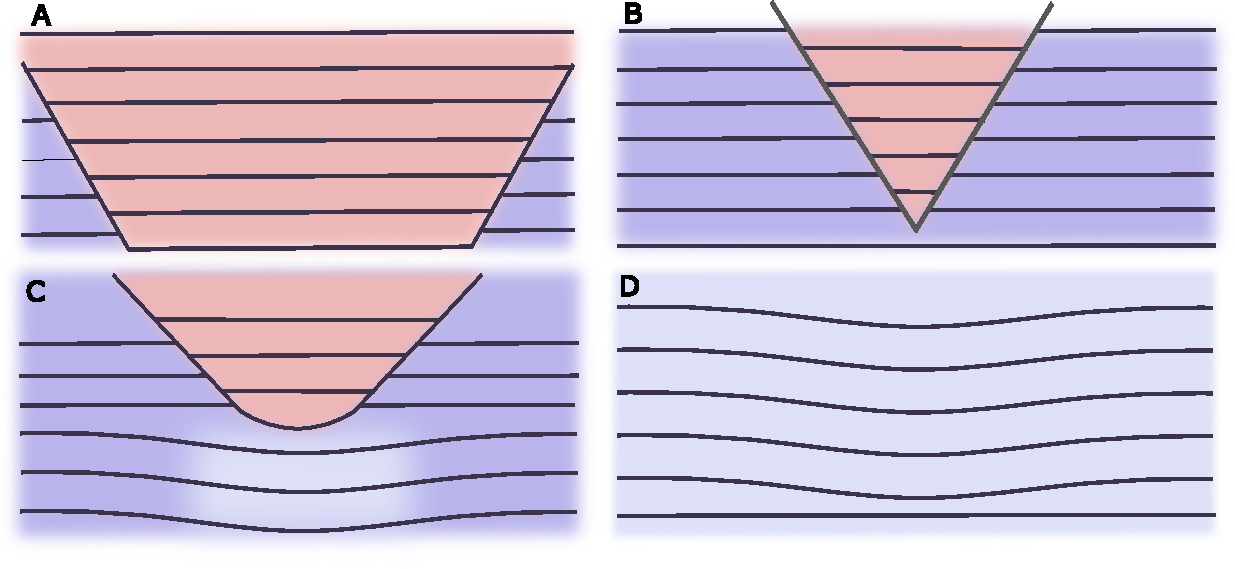
\includegraphics[width=0.7\columnwidth,angle=0]{fig/ciclone_oclusion.pdf}
\caption[Extratropical Cyclone - Cross Section]{Cross-sectional depiction of an extratropical cyclone's development through its various stages, adapted from \citet{bjerknes1922life}. Stage A shows horizontal isotherms where cold air converges, leading to the ascent of warm air. In Stage B, the system begins occlusion as cold air advances to mid-atmospheric levels, further promoting the ascent of warm air. Stage C continues the occlusion, with sustained ascent of cold air by inertia and kinetic energy consumption. Stage D represents the cessation of kinetic energy production as temperatures equalize and friction begins to dominate, leading to energy dissipation. Warm (red) and cold (blue) sectors are indicated alongside the isotherm lines.}
\label{extratropical_cyclone_transversal}
\end{center}
\end{figure}

Since the advent of the polar front theory, our comprehension of atmospheric dynamics has evolved significantly, incorporating new concepts into the understanding of extratropical cyclones. This evolution has led to a diverse array of approaches aimed at describing the dynamic and thermodynamic processes underlying the genesis and development of these systems. Consequently, there is no singular, unified theory regarding extratropical cyclogenesis. For instance, \citet{bjerknes1944theory} identified the formation regions of extratropical cyclones as zones of dynamic instability associated with the westward-flowing jet stream, employing the tendency equation to analyze atmospheric instability. Other studies have approached cyclogenesis through various lenses, including slantwise convection, the omega equation, potential vorticity, primitive equations, and diabatic processes \citep[e.g.]{hoskins1990theory}. Additionally, \citet{schultz1998effect}'s work categorizes cyclones into those aligning with the Norwegian model versus the Shapiro-Keyser model, differentiating them based on environmental conditions related to the base state flow (diffluent for the former and confluent for the latter). This section will primarily focus on the development of these systems from the perspective of dynamic destabilization mechanisms in the atmosphere, linking these mechanisms to the energetics of transient atmospheric systems, further explored in Section \ref{atmosphere_energetics}.


Baroclinic instability (\(I_{BC}\)) is identified as the principal mechanism behind the development of typical extratropical cyclones \citep{charney1947dynamics, bjerknes1922life}. As \citet{holton1973introduction} explains, \(I_{BC}\) involves the amplification of small disturbances in areas with strong velocity shears, such as jet streams, where the disturbances extract energy from the jet and grow in size and intensity. In the Earth's atmosphere, \(I_{BC}\) is primarily driven by the meridional temperature gradient, especially at lower levels, and is linked to vertical shear via the thermal wind (\(V_T\)) relationship, frequently occurring in the polar frontal zone. Baroclinic disturbances can also intensify existing temperature gradients, leading to the formation of frontal zones.

\citet{charney1947dynamics}'s seminal study on \(I_{BC}\) sheds light on the intricate mechanisms behind the formation and evolution of weather patterns, including cyclones and long waves in middle and high latitudes. Employing a simplified model that allows for analytical solutions, Charney not only corroborated previously theorized concepts about atmospheric behavior but also deepened the understanding of how wind shear and temperature variations vertically contribute to atmospheric instability. His analysis indicates that mid-latitude westward-flowing currents are inherently dynamically unstable. This insight elucidates how specific disturbances can exponentially grow within a large-scale atmospheric flow field, explicating the process through which such disturbances can amplify and culminate in the characteristic weather systems observed in middle and high latitudes.

\citet{eady1949long} made significant advancements in the understanding of \(I_{BC}\) in the atmosphere, building on the work of \citet{charney1947dynamics}. Eady's research, which employed a solvable simplified model, delved into the atmospheric instability arising from disturbances that exponentially grow within a large-scale atmospheric motion context. His analysis elucidated how specific conditions of stability, wind shear, and vertical temperature variations contribute to \(I_{BC}\), proposing a mechanism for the formation and evolution of weather patterns such as cyclones and long waves in middle and high latitudes. Eady highlighted that certain disturbances grow exponentially faster than others, akin to a process of natural selection in the atmosphere, leading to the emergence of predominant weather patterns observed in middle latitudes, including cyclonic systems.

Following the seminal works of \citet{charney1947dynamics} and \citet{eady1949long}, \citet{palmen1969atmospheric} synthesized the main findings from the subsequent extensive literature on \(I_{BC}\). Firstly, it is noted that the amplification of atmospheric disturbances is wavelength-dependent, with disturbances below a critical length never amplifying. The optimal growth occurs in intermediate wavelengths (between 2500 and 5000 km), with an inverse relationship between this optimum and latitude—the closer to the Equator, the larger the critical size below which all waves are unstable. Additionally, there exists a proportional relationship between the intensification rate and vertical wind shear for wavelengths of maximum instability, and for longer waves, an increase in wavelength necessitates stronger shear to maintain equivalent growth rates.

In his analysis, \citet{petterssen1971development} categorizes extratropical cyclones into types based on the dynamic processes driving their development. Type A cyclones follow the Polar Front Theory model, with the initial disturbance arising at low levels within a maximal baroclinic zone (frontal), beneath a nearly zonal upper-level jet (Figure \ref{cyclone_pettersen}iA). As these cyclones develop, a cold trough forms at high levels (Figure \ref{cyclone_pettersen}iB), remaining inclined to the cyclone's axis until occlusion occurs and surface baroclinicity diminishes (Figure \ref{cyclone_pettersen}iC). Conversely, type B cyclones initiate from high-level forcing, as an upper-level trough moves over an area not necessarily featuring a frontal zone (Figure \ref{cyclone_pettersen}iiA). As these systems mature, the gap between the high-level trough and the surface system narrows, with an increase in surface baroclinicity relative to the initial stage (Figure \ref{cyclone_pettersen}iiB), culminating in the alignment of the high-level cyclonic vortex with the surface low, leading to system occlusion (Figure \ref{cyclone_pettersen}iiC).

\begin{figure}[h]
\begin{center}
\setcaptionmargin{1cm}
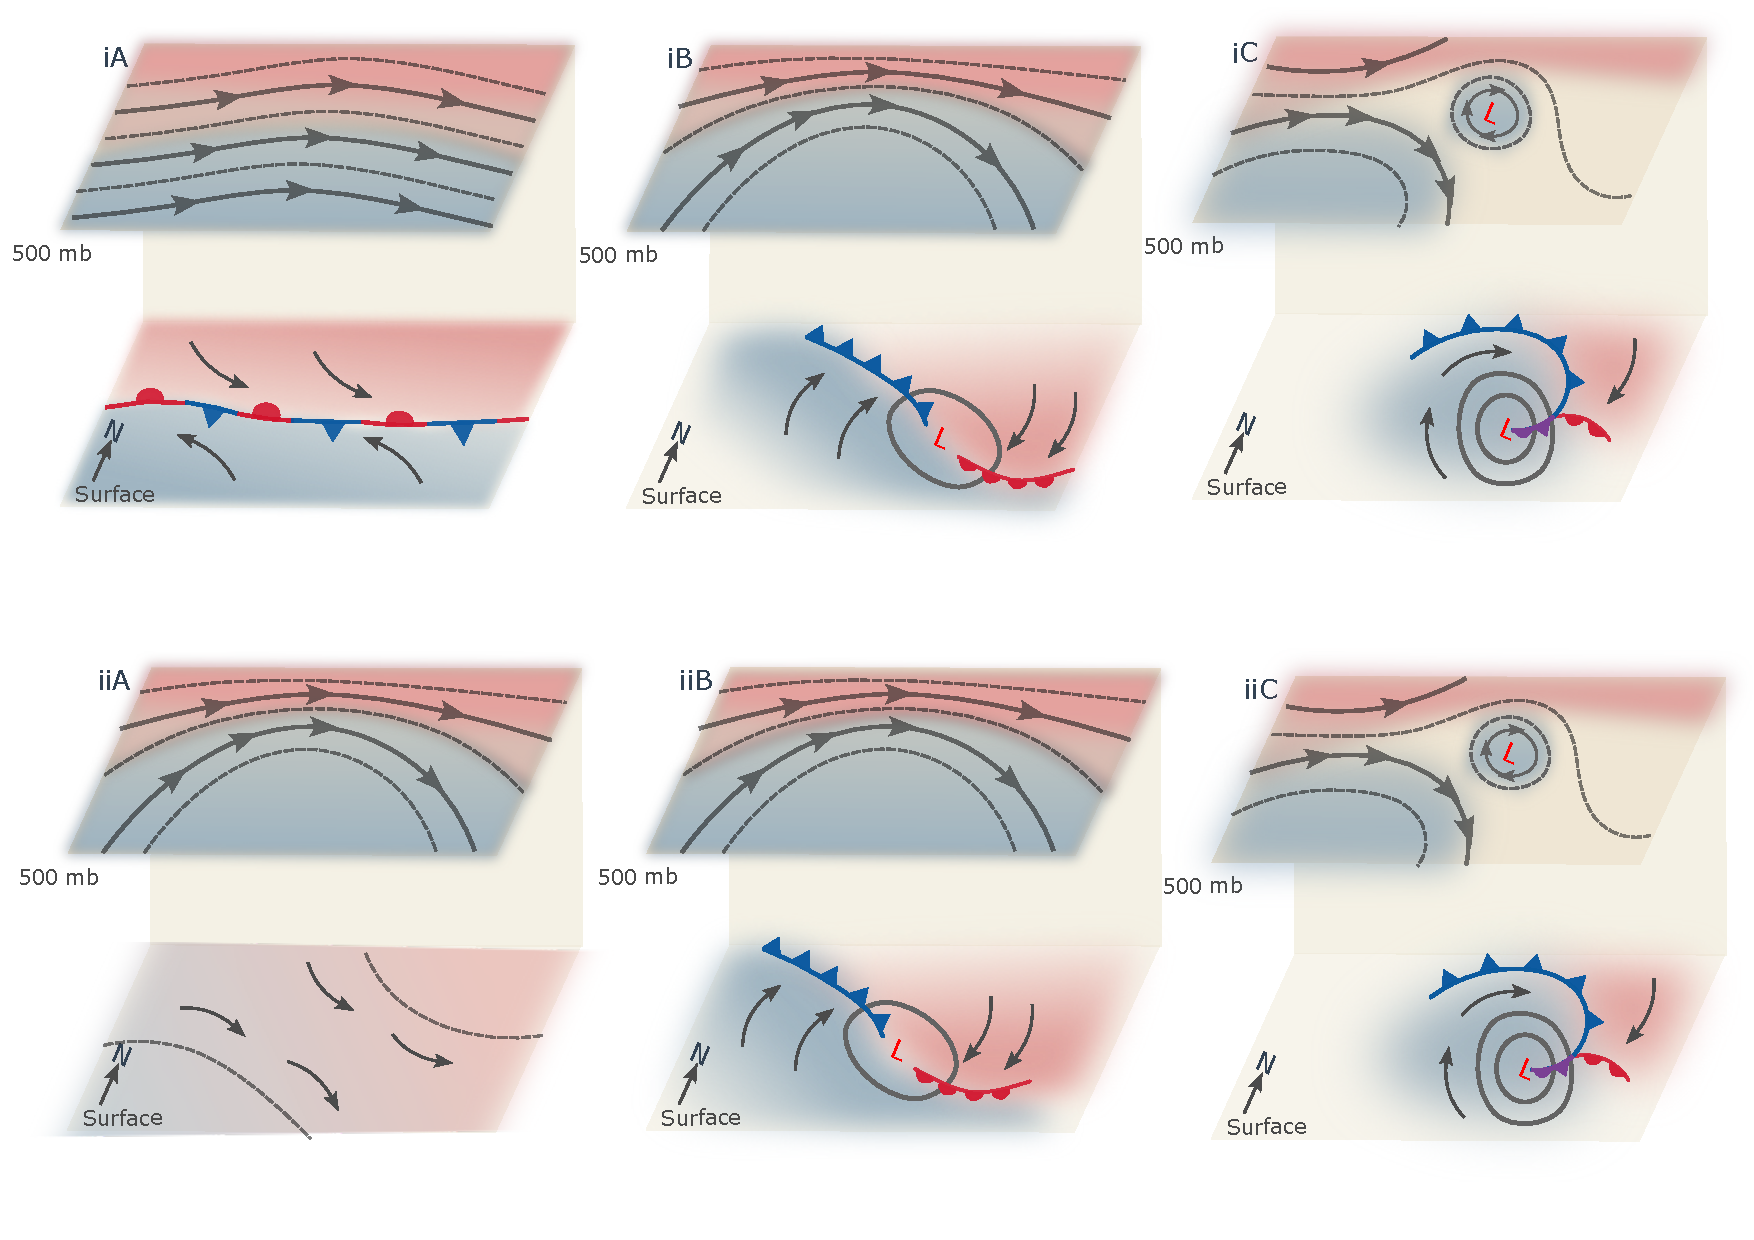
\includegraphics[width=1\columnwidth,angle=0]{fig/cyclone_pettersen.pdf}
\caption[Model of development of cyclones types A and B.]{Illustration of the development model for cyclones types A (i) and B (ii), depicting the stages of formation (A), intensification (B), and maturity (C), as proposed by \citet{petterssen1971development}. Inspired by \citet{donald2015meteorology}.}
\label{cyclone_pettersen}
\end{center}
\end{figure}

Just as \citet{hart2003cyclone}'s classification presents a continuum, so too does \citet{petterssen1971development}'s delineation of cyclone types, with A and B not being distinct categories due to the existence of systems displaying hybrid characteristics. \citet{petterssen1971development} observed that purely type A cyclones are more common, whereas purely type B cyclones are rare, attributing this to the fact that some type of baroclinicity is often present in the mid-latitudes. However, Petterssen noted a tendency for type A cyclones to develop over oceans and type B cyclones over continents, though subsequent research, such as by \citet{mclennan1988marine} and \citet{deveson2002classification}, has identified type B systems forming over oceanic regions as well. Furthermore, \citet{deveson2002classification} introduced a new classification, type C cyclones, found in high latitudes with similarities to polar lows, characterized by an even stronger high-level forcing related to the movement of a broad trough over oceanic regions. This study also highlighted the potential for cyclones to transition between types throughout their lifecycle.

The central role of baroclinic instability (\(I_{BC}\)) in the development of extratropical cyclones is well-established, yet the significance of heat flows and diabatic heating cannot be overstated. Diabatic heating involves heat exchanges between a system and its surroundings through processes such as condensation, evaporation, or radiation. Convective activities leading to upward atmospheric movements cause diabatic expansion and thus cooling in air parcels, leading to saturation and the release of latent heat. Such mechanisms provide an additional energy source for the development of extratropical cyclones, as documented in the literature \citep[e.g.]{chang2002storm}. Numerical models incorporating \(I_{BC}\) alongside heat flows have shown that instabilities generated under these conditions yield more intense cyclones with faster development rates \citep{gall1976effects,whitaker1994cyclogenesis,gutowski1992life}, a phenomenon referred to as moist baroclinic instability.

A pivotal study by \citet{hoskins1990existence} underscores the importance of diabatic fluxes in the development of extratropical cyclones, demonstrating that cyclonic development is preferentially located in regions of maximal baroclinicity over the oceans. However, the heat transport facilitated by these systems tends to mitigate the baroclinicity. The study suggests that diabatic heating, through the latent heat release from individual systems, contributes to sustaining regional baroclinicity. It also highlights the role of sensible heat exchanges between the cold air associated with these systems and the warm ocean currents along the eastern coastlines of continents.

Tropical cyclone formation, a topic of ongoing discussion among meteorologists, typically occurs over tropical or subtropical oceans, a region where the scarcity of in situ observations challenges the validation of theoretical models for formation and intensification. During World War II, data collected from the military base in Guam facilitated \citet{riehl1948formation} in proposing that the instability necessary for typhoon formation originates within the trade winds, contradicting the then-prevailing belief of inter-hemispheric air mass interactions being the primary cause. Subsequently, \citet{yanai1961detailed}'s study on Typhoon Doris furthered the understanding of typhoon genesis, highlighting the significant role of latent heat released by convection. Yanai suggested a model for typhoon development, beginning with a disturbance in the trade winds and culminating in the formation of a typhoon characterized by a stabilized warm core.

\citet{charney1964growth} detailed the process of tropical cyclone intensification known as conditional instability of the second kind (CISK), which was the most accepted theory at the time (Figure \ref{cisk_wishe}i). According to CISK, the condensation of water vapor within convective areas releases latent heat, which can amplify pre-existing atmospheric vortices given an adequate moisture supply. This release of heat not only promotes further convection but also lowers sea-level pressure, thereby strengthening surface winds, enhancing moisture influx, and establishing a positive feedback loop. Charney underscored the ocean's surface role in providing the moisture necessary for sustaining convection, as well as the importance of surface friction in dissipating kinetic energy and fostering wind convergence within the moist surface boundary layer, thereby fueling the system with thermal energy from latent heat. This mechanism emphasizes the pivotal role of latent heat release at the cyclone's center as a disturbance amplification factor, leading to the intensification of the tropical depression.

\begin{figure}[h!]
\begin{center}
\setcaptionmargin{1cm}
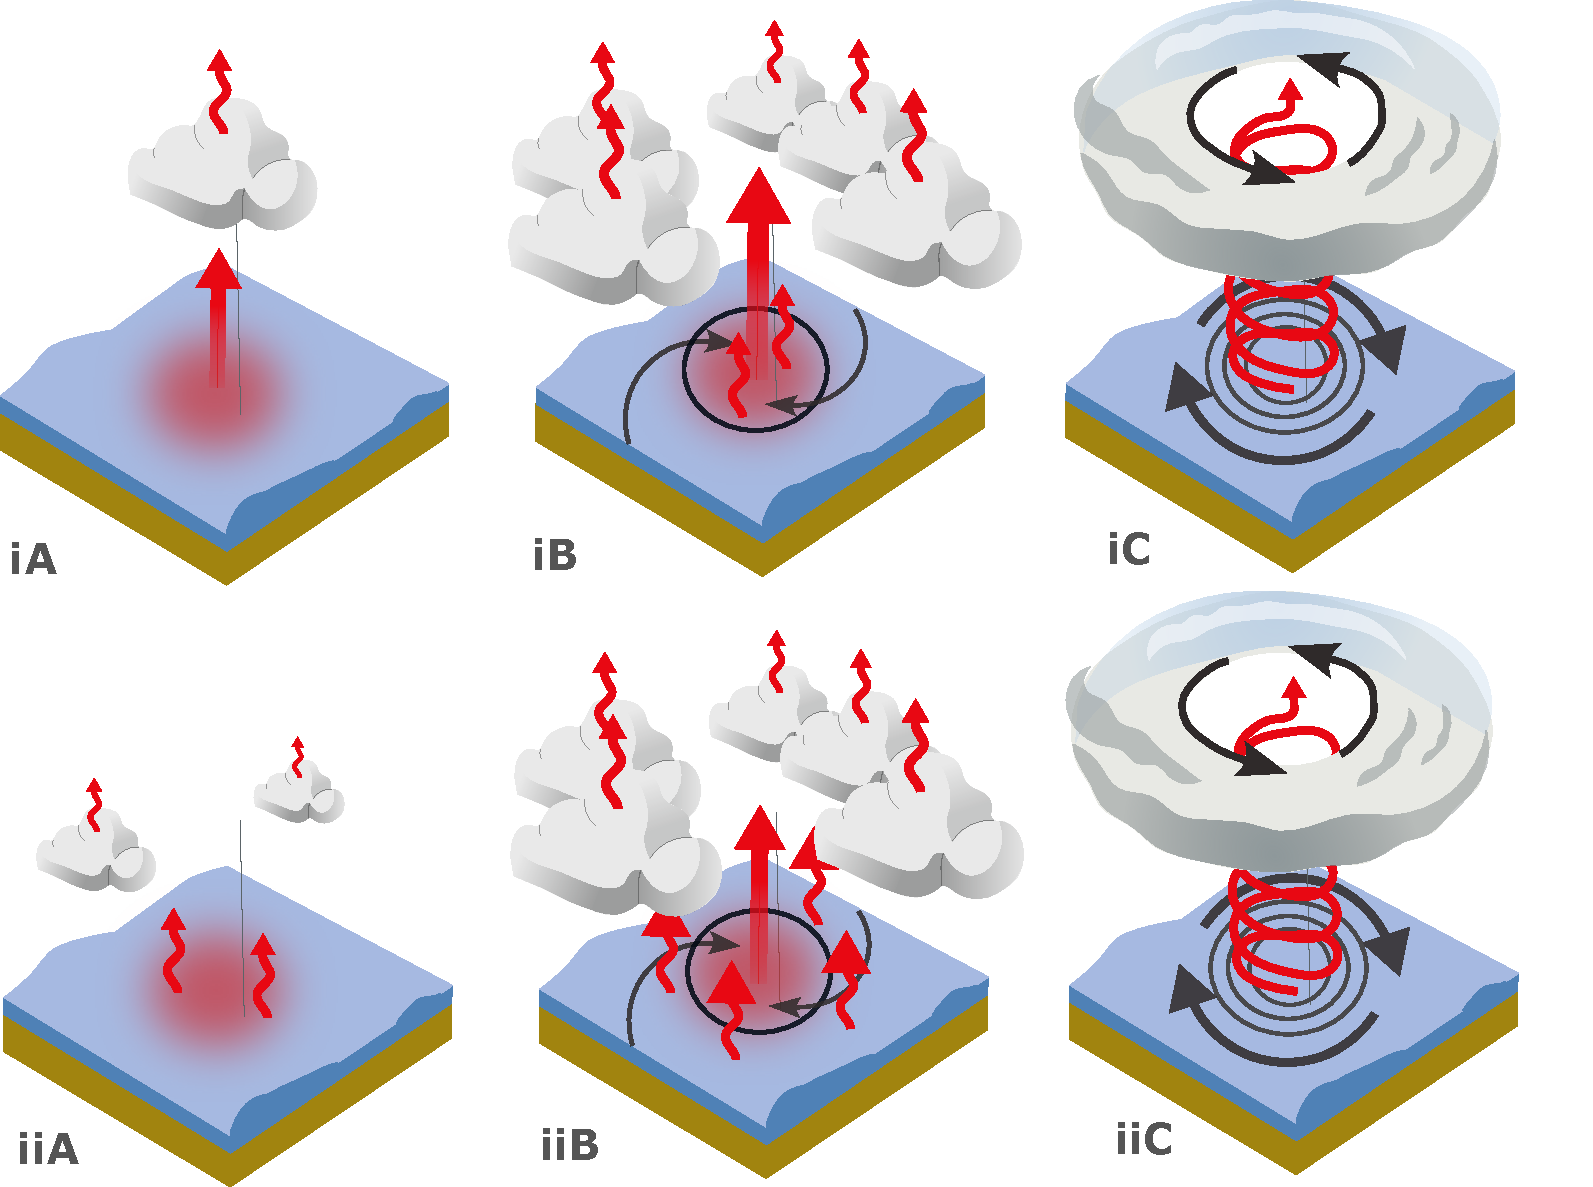
\includegraphics[width=0.9\columnwidth,angle=0]{fig/CISK_WISHE.pdf}
\caption[Comparison - CISK vs. WISHE]{Comparative illustration of the CISK (i) and WISHE (ii) theories. A depicts the initial disturbance over warm ocean temperatures. Under CISK, the disturbance is initially fueled by latent heat from convection, whereas WISHE attributes the initial energy source to latent heat transfer from the ocean to the atmosphere. In the early development stage (B), both theories observe an increase in convection. CISK suggests this leads to reduced central pressure, drawing in more moisture and enhancing convection, which releases additional heat. WISHE proposes that surface wind interaction with the sea surface at low central pressure enhances heat release from surface water evaporation, further driving convection and subsequent latent heat release. By the tropical storm phase (C), the theories align on the feedback mechanisms fueling system intensification.}
\label{cisk_wishe}
\end{center}
\end{figure}

However, it is important to note that the work of \citet{charney1964growth} consists of formulating a mathematical model and, therefore, does not offer a direct and didactic explanation of the processes involved. Thus, the interpretation of the proposed mechanisms is largely left as an exercise for the reader, which has resulted, over the years, in multiple interpretations, not all of them correct \citep{ooyama1982conceptual}. Therefore, the explanation provided above seeks only to simplify the main processes proposed by \citet{charney1964growth}.

While \citet{charney1964growth}'s work introduces a mathematical model for understanding tropical cyclone intensification through the CISK process, it doesn't offer a straightforward, didactic explanation of the involved mechanisms. This has left room for various interpretations over the years, not all of which have been accurate, as noted by \citet{ooyama1982conceptual}. The explanation provided here aims to to simplify the main processes proposed by Charney's for clarity.

Challenging the CISK theory, \citet{emanuel1986air}, later refined by \citet{yano1991improved}, introduced the Wind-Induced Surface Heat Exchange (WISHE) theory, emphasizing ocean-atmosphere interaction as the primary intensification mechanism for tropical cyclones (Figure \ref{cisk_wishe}ii). WISHE posits that the development of these systems depends on the thermal contrast between the atmosphere and the sea surface, mediated by latent heat transfer from the ocean to the atmosphere. This transfer is significantly amplified by surface wind speeds, with intense winds elevating evaporation rates and thus, moisture transfer. An initial atmospheric disturbance that promotes wind convergence toward its center can enhance this moisture transfer and convection intensity, fostering a positive feedback cycle. WISHE theory emphasizes the necessity of ocean temperatures exceeding 26°C for sufficient boundary layer convergence, vital for maintaining the system. Similar to CISK, interpretations of WISHE vary, with not all encapsulating the theory's full scope or accuracy \citep{montgomery2014paradigms}; thus, the provided explanation concentrates on fundamental aspects for comparative purposes with CISK.

Despite advancements in identifying the prerequisites for tropical cyclone development—such as requisite sea surface temperatures, minimal vertical wind shear, and specific atmospheric conditions—consensus on the precise dynamic processes driving both formation and intensification remains elusive. This ongoing debate in meteorology is exemplified by the contrasting theories of CISK and WISHE, each proposing different intensification mechanisms for tropical cyclones \citep[e.g.,]{craig1996cisk, gray1998formation, montgomery2015putting, ooyama1982conceptual,montgomery2014paradigms}. Nonetheless, a common point between them is the acknowledgment that diabatic processes, fueled by ocean-atmosphere interactions and given an initial disturbance, are critical for providing energy and further intensifying the system. This section's goal is to delineate the development mechanisms of tropical versus extratropical cyclones, for which the simplified descriptions provided herein offer an adequate overview.

The role of diabatic heating in the intensification of tropical cyclones is underscored by the need for an initial atmospheric disturbance. \citet{frank1970atlantic} conducted an analysis of systems in the North Atlantic that give rise to disturbances capable of developing into tropical cyclones. He identified several sources of these disturbances, including those originating from the Intertropical Convergence Zone (ITCZ) and convection zones within the Caribbean Sea. However, the majority are associated with tropical waves primarily emanating from the African continent. Frank also highlighted the process whereby baroclinic systems transition into warm-core structures through the convection-driven release of latent heat, effectively diminishing the system's original baroclinicity. This phenomenon is now recognized as the tropical transition of extratropical cyclones, a process further explored and detailed in works such as those by \citet{hart2003cyclone}.


The genesis of tropical cyclones in the North Atlantic is intricately linked to the formation and development of African easterly waves, with the thermal contrast between the Sahara Desert and cooler southern regions playing a pivotal role in creating the African Easterly Jet (AEJ)—a key factor in generating these waves \citep{holton1973introduction}. The foundation for understanding such phenomena was laid by \citet{kuo1949dynamic}, who pinpointed barotropic instability in zonal atmospheric flows as a vital mechanism. This instability, marked by a change in the sign of absolute vorticity, involves horizontal wind shear and allows vortexes to extract kinetic energy from the zonal wind flow \citep{holton1973introduction}.

\citet{burpee1972origin} initially connected African easterly wave development with the instability of the AEJ, due to both horizontal and vertical shears, pointing to the complex interaction between barotropic and baroclinic instabilities in the region. Following this, \citet{rennick1976generation} applied a linear pseudo-spectral model based on primitive equations, deducing that barotropic instability acts as a primary catalyst for wave development, while downplaying the roles of vertical shear and latent heat release in the early stages. This assertion was supported by \citet{reed1977structure} through observational data, demonstrating that medium and low-level easterly waves meet the criteria for barotropic instability.

An energetic analysis by \citet{norquist1977energetics} differentiated the destabilization processes over land and ocean, with baroclinic conversion dominating over the continent and barotropic instability gaining importance over oceanic regions—where tropical cyclones predominantly form. More recently, \citet{wu2012african} employed reanalysis data to establish a geographical link between the AEJ's barotropic instability and the origination points of North Atlantic tropical cyclones, affirming the significance of the AEJ's barotropic instability in relation to tropical cyclogenesis.


The exploration of barotropic instability's role in tropical cyclone genesis extends beyond the North Atlantic, encompassing various global regions where similar dynamics foster local tropical cyclogenesis. While initial studies illuminated the significance of barotropic instability in the genesis of African easterly waves and their impact on North Atlantic tropical cyclone formation, subsequent research has broadened our understanding to include other tropical areas. For instance, \citet{zehr1992tropical} discovered that most tropical cyclogenesis events in the North Pacific are associated with a monsoon trough that encourages local convection.

In addition to easterly waves, different types of tropical disturbances can also disrupt the base state and instigate tropical cyclogenesis. \citet{ferreira1997barotropic} used a shallow water model to show how barotropic instability related to the ITCZ's collapse can initiate a series of tropical disturbances, with some progressing to become tropical cyclones. Further, \citet{bembenek2021influence} employed a global aquaplanet circulation model to illustrate the significant roles played by the ITCZ's latitudinal position and moisture effects in modulating barotropic instability and, consequently, tropical cyclone genesis, indicating the global influence of barotropic instability on tropical cyclogenesis through theoretical studies.

Observational evidence supports these theoretical insights. \citet{maloney2001madden} observed that the Madden-Julian Oscillation (MJO) phases conducive to westerly winds along the Pacific enhance barotropic conversions at low levels, thereby aiding tropical cyclone formation in both the Western and Eastern Pacific. \citet{molinari1997potential} noted that temporal variations in the MJO can create conditions favorable for easterly wave growth, thereby affecting tropical cyclogenesis in the Eastern Pacific. \citet{molinari2000origins} identified a link between the barotropic instability of the base state, associated with easterly wave occurrence, topographical effects, and the monsoon trough in fostering tropical cyclogenesis in the Eastern Pacific. Lastly, \citet{cao2012modulation} found that enhanced ITCZ convection during active phases of the Intraseasonal Oscillation generates a mean flow state conducive to barotropic instability, promoting tropical cyclogenesis in the Northwest Pacific.

While subtropical cyclones were identified in earlier works \citep{simpson1952evolution}, it wasn't until the study by \citet{hart2003cyclone} that they began receiving significant attention. The body of literature on these systems is still developing, with the processes behind subtropical cyclogenesis and development remaining an active area of research. \citet{yanase2014parameter} advanced the understanding of cyclone genesis by developing an Environmental Parameter Space, analyzing how cyclone genesis latitude correlates with factors like baroclinicity, relative humidity, vertical velocity, and potential intensity. This last metric predicts a tropical cyclone's maximum possible strength based on environmental conditions such as sea surface temperature and atmospheric temperature profiles. The study found a clear correlation: extratropical cyclones are closely linked to baroclinicity, while tropical cyclones are associated with potential intensity. Conversely, an inverse relationship was noted—extratropical cyclones inversely relate to potential intensity and tropical cyclones to baroclinicity. Subtropical cyclones emerged in a transitional space, influenced by both baroclinicity and potential intensity, which supports the notion of these systems as hybrids between tropical and extratropical cyclones \citep[e.g]{hart2003cyclone}. Additionally, \citet{da2019subtropical} suggested that subtropical cyclogenesis could be linked to various synoptic patterns, such as a shallow trough at mid-upper levels, a mid-upper level cutoff low, or a Rex blocking pattern. However, a comprehensive discussion delineating the principal environmental dynamics associated with subtropical cyclone development remains elusive, indicating a need for further investigation in this area.

The discussion provided thus far can be synthesized by comparing the efficient causes related to the development of both extratropical and tropical cyclones. Extratropical systems primarily develop through baroclinic instability, which may be initiated by disruptions in the surface meridional temperature gradient or by the influence of an upper-level trough, linking to baroclinic regions via the thermal wind relationship \citep{holton1973introduction,spiridonov2021fundamentals}. In contrast, tropical cyclone genesis is largely influenced by barotropic instability within the base state atmosphere, with subsequent disturbances intensifying through processes related to latent heat release, as explained by either CISK or WISHE theories.

This comparison illustrates that extratropical cyclone formation is closely tied to thermal variance driving baroclinic instability, whereas tropical cyclone genesis hinges on barotropic instability, succeeded by a reinforcing latent heat release feedback mechanism. Despite the absence of a unified diagram akin to \citet{hart2003cyclone}'s material and formal causes of cyclones, \citet{silva_dias_catarina_2004} proposed a conceptual model potentially bridging this gap (Figure \ref{concecputal_view_instabilities}). This model situates extratropical cyclones within the domain of baroclinic instability; tropical cyclones under barotropic instability; and subtropical cyclones where both instabilities might coexist or compete. The model also distinguishes systems by their reliance on diabatic processes, particularly latent heat release. 

The viewpoint of \citet{silva_dias_catarina_2004} gains partial validation through \citet{yanase2014parameter}'s analysis, which linked different cyclone types to specific environmental parameters. Furthermore, \citet{yanase2014parameter} emphasized the critical role of relative humidity across all cyclone categories, supporting \citet{silva_dias_catarina_2004}'s emphasis on the essential role of latent heat release in cyclone dynamics. The current study will introduce a conceptual model, detailed in Chapter \ref{energetic_patterns}, aiming to synthesize the primary mechanisms driving cyclonic development and explore their broader implications.


\begin{figure}[h!]
\begin{center}
\setcaptionmargin{1cm}
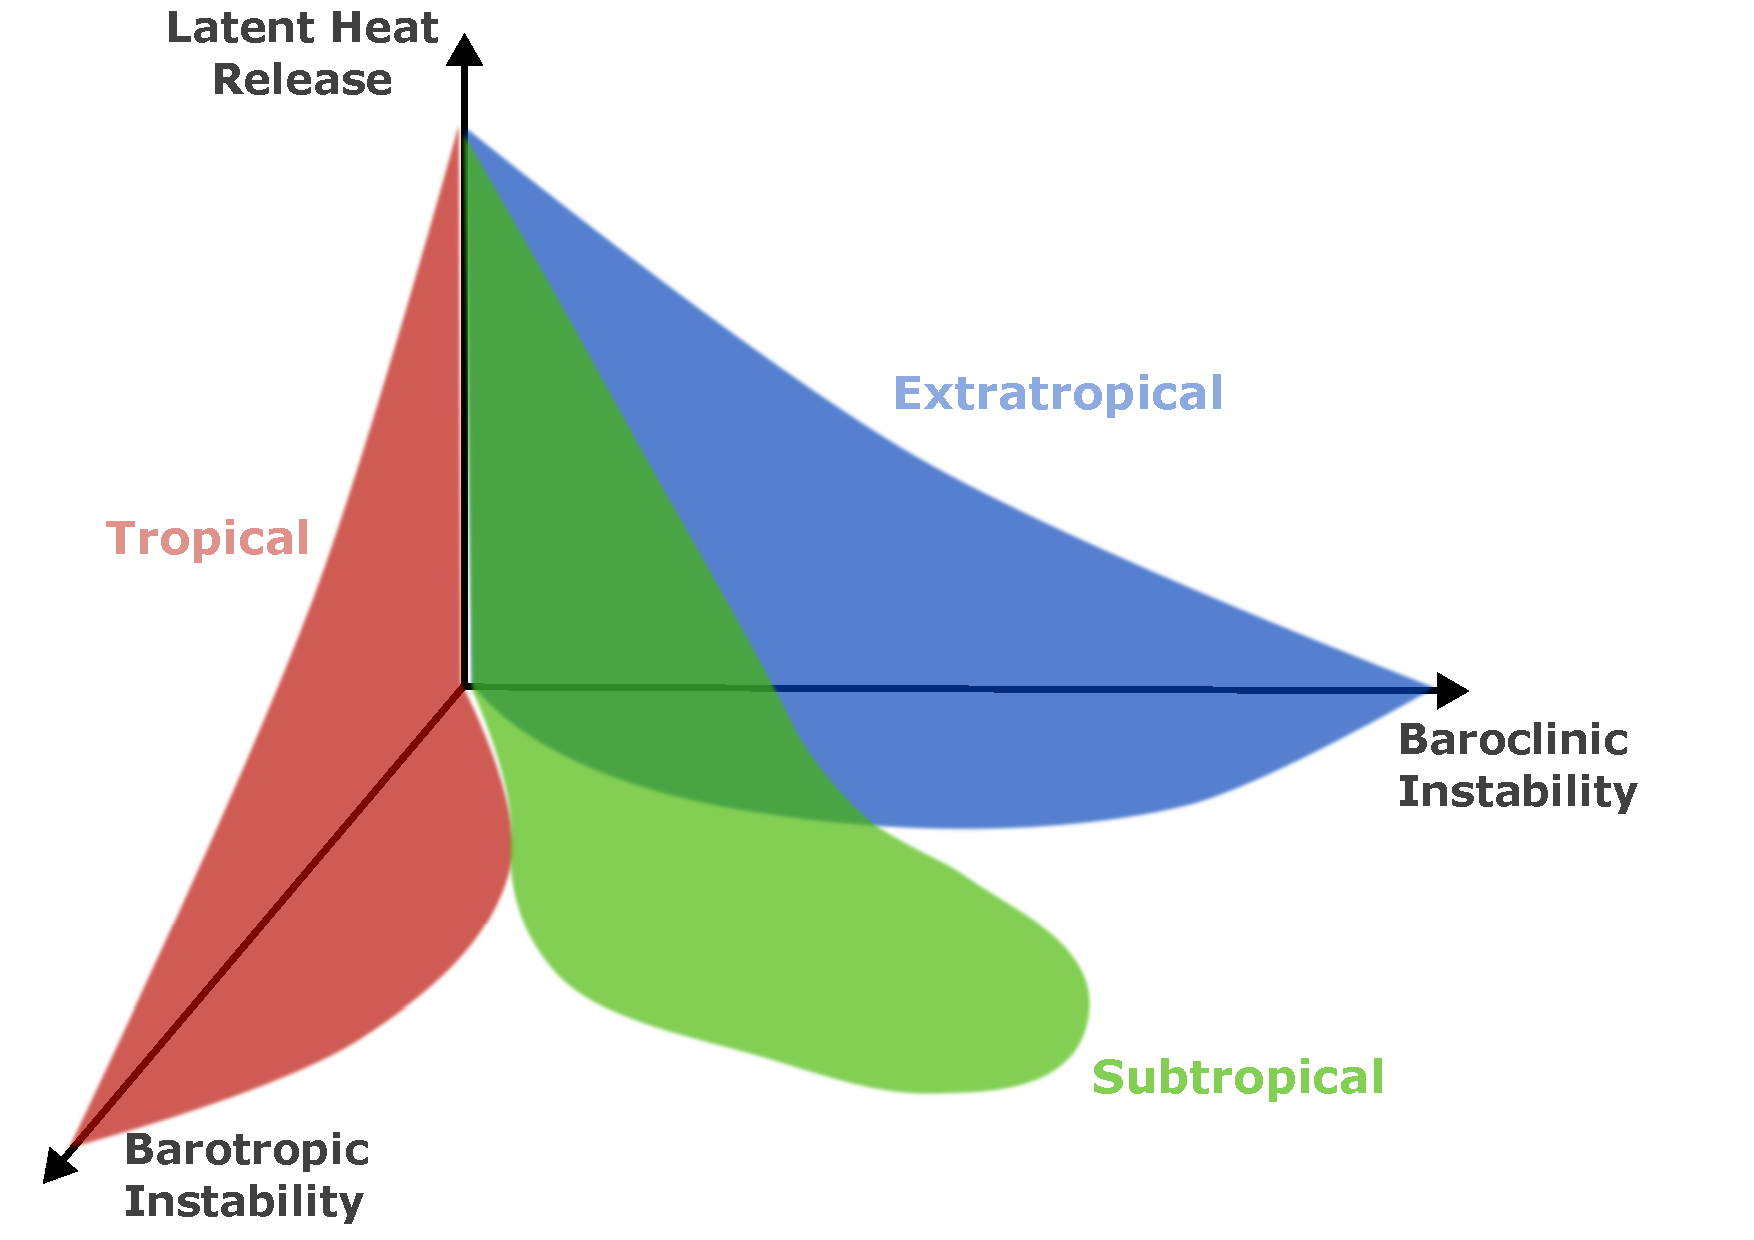
\includegraphics[width=0.9\columnwidth,angle=0]{fig/instabilities_cyclones_types.pdf}
\caption[Conceptual Model: Instabilities and Types of Cyclones]{Proposed conceptual model correlating atmospheric destabilization mechanisms with cyclone types. Each axis within the three-dimensional schema represents a different process of atmospheric destabilization, allowing the categorization of cyclone types across the spectrum. Adapted from \citet{silva_dias_catarina_2004}.}
\label{concecputal_view_instabilities}
\end{center}
\end{figure}

\subsection{Final Causes}

Final causes delve into the purpose or ultimate reason for the existence of something, offering insights into the "why" behind its occurrence. For instance, the final cause of a table is to serve as a platform for activities such as writing, eating, or working. When considering cyclones, their final cause could be viewed as the facilitation of heat and moisture redistribution within the atmosphere, thus playing a crucial role in maintaining global climatic equilibrium and acting as a mechanism for dissipating excess heat.

The Earth's climate system is fundamentally driven by solar radiation, while simultaneously losing heat through infrared radiation emitted into space. The unequal distribution of solar radiation, exacerbated by the tilt of the Earth's axis, results in energy surpluses in equatorial regions and deficits in polar areas. This differential heating prompts the formation of warm air masses near the equator and cold air masses in polar regions, instigating atmospheric circulation as an effort to achieve thermal equilibrium, a state that remains elusive due to ongoing differential heating between tropical and polar zones.

Historical and recent advancements in atmospheric science have underscored the significance of general atmospheric circulation in climate dynamics \citep{lorenz1967nature, hadley1735vi, stull2015practical, schneider2006general}. The Hadley Cell emerges as a critical response to the disparity in solar radiation received at the equator compared to the poles (Figure \ref{global_circulation}). Warmed air rises near the equator, creating low-pressure zones at the surface and high pressure aloft. This ascending air, replaced by cooler air from higher latitudes, moves poleward at elevated altitudes due to mass conservation. The conservation of angular momentum is crucial as this air, moving away from the equator (where surface rotational speed is maximum), must increase its eastward velocity as it approaches the poles. This dynamic leads to the formation of subtropical jet streams around 30° latitude. The Polar Cell, integral to high-latitude atmospheric circulation, is driven by the thermal contrast between the poles and regions at 60° latitude. This temperature difference induces opposing north-south pressure gradients, generating equatorward winds that, due to the Coriolis force, become polar easterlies. At higher levels, winds flow poleward but are deflected eastward, forming an upper-level westerly flow around the polar low, thus completing the Polar Cell circulation.

\begin{figure}[h!]
\begin{center}
\setcaptionmargin{1cm}
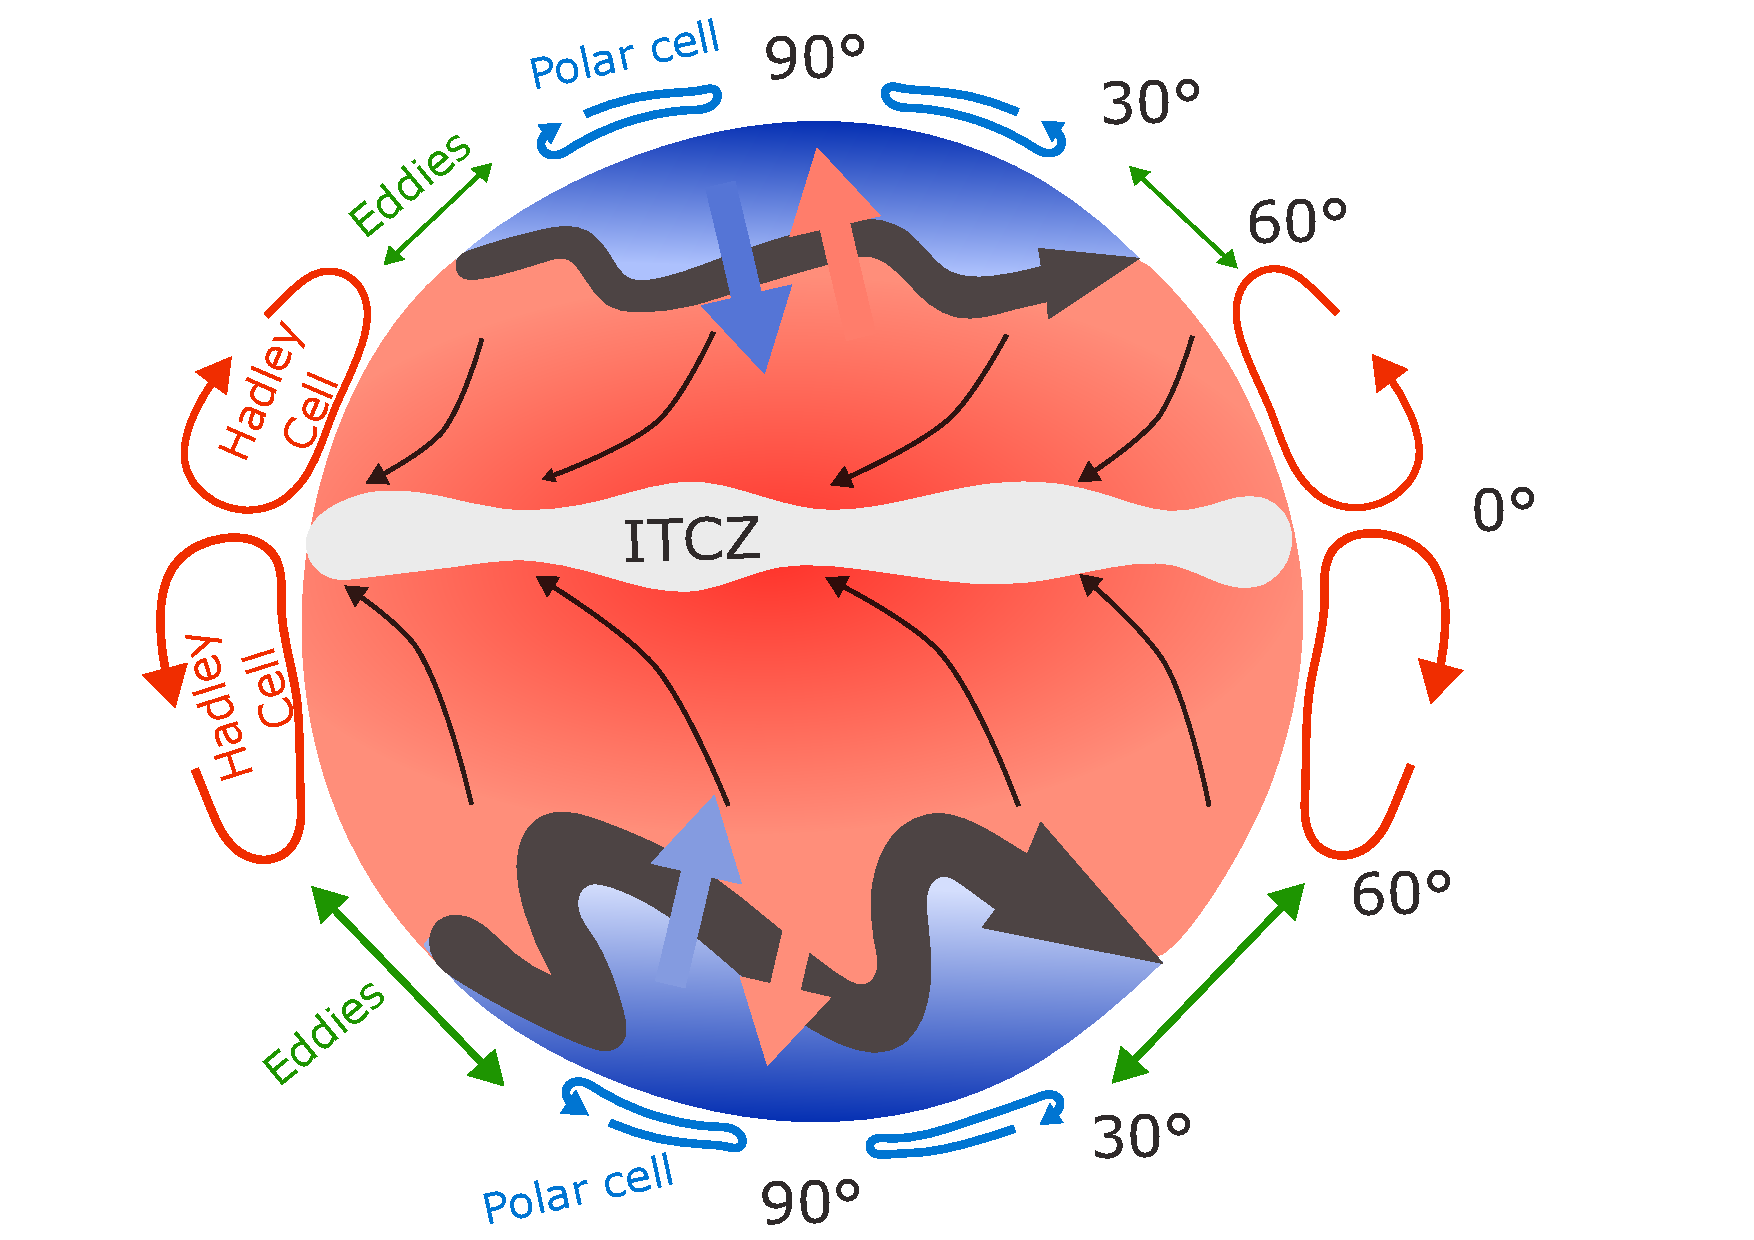
\includegraphics[width=0.9\columnwidth,angle=0]{fig/global_circulation.pdf}
\caption[Global Circulation]{Representation of the global circulation pattern, showing the Hadley Cell circulation prominent at low latitudes, the transport of momentum and heat by eddies at mid-latitudes, and the polar cell circulation at high latitudes. Inspired by \citet{stull2015practical}.}
\label{global_circulation}
\end{center}
\end{figure}


Together, the Hadley and Polar Cells underscore a comprehensive circulation pattern that transports warm air and angular momentum from the equator towards the poles and vice versa, facilitating Earth's energy balance. Although initially conceptualized as symmetrical circulations extending from the equator to the poles, subsequent research has emphasized the pivotal role of large-scale eddies in heat and angular momentum transfer \citep{schneider2006general}. These eddies, critical to atmospheric dynamics, emerge due to baroclinic zones in mid-latitudes and are intrinsic to the structure and function of the Ferrel Cell in mid-latitudes\citep{held1999macroturbulence,schneider2006general}. Arising from mid-latitude baroclinic zones, they are indispensable to the Ferrel Cell's operation, influencing wind patterns across latitudes and enhancing heat transfer between the tropics and poles \citep{stull2015practical, held1999macroturbulence}.

Due to their relatively small scale compared to extratropical cyclones, tropical cyclones are not directly associated with the three-cell model of global circulation. They arise in regions of low baroclinicity, where thermal contrasts are minimal, relying instead on the atmosphere's ability to generate energy from internal heat sources. These sources are largely the warm temperatures of tropical oceans and the air above them \citep{palmen1969atmospheric}. Often conceptualized as a Carnot heat engine (Figure \ref{carnot_cycle}), tropical cyclones draw heat from the ocean surface—primarily through the latent heat of vaporization—and release it into space via longwave radiation \citep[e.g.,]{emanuel1987dependence,ozawa2015thermodynamics,wang2022tropical}. The cyclone's intensity depends on the efficiency of this heat engine, which is determined by the temperature difference between the heat source (ocean) and sink (upper atmosphere). Friction, especially near the ocean surface within the boundary layer, plays a crucial role by causing energy loss that can lessen wind speeds and alter angular momentum, impacting the cyclone's energy conversion efficiency.

\begin{figure}[h!]
\begin{center}
\setcaptionmargin{1cm}
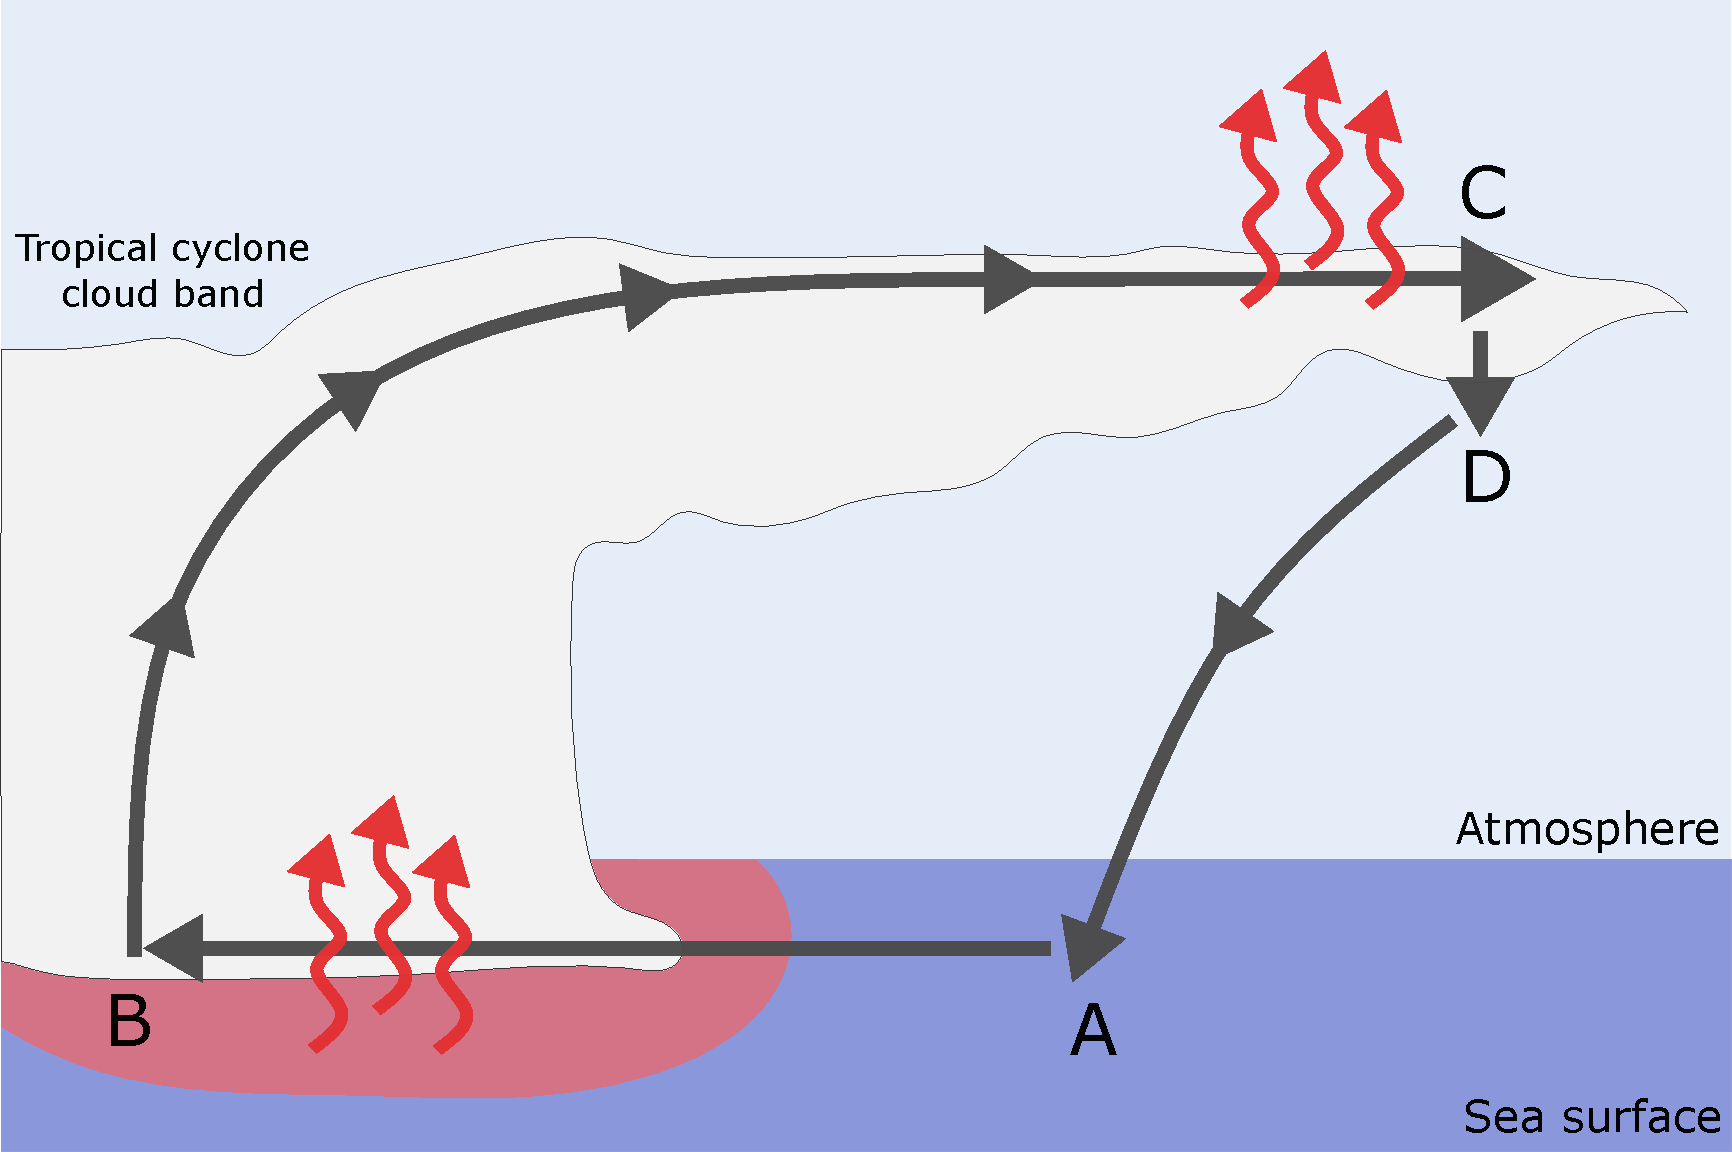
\includegraphics[width=0.9\columnwidth,angle=0]{fig/carnot_cycle.pdf}
\caption[Tropical Cyclone as a Carnot Cycle]{Diagrammatic Representation of a Tropical Cyclone as a Carnot Heat Engine. The process begins with isothermal inflow (A-B) at the surface, drawing energy from warm ocean waters into the cyclone's core. This stage is succeeded by the upward movement of air (convection) and outward flow just below the tropopause, characterized by radiative cooling and energy loss (B-C). Subsequently, cooled air descends away from the cyclone's center (C-D) and cycles back towards the cyclone, completing the circuit (D-A). Adaptation based on the COMET Program.}
\label{carnot_cycle}
\end{center}
\end{figure}


We can see then that tropical cyclones serve to dissipate excess heat in the tropics, utilizing oceanic heat to fuel the system while dissipating energy through radiation at the upper levels or friction at the surface. Given this model's applicability, \citet{emanuel1987dependence} predicted that rising atmospheric $CO_2$ levels would lead to more intense tropical cyclones in the future. Recent climate models suggest an increase in tropical cyclone intensity, though there's no global consensus on frequency changes \citep{knutson2010tropical,walsh2004tropical,walsh2016tropical,walsh2019tropical}. As discussed in Section \ref{efficient_causes}, understanding tropical cyclone development remains a significant scientific endeavor, complicating precise predictions of their response to climate change and their regulatory effect on climate.

In exploring subtropical cyclones, much remains to be discovered. The global distribution of cyclonic activity exhibits a bimodal pattern, with tropical cyclones forming in tropical regions and extratropical cyclones in mid-latitudes, leaving subtropical areas relatively calm in terms of cyclonic development \citep{yanase2014parameter}. It's speculative—emphasis on "speculate"—to suggest that subtropical systems share the final causes of their tropical and extratropical counterparts, acting to erase thermal gradients by redistributing heat globally or dissipating excess heat. However, subtropical cyclones might perform these functions under hybrid environmental conditions, possibly moderating gradients in regions with an abundance of heat. Ongoing research into subtropical cyclones promises to provide further clarity on their impact on global circulation patterns and their role within the broader climatic system.

\subsection{Summary}

This section has explored the Aristotelian causes as they pertain to cyclones, comparing the various types—extratropical, tropical, and subtropical—while also acknowledging the existence of other cyclonic phenomena like warm seclusions and polar lows. For succinctness, the discussion primarily centered on the main types, suggesting that cyclonic systems form a continuum: extratropical systems at one end, tropical cyclones at the other, and subtropical systems exhibiting hybrid characteristics.

Initially, we discussed that cyclones' material causes are linked to the air masses constituting them. Extratropical cyclones are associated with cold cores throughout the troposphere, whereas tropical cyclones are characterized by warm cores. Subtropical cyclones, however, display warm cores at the surface and cold cores at higher tropospheric levels.

Regarding formal causes, the cyclones differ in structure. Extratropical cyclones, identified by their frontal features, show asymmetry. Tropical cyclones, described as symmetric, feature convection bands spiraling the central eye. Subtropical cyclones, meanwhile, may present a range of spatial configurations, neither fully asymmetric nor symmetric.

Efficient causes, the dynamic mechanisms behind cyclone development, vary. Extratropical cyclones are primarily driven by baroclinic instability, a comprehensive mechanism underlying their formation. Tropical cyclone genesis and intensification lack a unified theoretical model, with current theories suggesting that barotropic instability in tropical waves—coupled with diabatic processes like latent heat release—might describe their development. Subtropical systems, given the incipient state of research, are speculatively linked by the author to both baroclinic and barotropic instabilities, with diabatic heat playing a role.

The final causes reflect cyclones' contributions to global circulation. Extratropical cyclones are recognized for redistributing heat, mitigating temperature gradients in mid-latitudes. Tropical cyclones, functioning as thermal engines, dissipate excess heat in tropical regions. The role of subtropical cyclones in the climate system remains speculative; they are hypothesized to simultaneously embody the functions of the other two types.

One important feature noted is that most classifications adopted for cyclone classification are based on \citet{hart2003cyclone} diagrams that objectively distinguishes these systems based on their material and formal causes. Although much knowledge exists regarding the efficient and final causes of tropical and especially extratropical systems, such objective criterion for these causes is still lacking. The current research proposes such objective classification procedure in the hopes of aiding the investigation of such causes related to cyclonic systems. 

A notable point is the reliance on \citet{hart2003cyclone}'s diagrams for cyclone classification, objectively differentiating systems by their material and formal causes. While extensive knowledge exists on the efficient and final causes of tropical and particularly extratropical systems, a clear criterion for these causes is absent. This work proposes an objective classification procedure to aid in investigating cyclonic systems' related causes.

\section{Cyclones in South America}\label{SA_cyclones_climatology}

This section transitions to examining cyclonic phenomena within South America, with a particular emphasis on systems originating in or adjacent to this region. While previous sections have provided a comprehensive overview of various cyclone categories, their structures, formation mechanisms, and roles in atmospheric circulation, here we delve into cyclonic systems that have genesis in South America or its neighboring oceanic regions. Although systems originating along the western coast of South America are noted \citep[e.g.,]{crespo2023assessment}, our primary focus is on cyclones forming in the southern and eastern sectors of South America and the Southeastern Atlantic region. These systems significantly influence the regional climate, particularly in South and Southeastern Brazil \citep[e.g.]{de2022hybrid,reboita2010regimes}, and can cause extreme weather events \citep[e.g.]{cardoso2022synoptic,de2021ocean,gramcianinov2020extreme}. From this point on, we refer to this region encompassing the Southeastern Atlantic and the adjacent South American region as SESA.

\subsection{Climatological aspects}

The first cyclone climatology for SESA region was performed by \citet{gan1991surface}, utilizing sea level pressure data from surface charts spanning a decade. Despite methodological constraints, the authors identified two primary cyclogenesis regions: one over Uruguay and another in Southeast Argentina, with the latter being more active in austral summer and the former in winter. They hypothesized that the cyclogenesis in these regions was driven by baroclinic instability of the westerlies and lee cyclogenesis—cyclogenesis influenced by the interaction between baroclinic disturbances and topography \citep{gan1994influence,tibaldi1980orographically}.

Later studies, employing automated techniques to detect cyclones' minimum central pressure, validated the cyclogenesis regions identified by \citet{gan1991surface} \citep{simmonds1999southern,simmonds2000mean,mendes2010climatology}. Meanwhile, analyses based on relative vorticity fields, as opposed to minimum central pressure, found a third significant cyclogenesis area near Southeast Brazil \citep{hoskins2005new,sinclair1995climatology,reboita2010south,gramcianinov2019properties}. The shift towards relative vorticity for cyclone tracking, as discussed by \citet{hoskins2002new,sinclair1994objective}, offers several technical advantages. In mid-latitudes, the background pressure gradient's intensity can foreshadow closed isobars in developing cyclones, making it challenging to detect cyclones until they intensify or reach higher latitudes. Thus, employing relative vorticity enables the identification of weaker and faster-moving systems, as well as cyclones in their nascent stages, when closed isobars might not yet be evident.

In the SESA region, previous research has successfully identified three key areas of cyclogenesis, and this current study will adopt the nomenclature established by \citet{gramcianinov2019properties} for consistency and clarity. The ARG region, situated in Southeast Argentina, emerges as the most active, with a relatively steady cyclogenesis rate throughout the year, though it peaks during the austral summer \citep{crespo2021potential,gramcianinov2019properties,reboita2010south}. The LA-PLATA region, over the La Plata River basin, ranks second in genesis density, displaying heightened activity in the austral winter \citep{crespo2021potential,gramcianinov2019properties,reboita2010south}. It's noteworthy that \citet{reboita2010south} identified the LA-PLATA region along the Uruguayan coast rather than over the continent, influenced by the application of a continental mask in cyclone tracking, which biases detection towards maritime regions. The final region, SE-BR, located near the Southeastern Brazilian coast, records the fewest genesis events, with a significant increase in activity during the austral summer compared to winter \citep{reboita2010south,gramcianinov2019properties,crespo2021potential}. Figure \ref{genesis_regions} summarises these findings. 

\begin{figure}[h!]
\begin{center}
\setcaptionmargin{1cm}
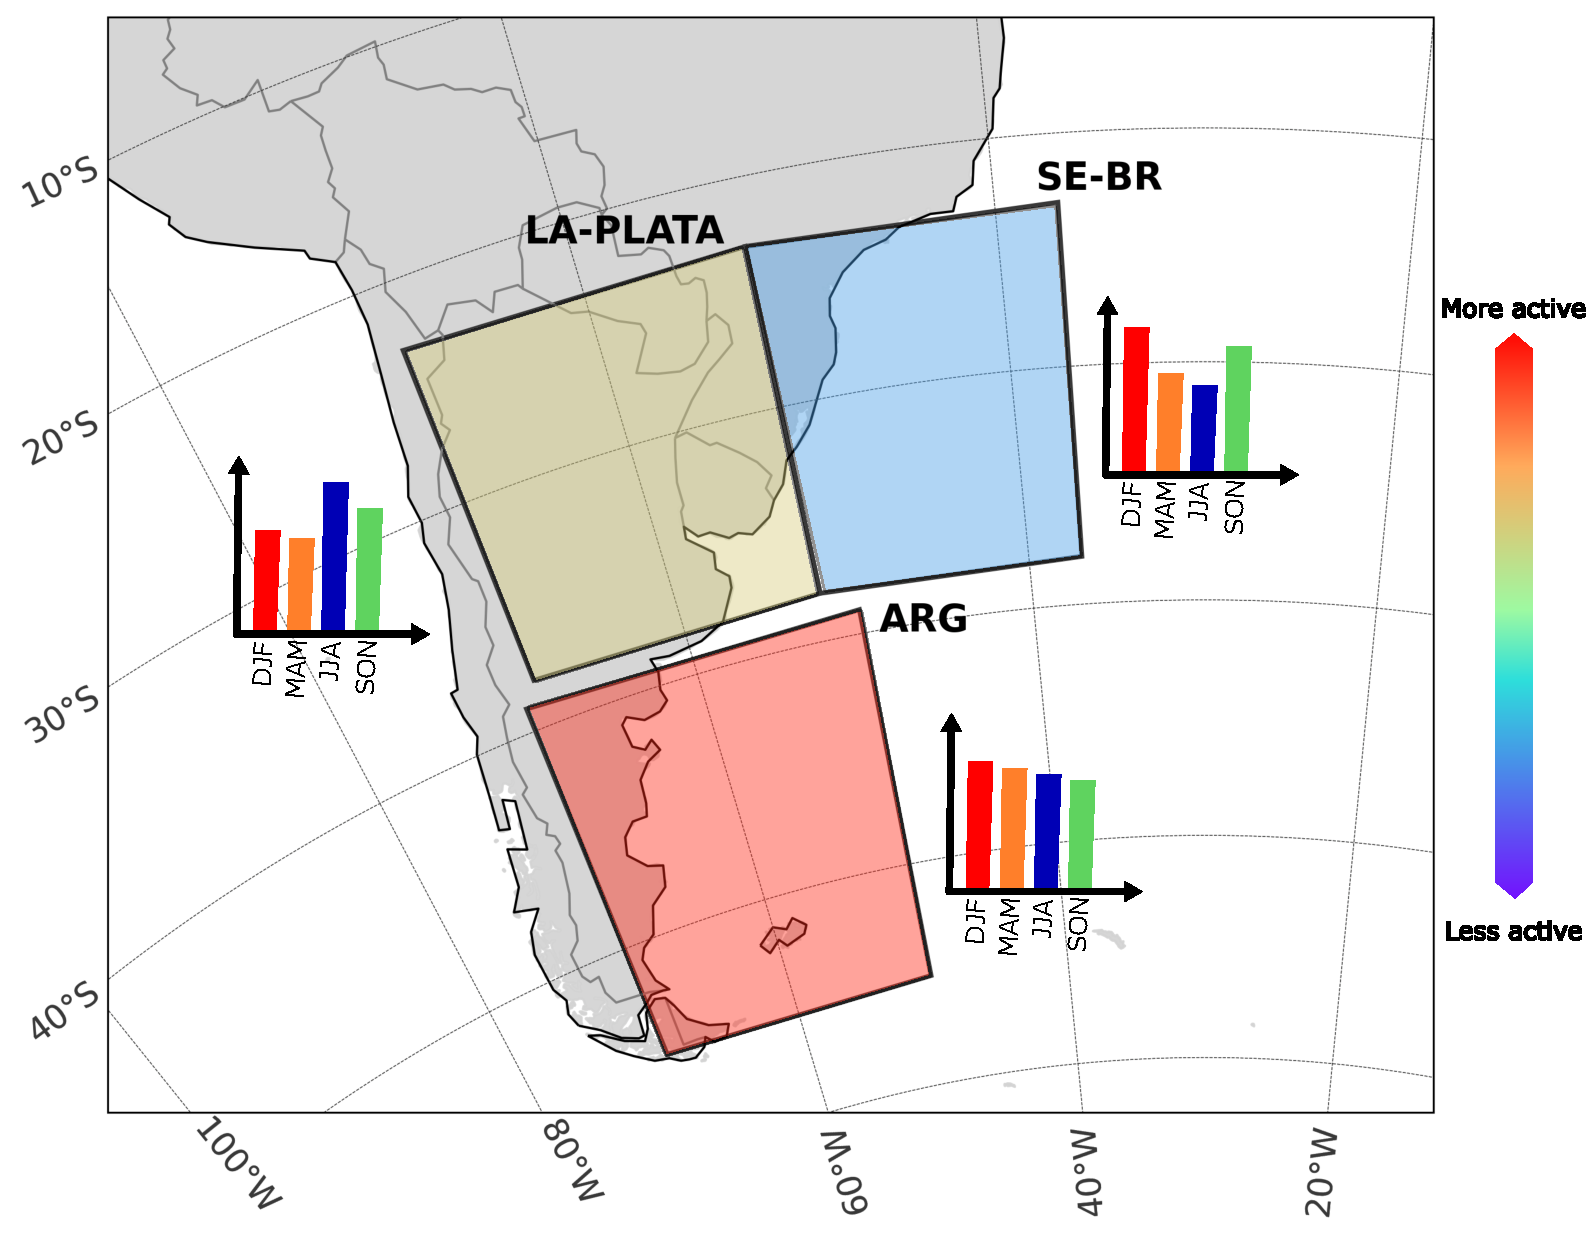
\includegraphics[width=0.9\columnwidth,angle=0]{fig/genesis_regions.pdf}
\caption[Cyclogenesis regions in the South Atlantic]{Illustrative mapping of cyclogenesis activity within the South American/Southeastern Atlantic (SESA) region, categorized into three primary genesis areas: ARG (Southeast Argentina), LA-PLATA (La Plata River basin), and SE-BR (Southeastern Brazilian coast). The diagram highlights the cyclogenesis frequency and seasonal patterns in each region, with a visual scale indicating activity levels from more active to less active.}
\label{genesis_regions}
\end{center}
\end{figure}


\subsection{Genesis mechanisms}\label{genesis_mechanisms}

The majority of systems in SESA region are extratropical \citep{marrafon2022classificaccao}, thus baroclinic instability serves as the primary genesis mechanism across all regions, as discussed in Section \ref{efficient_causes}. However, each region is also influenced by secondary mechanisms. Notably, all regions lie on the lee side of the Andes, where baroclinic development of troughs crossing the mountain range can prompt surface cyclogenesis \citep{gan1994influence,vera2002cold,hoskins2005new,gramcianinov2019properties}. Additionally, downstream development, marked by system decay on the Andes' upslope and regeneration on the downslope facilitated by vortex stretching over the mountain barrier, is observed \citep{hoskins2005new}. 

Subsequent analyses by \citet{gramcianinov2019properties} and \citet{crespo2021potential} delve into the specific genesis mechanisms for each cyclogenesis region. Their findings, synthesized in this section, compare summer and winter mechanisms, as transitional seasons typically exhibit intermediate characteristics \citep{gan1991surface,hoskins2005new,gramcianinov2019properties,crespo2021potential}.

In both seasons, cyclones in ARG region tend to follow a traditional baroclinic development pathway, heavily influenced by low level cold advection \citep{gramcianinov2019properties}. This advection is crucial in reducing static stability, due to the contrast between the warmer surface and cold air aloft, thereby facilitating cyclogenesis. The cyclogenesis position relative to the jet stream provides upper-level support, either at the poleward exit during summer or the equatorward entrance during winter \citep{crespo2021potential}. During summer, a slightly more baroclinic environment and more pronounced potential vorticity anomalies promote conditions favorable for ascending vertical movements \citep{crespo2021potential}.

Cyclone development in the LA-PLATA region is initially driven by moisture transport from the South American low-level jet on the eastern slope of the Andes and from the South Atlantic Subtropical High towards the southeastern coast \citep{gramcianinov2019properties}. This transport feeds cyclone development with warm, moist air, promoting low-level instability. Furthermore, cyclogenesis in this region is influenced by potential vorticity anomalies in both summer and winter \citep{crespo2021potential}. The area is positioned beneath the equatorial entrance of a jet streak in both seasons, with a slightly more pronounced baroclinic environment in winter \citep{crespo2021potential}.

During summer, cyclogenesis in the SE-BR region is significantly influenced by the transport of warm and moist air from the tropics, associated with the South Atlantic Convergence Zone (SACZ) \citep{gramcianinov2019properties}. This process contributes to cyclogenesis through diabatic heating and convective processes. In winter, upper-level forcing becomes more prominent, with baroclinic conditions intensified by the presence of strong temperature gradients and jet stream dynamics \citep{gramcianinov2019properties}. Moreover, during summer, cyclogenesis occurs in a more barotropic environment, with the jet stream significantly displaced from the genesis region, and is highly influenced by high-level potential vorticity anomalies \citep{crespo2021potential}. Conversely, in winter, cyclogenesis occurs beneath the equatorial entrance of a jet streak in a more baroclinic environment compared to summer, influenced by low-level potential vorticity anomalies \citep{crespo2021potential}.

\subsection{Subtropical cyclones}

It was only after \citet{hart2003cyclone} work that the scientific community started to take a closer look to subtropical cyclones.  It wasn't until about 20 years ago that the first detailed climatology for subtropical cyclones in the South Atlantic was conducted by \citet{evans2003objective}. This study uncovered an average occurrence of roughly one subtropical cyclone per year in the region, with a relatively uniform distribution across seasons. Notably, subtropical cyclogenesis was found to occur in diverse environments: genesis in the open ocean primarily involves Rossby wave breaking, similar to systems in the North Atlantic, whereas coastal genesis is often related to lee cyclogenesis, influenced by the warmer sea surface temperatures of the Brazilian Current, which create conducive conditions for subtropical cyclone formation.

More recently, \citet{gozzo2014subtropical} introduced modifications to the criteria used by \citet{evans2003objective}, aiming to capture weaker and shallower systems in their analysis. This adjustment led to the identification of an average of 7 cyclones per year, a significant increase from the findings of the previous study. \citet{gozzo2014subtropical} emphasized the subtropical cyclones' lower traveled distance and displacement speed compared to their extratropical counterparts, allowing them more time to interact with the unstable conditions that facilitated their genesis and to exert greater impact on the South American coastal zone.

Moreover, \citet{gozzo2014subtropical} noted distinctions in seasonal activity, with a peak during summer but stronger systems occurring in autumn. The Southeastern Brazil region (SE-BR) emerged as the predominant genesis area, with over a third of the cyclones developing there exhibiting hybrid characteristics. These systems typically originate from upper-level potential vorticity anomalies and divergence within a low-shear environment. At lower levels, warm and moist air advection, primarily from the subtropical high, is crucial for their formation. During summer, an additional moisture source from the tropics is also significant. Also, the authors used numerical simulation for demonstrating the importance of local latent heat fluxes for the systems develoment.

\citet{gozzo2017climatology} reinforced the findings of \citet{gozzo2014subtropical}, confirming the role of moisture fluxes in the formation of subtropical cyclones in the SE-BR region. They highlighted that moisture transport from the subtropical high is particularly crucial during the summer months when it shifts closer to the Brazilian southeastern coast. The reduced number of genesis events observed in the winter can be attributed to the diminished strength of this moisture transport. In contrast, during autumn, transient high-pressure systems serve as the primary source of moisture. Moreover, through numerical simulations, the authors demonstrated the significance of local latent heat fluxes in the development of these systems.

Subtropical cyclones in the South Atlantic remain an area ripe for exploration due to their relatively sparse coverage in scientific literature. From the limited climatologies available, and the few study cases \citep[e.g.]{reboita2018key,reboita2022shapiro,dias2011energy} it is evident that the formation of these systems is closely linked to Rossby wave breaking and are fueled by both local and non-local latent heat fluxes. However, the door remains open for more comprehensive studies to explore the their dynamics, climatological impacts, and the potential influence of broader atmospheric and oceanic processes on their formation.


\subsection{Tropical cyclones}

Historically, it was believed that the SESA was not conducive to Tropical Cyclone formation due to insufficiently high sea-surface temperatures and relatively strong vertical wind shear, a perspective dating back to \citet{gray1968global}, which identified the South Atlantic as the sole oceanic basin without such systems. This view was upended by Hurricane Catarina in 2004, the first recorded hurricane in the South Atlantic, challenging previous assumptions despite some evidence of weak tropical cyclones in the region before the satellite era \citep{dasilva2004ciclone}.

Catarina, which originated from an extratropical system near the southeastern Brazilian coast, underwent a tropical transition and made landfall in Southern Brazil \citep{pezza2005first}. The system's trajectory and development were significantly influenced by unique environmental conditions, including a dipole-blocking pattern in the upper atmosphere, guiding the system back toward Brazil over relatively cool sea surface temperatures (SSTs) of around 25°C \citep{mctaggart2006analysis}. This development over cooler SSTs was facilitated by a unique combination of extreme blocking conditions, low wind shear favored by an extreme positive phase of the Southern Annular Mode \citep{pezza2005first,pezza2009climate}, and latent heat release from air-sea interactions. Strong interactions with sub-superficial warm waters by Ekman pumping led to the upwelling of isotherms and mixed layer waters, allowing for a significant air-sea temperature gradient and vigorous heat exchange between the ocean and atmosphere, fueling the system through latent heat release \citep{vianna2010interactions,pereira2010new}.

Hurricane Catarina, while a landmark event, did not originate from a purely tropical process; it was a baroclinic cyclone that underwent tropical transition. This distinction was pivotal until the emergence of a system near Brazil's Northeast oceanic region in 2019, reported as the first instance of pure tropical cyclogenesis in the South Atlantic. This system, named Iba, marked a significant departure from previous understandings of cyclonic activity in the region \citep{reboita2021iba}. Additionally, research on subtropical cyclone Anita in March 2010 suggested its potential for tropical transition under warmer sea surface conditions and without interference from a neighboring extratropical cyclone \citep{dias2011energy,reboita2019subtropical}. In March 2024, another system named Akará, originating near Southeastern Brazil and featuring eye-like characteristics and a symmetric form, ignited discussions regarding its potential classification as a tropical cyclone, although a detailed examination of its characteristics is pending.

The sporadic nature of these systems in the SESA region precludes the formation of a comprehensive tropical cyclone climatology. While there is some conjecture about the influence of climate change on the emergence of these systems \citep[e.g.,]{pezza2005first,mctaggart2006analysis,pezza2009climate,pereira2010new}, establishing a direct connection between recent tropical cyclone occurrences in SESA and global climatic shifts remains elusive. The rarity of such events continues to challenge researchers, suggesting a complex interaction between regional climatic conditions and broader atmospheric patterns influenced by climate change.

\section{Life cycle of extratropical cyclones: objective classification procedures}

This section explores lifecycle and classification procedures for extratropical cyclones, building upon conceptual models and evolution patterns discussed in Sections \ref{formal_cause} and \ref{efficient_causes}. These models, derived from case studies and numerical simulations, seek to generalize cyclone development phases due to the absence of standardized methods for analyzing distinct lifecycle stages across extensive datasets. Herein, we introduce an automated approach for detecting the lifecycle of cyclones, thereby advancing the discussion on objective classification methodologies for these atmospheric phenomena.

The Polar Front Theory, as detailed by \citet{bjerknes1922life}, was among the first to describe the lifecycle of extratropical cyclones, delineating distinct phases based on structural transformations and large-scale dynamics. Nonetheless, \citet{shapiro1990fronts} later argued that not all cyclones adhere strictly to the progression outlined by Bjerknes, proposing an alternative model that complements the original theory. These developmental models, including their respective stages, are elaborated in Section \ref{formal_cause} and illustrated in Figure \ref{cyclone_models}. While these descriptions offer detailed insights into the structural changes cyclones undergo, they fall short of directly associating each phase with specific atmospheric variables in a way that allows for algorithmic detection and statistical and/or spatial analysis.

\citet{whittaker1984northern} conducted one of the earliest cyclone climatology studies, identifying cyclogenesis regions based on the formation of the first closed isobar. This definition has been widely used since \citep[e.g]{gramcianinov2019properties,trigo2006climatology,hoskins2005new,simmonds2000mean}. \citet{whittaker1984northern} also defined cyclone intensification as the rate of sea level pressure deepening, a definition echoed and expanded upon by later studies through metrics like relative vorticity growth rate \citep{grise2013intraseasonal,gramcianinov2019properties,hoskins2005new} and the baroclinic Eady growth rate \citep{pinto2005sensitivities}. However, Whittaker's study lacked a comprehensive method for classifying cyclone evolution.

A classification of the developmental phases throughout the life cycle of cyclones was conducted by \citet{evans2003objective}, with a particular focus on tropical cyclones undergoing extratropical transition. This study explored the structural evolution of such systems, employing a classification framework grounded in the environmental parameters outlined by \citet{hart2003cyclone}. The authors partitioned the life cycle of the cyclones into two main phases: one preceding and the other following the peak intensity of the tropical cyclone. This demarcation enabled a detailed analysis of the transformation these cyclones undergo from their genesis as tropical entities to their eventual extratropical characteristics.

\citet{gray2006classifying} implemented the classification scheme originally proposed by \citet{deveson2002classification}, as detailed in Section \ref{efficient_causes}, to study the climatology of Northern Atlantic extratropical cyclones. Their analysis focused on the separation between the upper-level trough and the lower-level cyclone throughout the cyclones' intensification periods, which were identified when the cyclones' central relative vorticity surpassed a specified threshold. While this approach proved beneficial for classification purposes, it overlooked the exploration of dynamical forcing during the development of cyclones. Furthermore, the rationale behind the selected threshold value, including its potential applicability across various scenarios, remained unexplored.

Building upon the foundation laid by \citet{gray2006classifying}, \citet{dacre2009spatial} delved into the environmental forces influencing the evolution of different types of cyclones. To achieve a granular understanding of variations throughout the cyclones' life cycle, they segmented the cycle at the juncture of maximum relative vorticity. This segmentation delineated the period leading up to this juncture as the intensification stage and the subsequent period as the decaying stage. Additionally, by categorizing cyclones based on their overall lifespan, the study facilitated the identification of specific areas prone to cyclone intensification and the environmental characteristics predominant in those regions.

\citet{rudeva2007climatology} delved into the study of changes in the radius of cyclones throughout their life cycle, introducing the concept of "nondimensional cyclone lifetime." This methodology facilitates the comparison of different stages of cyclone development by normalizing their lifespan to a uniform scale, achieved by dividing the current time step within the system's life cycle by its total duration. Similar apporaches were employed by \citet{booth2018extratropical} and \citet{schemm2018during}. Specifically, \citet{booth2018extratropical} focused on analyzing precipitation rates through the cyclone life cycle, identifying the cyclones' peak dynamical strength with the point of maximum relative vorticity. Concurrently, \citet{schemm2018during} applied normalization to the cyclone life cycles using the duration from genesis to lysis, thereby examining the periods when the systems were associated with frontal structures.

\citet{trigo2006climatology} explored the spatial distribution of cyclogenesis (i.e., the initial detection point of each low-pressure system), cyclolysis (the final detected position), and the locations where these systems attained their minimum central pressure. Similarly, \citet{bengtsson2009will}, albeit not explicitly defining developmental stages, observed distinguishable phases centered around the maximum intensity of the system, characterized as the period when maximum central relative vorticity is reached. Meanwhile, \citet{azad2014vorticity,azad2014vorticity2} dissected the cyclone life cycle into distinct stages, identifying the mature phase as the period during which geostrophic vorticity experiences its most rapid increase, with the incipient stage occurring beforehand. Moreover, they categorized the life cycle of a cyclone based on the maximum geostrophic vorticity attained; the time leading up to this peak is labeled as the intensification stage, while the subsequent period is known as the decaying stage. 

The diverse methodologies highlighted in the literature offer a range of objective criteria for delineating the lifecycle of extratropical cyclones, each linked to the temporal dynamics of specific atmospheric variables. Commonly, cyclone genesis is identified at the algorithm's first detection, with intensification and decay phases typically defined by changes in central pressure or, when using relative vorticity for tracking, by the increase (intensification) or decrease (decay) of vorticity in the Northern Hemisphere. The peak of the system's intensity is often marked as the point of maturity, while lysis is recognized at the algorithm's final detection of the system.  A schematic illustration of this lifecycle, emphasizing the use of relative vorticity at the 850 hPa isobaric level ($\zeta_{850}$) for cyclone detection, is depicted in Figure \ref{cyclone_life_cycle}.

\begin{figure}[h!]
\begin{center}
\setcaptionmargin{1cm}
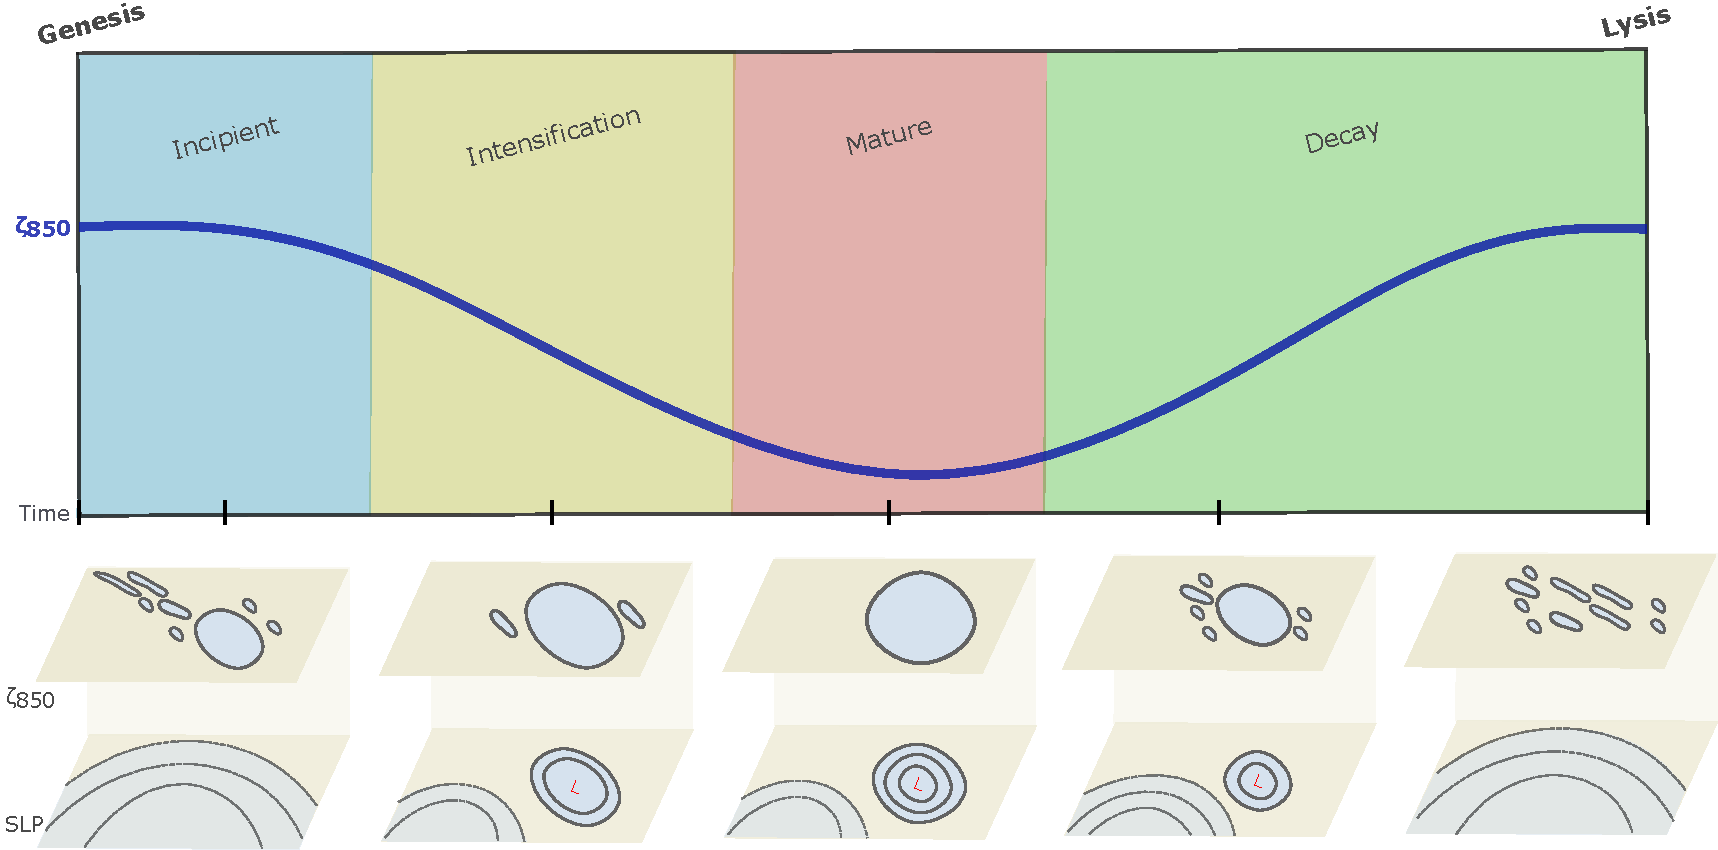
\includegraphics[width=0.9\columnwidth,angle=0]{fig/cyclone_life_cycle.pdf}
\caption[Extratropical Cyclone Life Cycle]{Schematic representation of an extratropical cyclone's life cycle, depicted through the relative vorticity field at the 850 hPa isobaric level ($\zeta_{850}$). The central figure displays the temporal progression of central $\zeta_{850}$ at the cyclone's core across various phases. The bottom figures illustrate the evolution of the $\zeta_{850}$ field and sea level pressure (SLP) spatial distributions during each phase.}

\label{cyclone_life_cycle}
\end{center}
\end{figure}

Despite these advancements, several limitations persist in current approaches. First, the initial phase of cyclone development, where the system is present but not yet fully formed, is often overlooked. In such instances, a cyclone may exhibit closed central relative vorticity without corresponding closed isobars at sea level pressure \citep[e.g.]{sinclair1995climatology}. Second, defining cyclone maturity as merely the point of maximum intensity overlooks the broader period during which atmospheric dynamics illustrates the cyclone's evolution. Finally, characterizing all stages between genesis and maturity as intensification, and those between maturity and lysis as decay, presupposes a singular, linear progression of these stages. This assumption fails to account for the potential complexity of cyclone lifecycle stages, including the possibility of multiple intensification and decay phases.

The ability to discern the distinct life cycle phases of cyclones is crucial for several reasons. As highlighted in Section \ref{SA_cyclones_climatology}, most climatologies currently focus on either the entirety of a cyclone's life cycle or specific points, such as its genesis or lysis. Enhanced techniques for dissecting a cyclone's life cycle could unlock the potential for more granular analyses of the processes and environmental dynamics associated with different stages of cyclone development. For example, while the initial baroclinicity associated with extratropical cyclones is well-documented, the environmental shifts that trigger their cessation of intensification remain less understood. Case studies have shed light on these aspects, but comprehensive testing under climatological conditions is yet to be conducted.

By identifying the environmental conditions pertinent to various stages of cyclone development, researchers can leverage climate change projections to assess potential future shifts in these conditions. Moreover, given the absence of a universally recognized conceptual model for tropical cyclone development, detailed climatological analyses of environmental parameters across distinct life cycle phases could offer critical insights toward establishing such a model. Thus, the potential applications of a refined procedure for analyzing cyclone life cycle phases are vast, limited only by the creativity and curiosity of the research community. Such advancements would not only enhance our understanding of cyclone dynamics but also improve our ability to predict and respond to these powerful weather systems in the context of a changing climate.

\section{Atmosphere Energetics}\label{atmosphere_energetics}

Solar radiation serves as the primary energy source within the Earth's system. Concurrently, the atmosphere globally dissipates heat by emitting infrared radiation into space. The tilt of the Earth's axis causes a significant variation in radiative incidence between the tropical and polar regions: tropical areas receive more solar energy than they emit, creating an energy surplus, whereas polar regions experience an energy deficit, losing more energy to space than they absorb. This differential heating leads to the formation of warm air masses in tropical regions and cold air masses in polar regions. The resulting heat imbalance drives atmospheric circulation, an ongoing process attempting to balance these temperature disparities. However, this equilibrium is never fully achieved due to the constant differential heating between the tropical and polar regions \citep{stull2015practical}.

\subsection{Lorenz Energy Cycle: Historical Background}

The Lorenz Energy Cycle, introduced by \citet{lorenz1955}, is a framework for understanding how energy is distributed and transformed within the atmosphere. This framework offers insights into the general circulation that shapes the dynamic and thermodynamic structures of the atmosphere, influencing atmospheric flows and the transport of heat, moisture, and angular momentum. In his groundbreaking work, Lorenz delineated a method to analyze atmospheric energetics by focusing on two primary forms of energy: kinetic energy (K) and available potential energy (APE), each further divided into zonal and eddy (turbulent) components. This section explores these energy forms and their interactions.

Lorenz argued that the total potential energy (P) of the atmosphere does not effectively represent the energy available for conversion into K to drive global circulation. To illustrate this concept, Lorenz proposed a thought experiment: Imagine the atmosphere is uniformly horizontally stratified; in such a scenario, despite the presence of P, the lack of horizontal gradients precludes air mass movement, resulting in no generation of K (Figure \ref{energia_potencial}a). However, if part of the atmosphere is heated, it triggers vertical upward movements, establishing pressure gradients and disrupting the horizontal stratification (Figure \ref{energia_potencial}b). Conversely, cooling in a region induces similar effects but with vertical downward movements (Figure \ref{energia_potencial}c). Both scenarios alter the P of the system, converting it into K. Yet, in the first case, P increases, while in the second, it decreases; that is, both increases and decreases of P are responsible for making energy available for atmospheric circulation.

\begin{figure}[h]
\begin{center}
\setcaptionmargin{1cm}
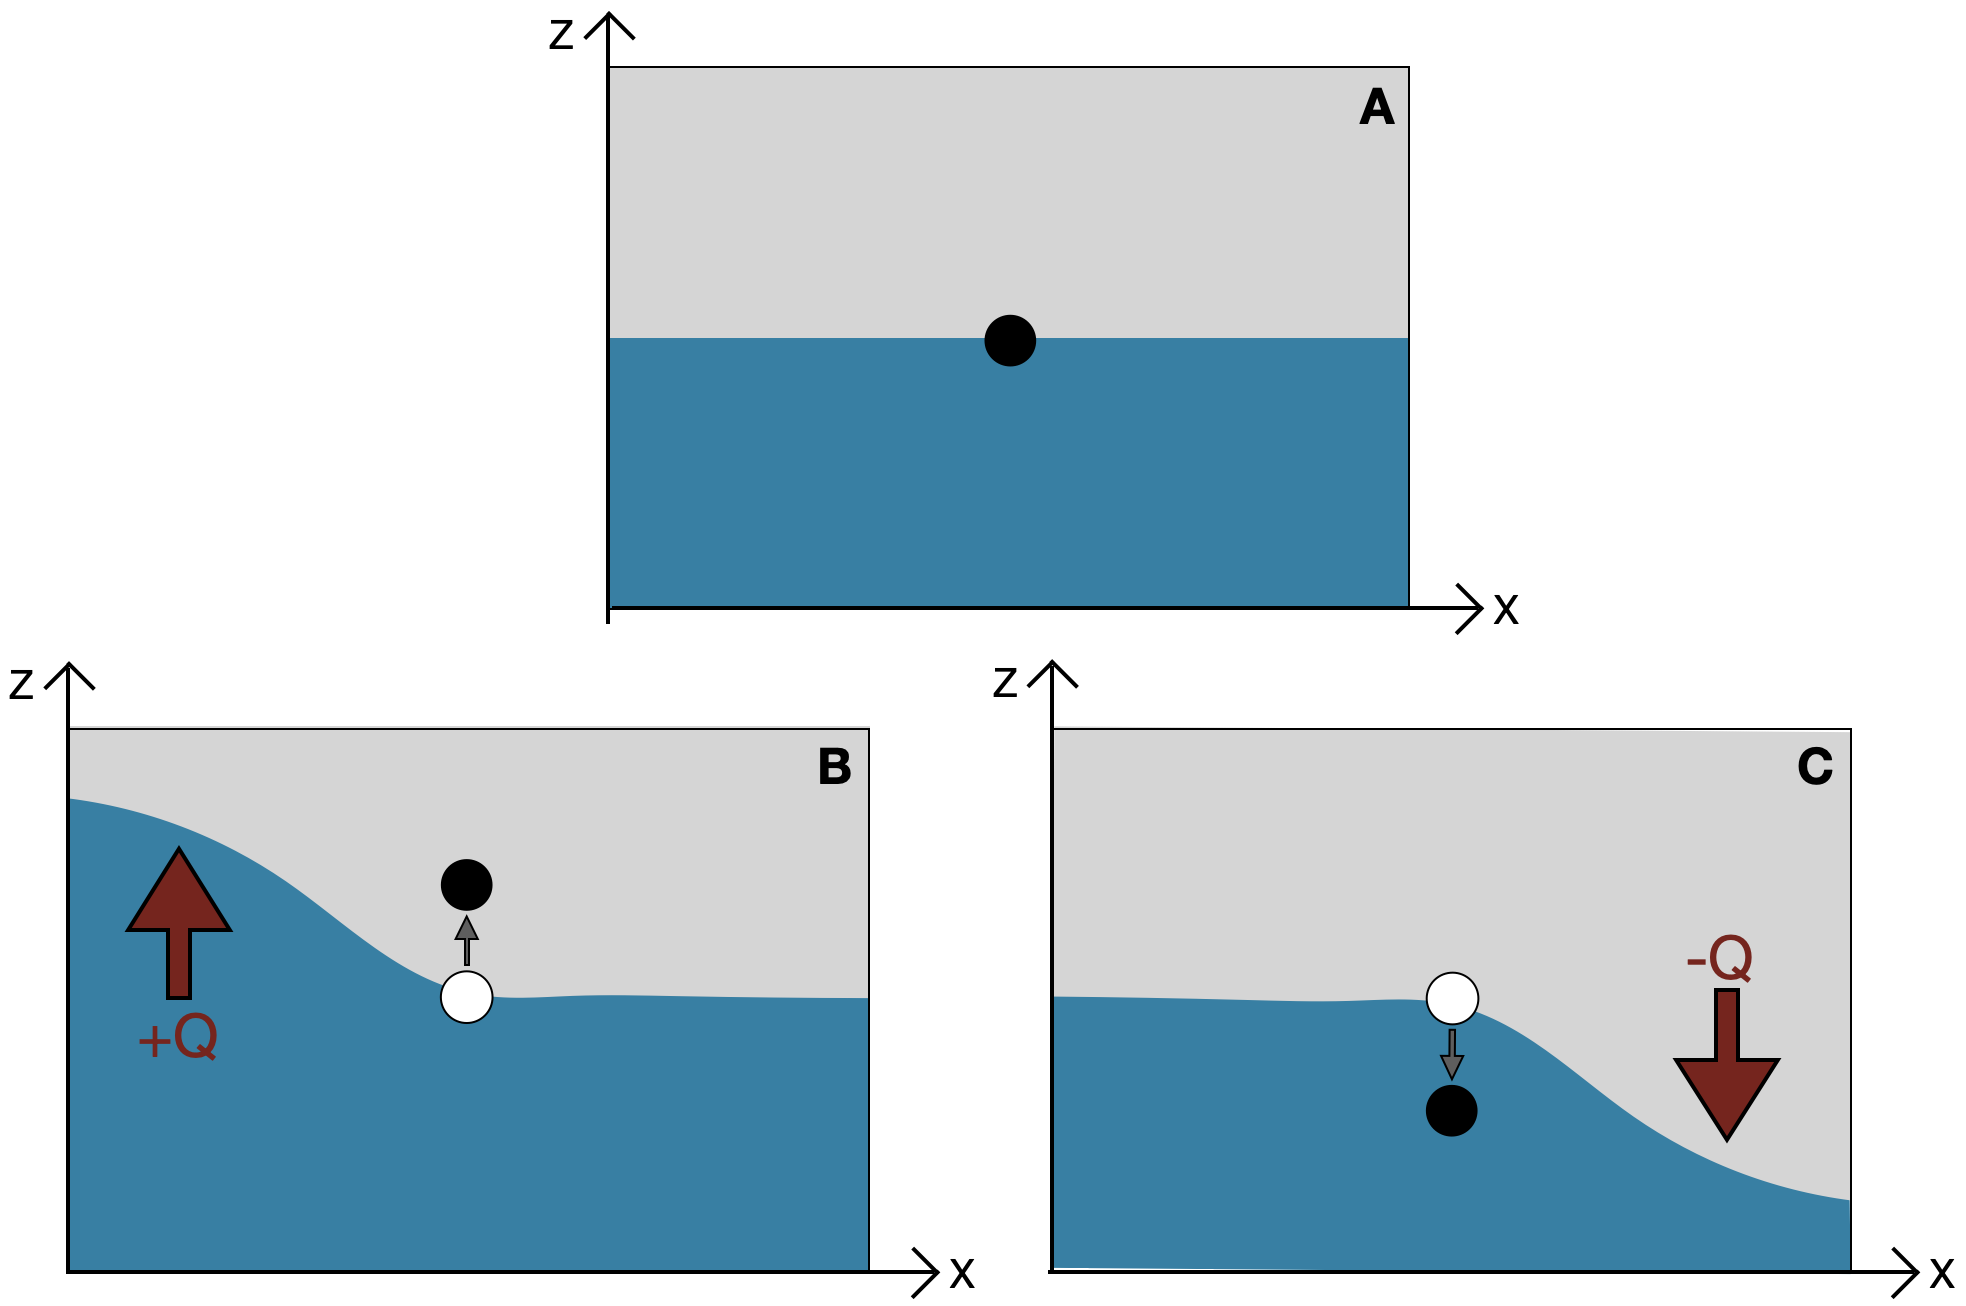
\includegraphics[width=0.7 \columnwidth,angle=0]{fig/energia_potencial.png}
\caption[Effects of Heating and Cooling on Potential Energy]{Mental experiment proposed by \citet{lorenz1955} to illustrate the relationship between total P and K, depicted through a two-layer atmospheric model: (A) Initially horizontally stratified atmosphere. (B) Perturbation caused by localized heating (+Q) leading to vertical upward movements. (C) Similar perturbation caused by cooling (-Q) resulting in vertical downward movements. Black circles represent the atmosphere's center of mass post-perturbation, and white circles indicate the center of mass prior to perturbation.}
\label{energia_potencial}
\end{center}
\end{figure}

The concept of Available Potential Energy (APE) was initially proposed by \citet{margules1903uber}, who was interested in the processes that generate kinetic energy (K) in storms \citep{marquet2017last}. To understand this concept, we can start from the same situation proposed by \citet{lorenz1955}, where differential heating results in ascending movements and a heterogeneous distribution of mass in the atmosphere (Figure \ref{APE}a). In this case, the resulting pressure gradients cause acceleration of the wind field (Figure \ref{APE}b), redistributing the mass in the atmosphere. Assuming this flow is adiabatic, the final result is a horizontally stratified atmosphere (Figure \ref{APE}c). In the first step, both forms of potential energy (total and available) are at their maximum. With the redistribution of mass, there is an increase in K, while the total and available potential energy decreases. In the final stage, P is minimal, yet not zero, while the APE is zero. Thus, APE can be defined as the amount of potential energy available for conversion into K under an adiabatic distribution of mass.

\begin{figure}[h]
\begin{center}
\setcaptionmargin{1cm}
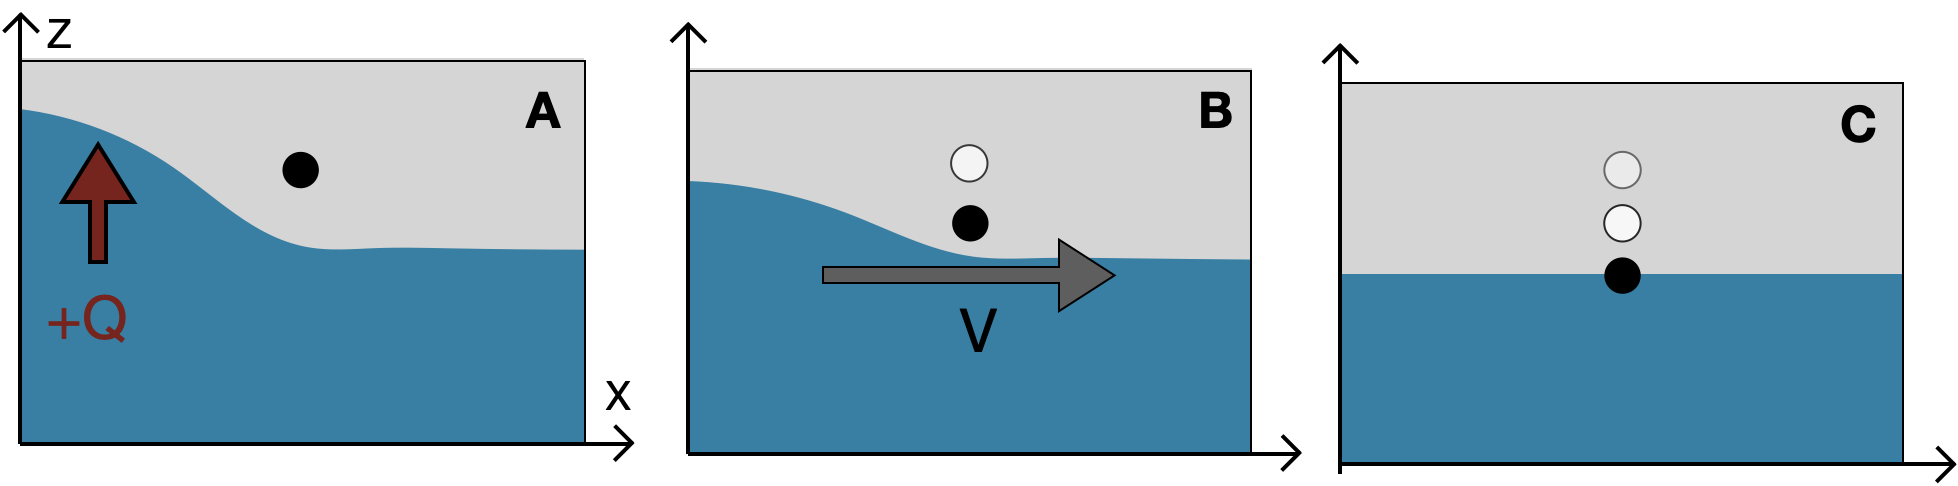
\includegraphics[width=1.0 \columnwidth,angle=0]{fig/APE.png}
\caption[Available Potential Energy]{Depiction of Available Potential Energy (APE) transformations in response to atmospheric heating and cooling. (A) Initial state with differential heating causing heterogeneous mass distribution. (B) Redistribution of mass via wind fields leading to homogenization. (C) Final state of horizontal atmospheric stratification. Black circles indicate the center of mass at each stage, with white circles showing previous positions.}
\label{APE}
\end{center}
\end{figure}

According to \citet{lorenz1955}, APE serves as the primary source of K in the atmosphere, fundamentally driving the general circulation. While APE and K dominantly shape atmospheric dynamics, Lorenz acknowledged that diabatic processes and friction also play critical roles, though these elements were less detailed in his work due to their complex nature and the challenges associated with their quantification. In his theoretical framework, Lorenz treated the atmosphere as a closed system, distinguishing between the zonal and eddy (turbulent) components of APE and K to clarify the energetics involved in atmospheric processes.

This distinction is crucial as it aligns with earlier observations by \citet{starr1953note}, who emphasized the significance of eddies in maintaining atmospheric circulation, particularly their role in transferring K from turbulent to zonal flows. This perspective challenged earlier assumptions and highlighted the necessity of including eddy dynamics in any comprehensive atmospheric circulation theory. Subsequent research by \citet{wiin1963atmospheric} demonstrated the importance of eddies in global heat and momentum transport, illustrating how different wave numbers contribute to these processes. Through these insights, Lorenz's separation of energy components facilitates a deeper understanding of how meteorological systems, such as cyclones, develop and influence broader atmospheric circulation patterns.

The energy cycle can be represented by the following equations, which represent the energy balance for each component of the cycle:

\begin{flalign}
\frac{\partial A_Z}{\partial t} &= -C_Z - C_A + G_Z \\
\frac{\partial A_E}{\partial t} &= -C_E + C_A + G_E \\
\frac{\partial K_Z}{\partial t} &= C_Z - C_K - D_Z \\
\frac{\partial K_E}{\partial t} &= C_E + C_K - D_E 
\end{flalign}

In these equations, available potential energy (APE) is divided into zonal (\(A_Z\)) and eddy (\(A_E\)) components, as is kinetic energy (\(K_Z\) and \(K_E\), respectively). The transformations between these forms of energy are denoted by \(C\), with subscripts \(Z\) and \(E\) for conversions between zonal and eddy forms, and \(A\) and \(K\) indicating conversions between APE and kinetic energy, respectively. Thus, \(C_A\) represents the conversion between \(A_Z\) and \(A_E\), \(C_E\) denotes the conversion from \(A_E\) to \(K_E\), \(C_K\) signifies the transformation from \(K_E\) to \(K_Z\), and \(C_Z\) describes the conversion from \(A_Z\) to \(K_Z\). Generation of APE and dissipation of kinetic energy are indicated by \(G\) and \(D\), with \(G_Z\) and \(G_E\) marking the generation of \(A_Z\) and \(A_E\), and \(D_Z\) and \(D_E\) representing the dissipation of \(K_Z\) and \(K_E\), respectively. Full mathematical formulations for these processes are discussed in Section \ref{math}.

After the seminal work by \citet{lorenz1955} on the global energy cycle, numerous subsequent studies aimed to quantify this cycle, primarily focusing on the Northern Hemisphere due to observational constraints at the time \citep[e.g.]{starr1959further, saltzman1961further, holopainen1964investigation, jensen1961energy, brown1964diagnostic, wiin1959study}. \citet{oort1964estimates} synthesized these results to depict the annual energy cycle of the Northern Hemisphere. He innovatively categorized the energy analysis into distinct domains: the spatial domain, where variables are analyzed based on spatial averages, aiding in the understanding of large-scale zonal patterns such as jet streams and westerlies; the temporal domain, focusing on averages and deviations over time, which facilitates insights into long-term trends and transient disturbances; and the mixed space-time domain, which offers an integrated perspective on how average states and disturbances, both transient and stationary, interact and are sustained. Oort noted that while there was considerable focus on spatial domain analyses, studies addressing the mixed domain were scarce, and those considering the temporal domain were virtually absent.

From these estimates, \citet{oort1964estimates} presented a diagram that visually encapsulates the energy cycle (Figure \ref{LEC_simples}). This diagram illustrates the generation, conversion, and dissipation of different energy forms, providing a dynamic overview in a graphical format. Notably, the diagram allows for straightforward comparisons of diverse study results. It is important to mention, as \citet{oort1964estimates} did, that friction terms are typically calculated as residuals due to the challenges in direct computation, balancing the zonal and turbulent terms of kinetic energy.

\begin{figure}[h]
\begin{center}
\setcaptionmargin{1cm}
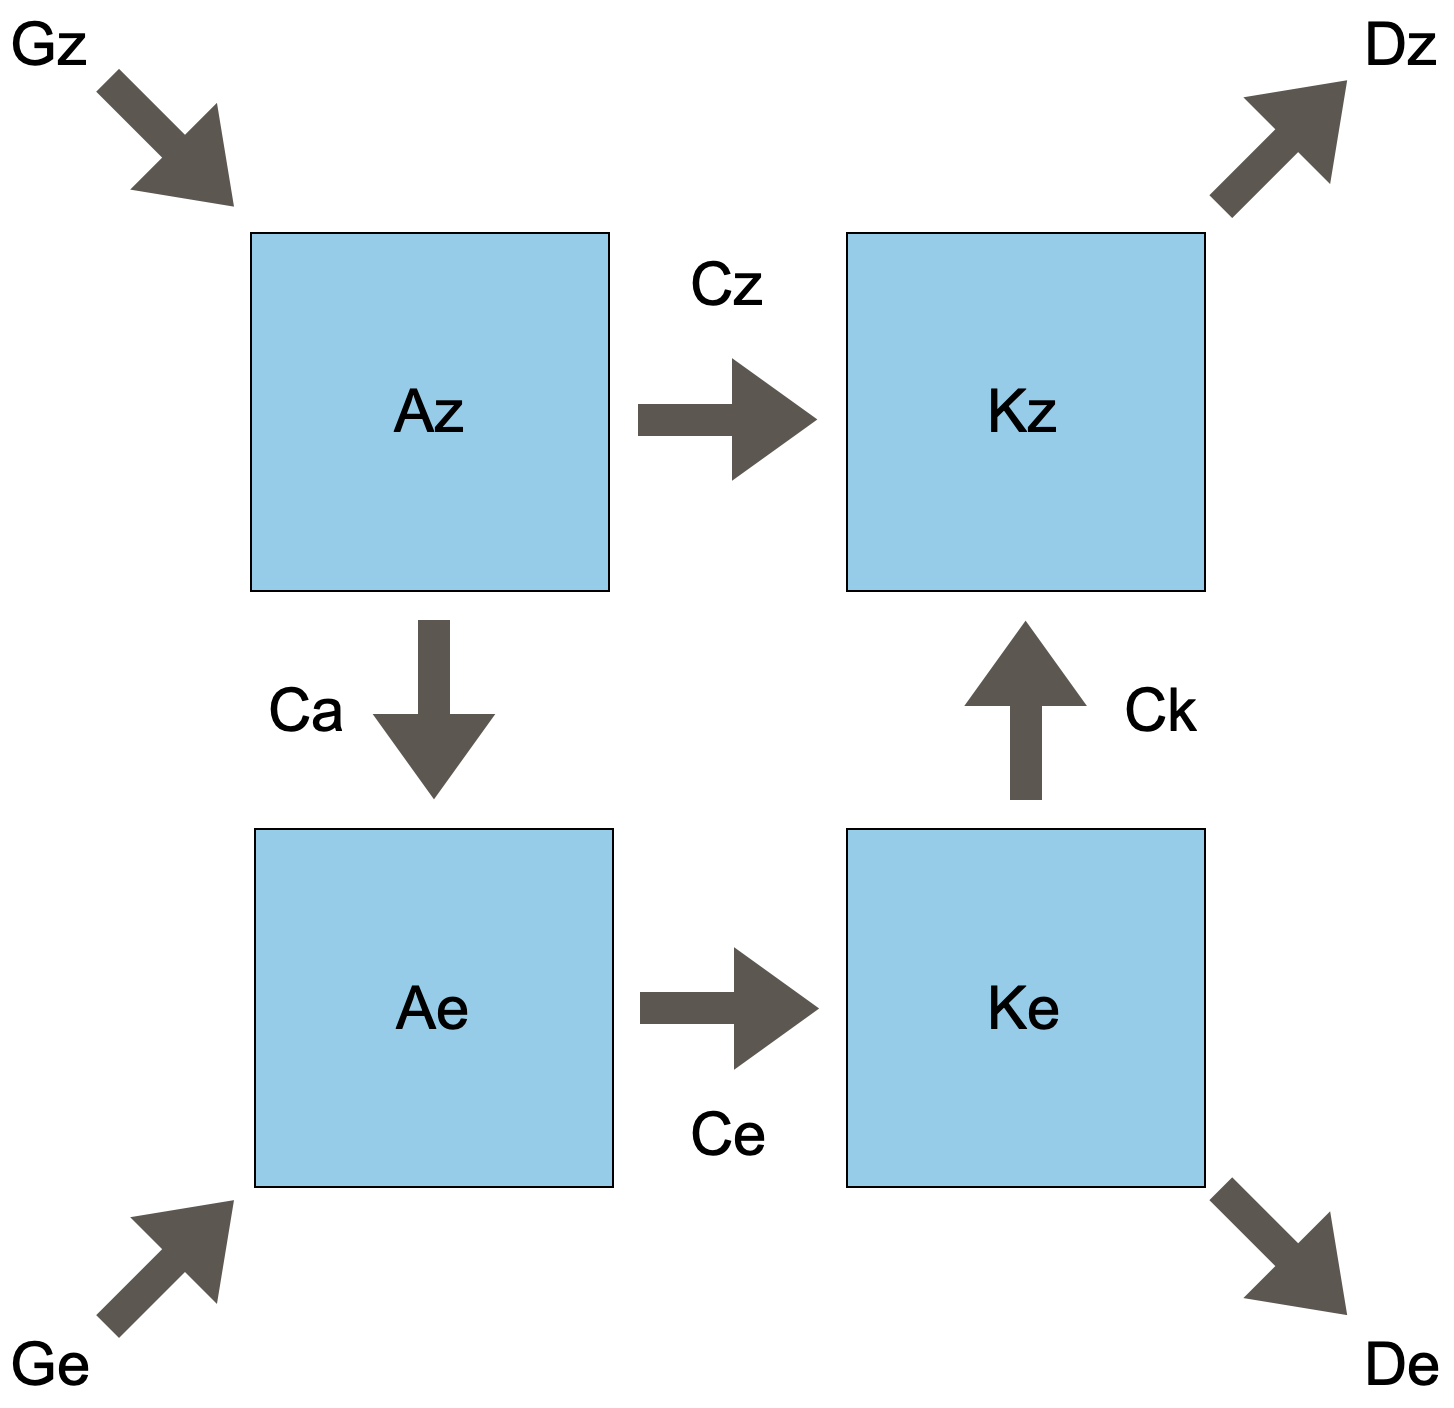
\includegraphics[width=0.5 \columnwidth,angle=0]{fig/LEC_simples.png}
\caption[Energy Cycle - Lorenz]{Representation of the energy cycle as formulated by \citet{lorenz1955} and schematized by \citet{oort1964estimates}. This diagram displays the interplay among the four forms of energy (zonal and turbulent terms of K and APE), illustrating their conversions, generation, and dissipation.}
\label{LEC_simples}
\end{center}
\end{figure}

As previously mentioned, the formulation proposed by \citet{lorenz1955} estimates the energetics of the atmosphere assuming a closed system, that is, without energy exchanges at the boundaries. The first study to consider energetics for an open system was by \citet{reed1963spectral}, which analyzed a sudden stratospheric warming event in the Northern Hemisphere. This study treated the stratosphere as an open system, permitting energy exchanges with other atmospheric layers, such as the troposphere. Building on this, \citet{muench1965dynamics}, who was interested in stratospheric dynamics, refined \citet{lorenz1955}'s theory and proposed a new representation of the energy cycle.

Muench's model adds boundary flow terms (\( BA_Z \), \( BA_E \), \( BK_Z \), and \( BK_E \)) to the original Lorenz equations, representing respectively the zonal and eddy flows of APE and K across the system boundaries (Figure \ref{LEC_Muench}). The updated energy balance equations are:

\begin{flalign}
\frac{\partial A_Z}{\partial t} &= BA_Z - C_Z - C_A + G_Z \\
\frac{\partial A_E}{\partial t} &= BA_E - C_E + C_A + G_E \\
\frac{\partial K_Z}{\partial t} &= BK_Z + C_Z - C_K + B\Phi_Z - D_Z \\
\frac{\partial K_E}{\partial t} &= BK_E + C_E + C_K + B\Phi_E - D_E 
\end{flalign}

Where \(BA_Z\), \(BA_E\), \(BK_Z\), and \(BK_E\) represent, respectively, the flows of zonal and eddy APE and K across the boundaries. The terms \(B\Phi_Z\) and \(B\Phi_E\) are represented together with the terms \(C_Z\) and \(C_E\), respectively, because both arise from the same process of deriving the balances of \(K_Z\) and \(K_E\). \citet{muench1965dynamics} recognizes the difficulty in interpreting the terms \(B\Phi_Z\) and \(B\Phi_E\), indicating that they are related to the flow of kinetic energy towards lower altitudes, representing the emergence of kinetic energy at the boundaries of the computational domain.

\begin{figure}[h]
\begin{center}
\setcaptionmargin{1cm}
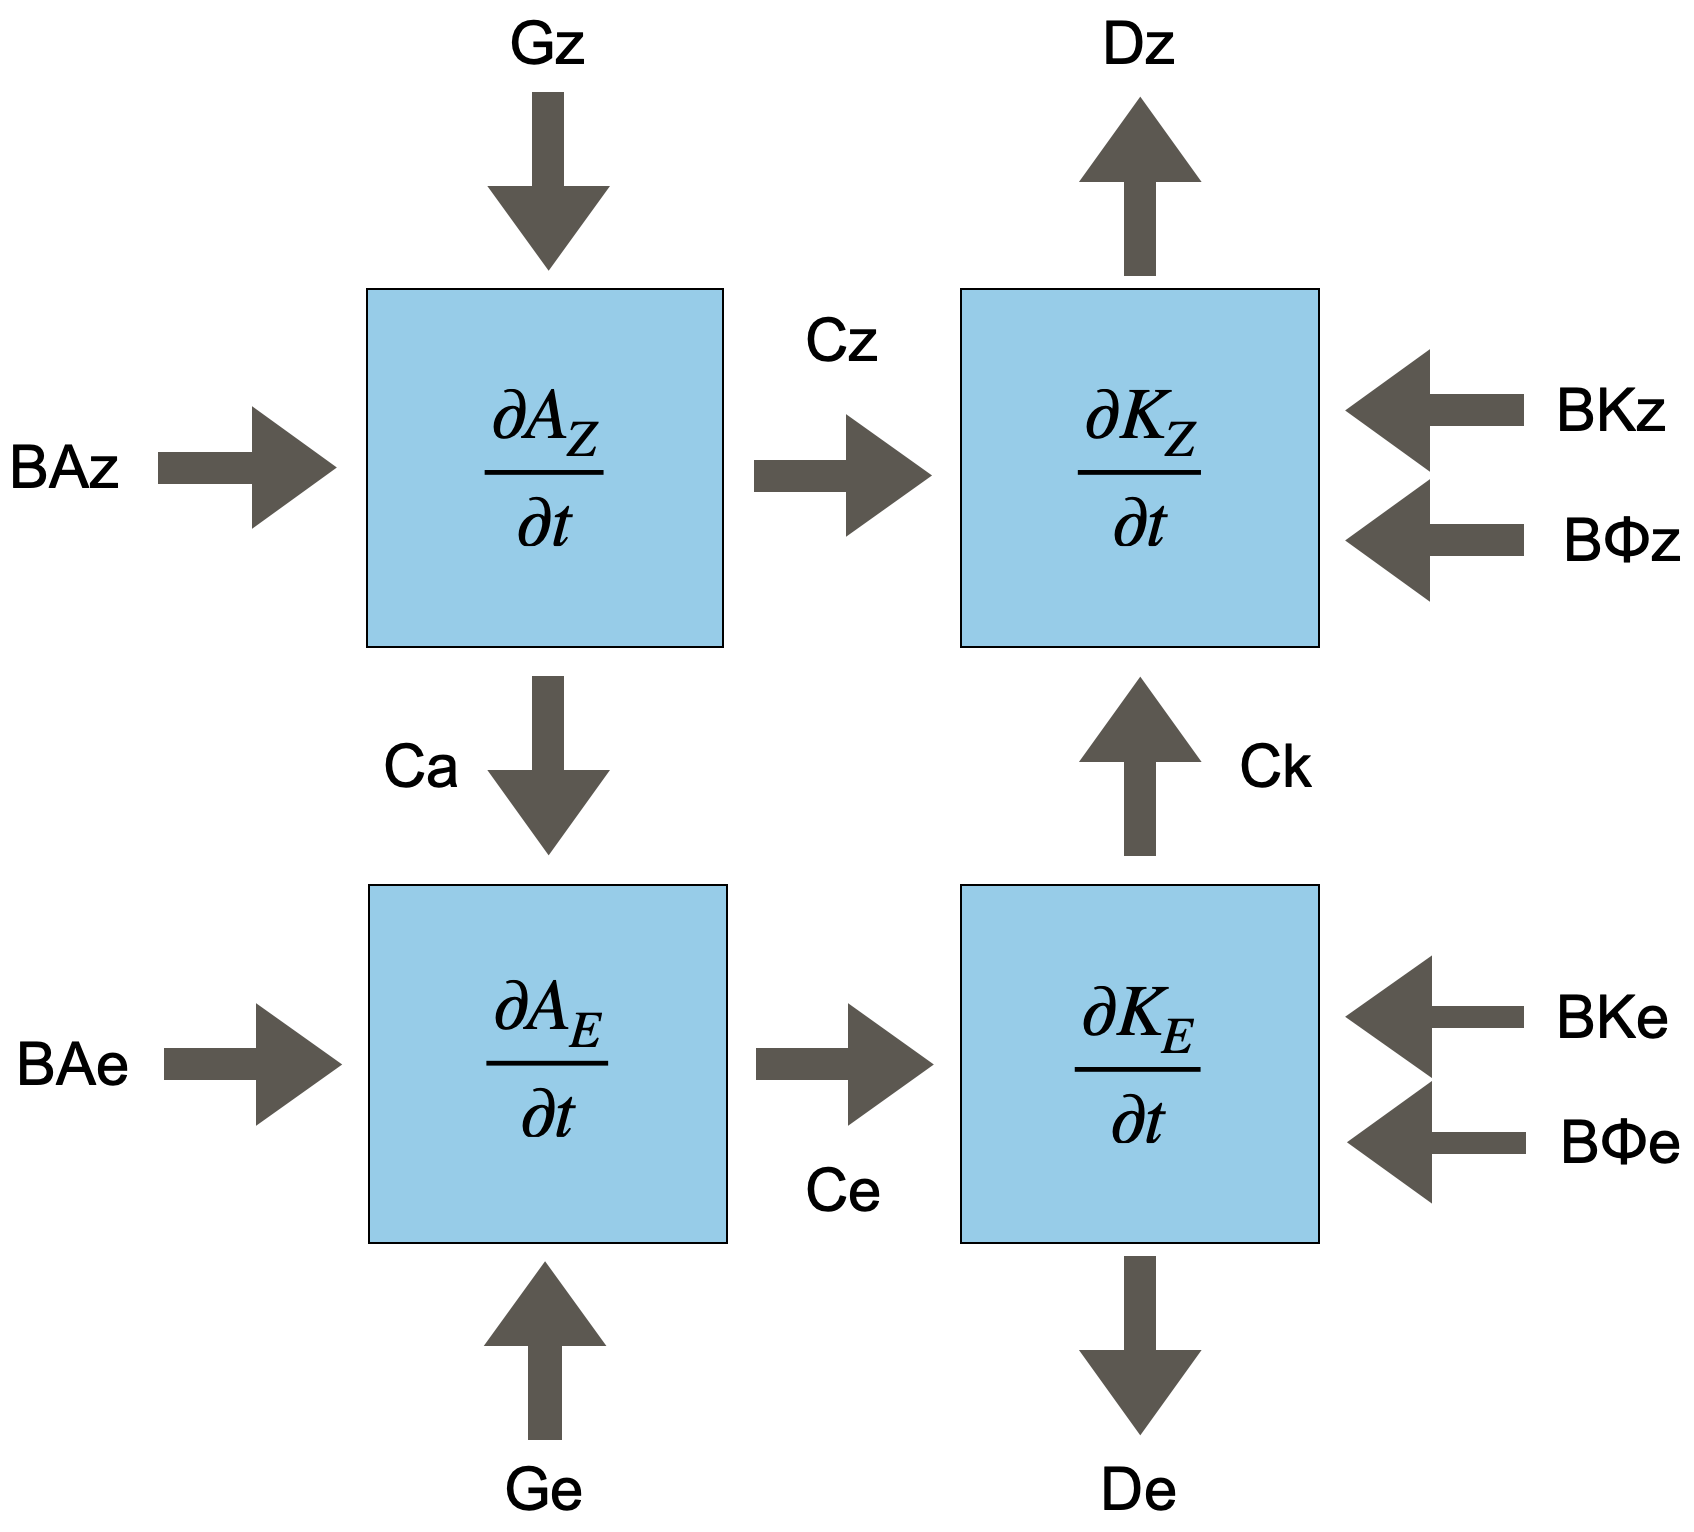
\includegraphics[width=0.5 \columnwidth,angle=0]{fig/LEC_Muench.png}
\caption[Energy Cycle - Muench]{Energy cycle as formulated by \citet{lorenz1955} and updated by \citet{muench1965dynamics}. This diagram includes additional terms representing energy flows across boundaries, illustrating both the local derivatives of the zonal and eddy partitions of APE and K and the interactions at the system edges.}
\label{LEC_Muench}
\end{center}
\end{figure}

Although Muench's model considers boundary flows, his domain was partially open, extending up to the polar regions and encompassing the entire Northern Hemisphere longitudinally, with the only boundary at the southern part of the domain at 30$^\circ$N. The notion of a fully regional energy cycle was later approached by \citet{smith1969contribution}, who aimed to assess the contribution of a limited region to global energetics. Smith clarified that while his work presented a framework for regional analysis, an exact computation of local energetics was outside its scope, and his model did not differentiate between zonal and eddy components of APE and K.

Parallel to the work by \citet{smith1969contribution}, \citet{johnson1970available}, following the theoretical framework proposed by \citet{dutton1967theory}, introduced a semi-Lagrangian framework for analyzing the energy cycle of limited areas. In this formulation, the delineated area for performing energetic calculations moves with the meteorological system of interest, spanning $N$ fixed regions that shift in space. This analysis highlights that global Available Potential Energy (APE) is the aggregate of all possible open atmospheric regions, plus a term representing the thermodynamic contrast among these regions. It's crucial to note that \citet{smith1969contribution} and \citet{dutton1967theory} argued that the APE of a limited region should be viewed as its contribution to the global energetics rather than a standalone quantity. This perspective stems from the interconnected nature of the atmosphere, where local and global energetics are mutually influential. 

\citet{dutton1967theory} also critiqued \citet{lorenz1955}'s formulation, pointing out its underestimation of APE, particularly during the winter months. The alternative set of equations introduced by \citet{johnson1970available}, which utilizes isentropic coordinates, however, included simplifications that were seen as limitations by \citet{vincent1973some}, such as neglecting the impact of diabatic heating, rendering it impractical for diagnostic applications. Following this rationale, \citet{vincent1973some} developed a system of equations in isobaric coordinates that account for the balances of APE and Kinetic Energy (K) in an open atmospheric system from a semi-Lagrangian perspective. 

This formulation partitions APE into the reference state APE of the region and two components representing barotropic and baroclinic contributions to the APE of the delineated area. The balance equations for APE now included terms for boundary movement in the semi-Lagrangian frame and the advection of air masses with varying properties across these boundaries. This formulation was first applied by \citet{edmon1979large} in an energy cycle analysis of Hurricane Carmen (1974). Building on this, \citet{brennan1980zonal} adapted Vincent's approach to incorporate zonal and eddy components of APE and K, marking the first instance of such a detailed and realistic equation set being applied to a limited are within the troposphere. However, \citet{brennan1980zonal} utilized a traditional Eulerian approach for their energy analysis.

Furthermore, \citet{brennan1980zonal} reinterpreted the boundary terms \(B\Phi_Z\) and \(B\Phi_E\) as the work done by zonal and meridional wind components against atmospheric pressure at the computational domain boundaries. However, they noted that these terms, as calculated, were unrealistically large due to minor errors in the geopotential height field, which could escalate in major errors and significantly skew the results. Consequently, these terms were combined with the dissipation terms (\(D_Z\) and \(D_E\)) and treated as residuals in the balance equations for \(K_Z\) and \(K_E\), resulting in new terms \(RK_Z\) and \(RK_E\). This approach and the updated energy cycle are depicted in Figure \ref{LEC_Brennan}.


\begin{figure}[h]
\begin{center}
\setcaptionmargin{1cm}
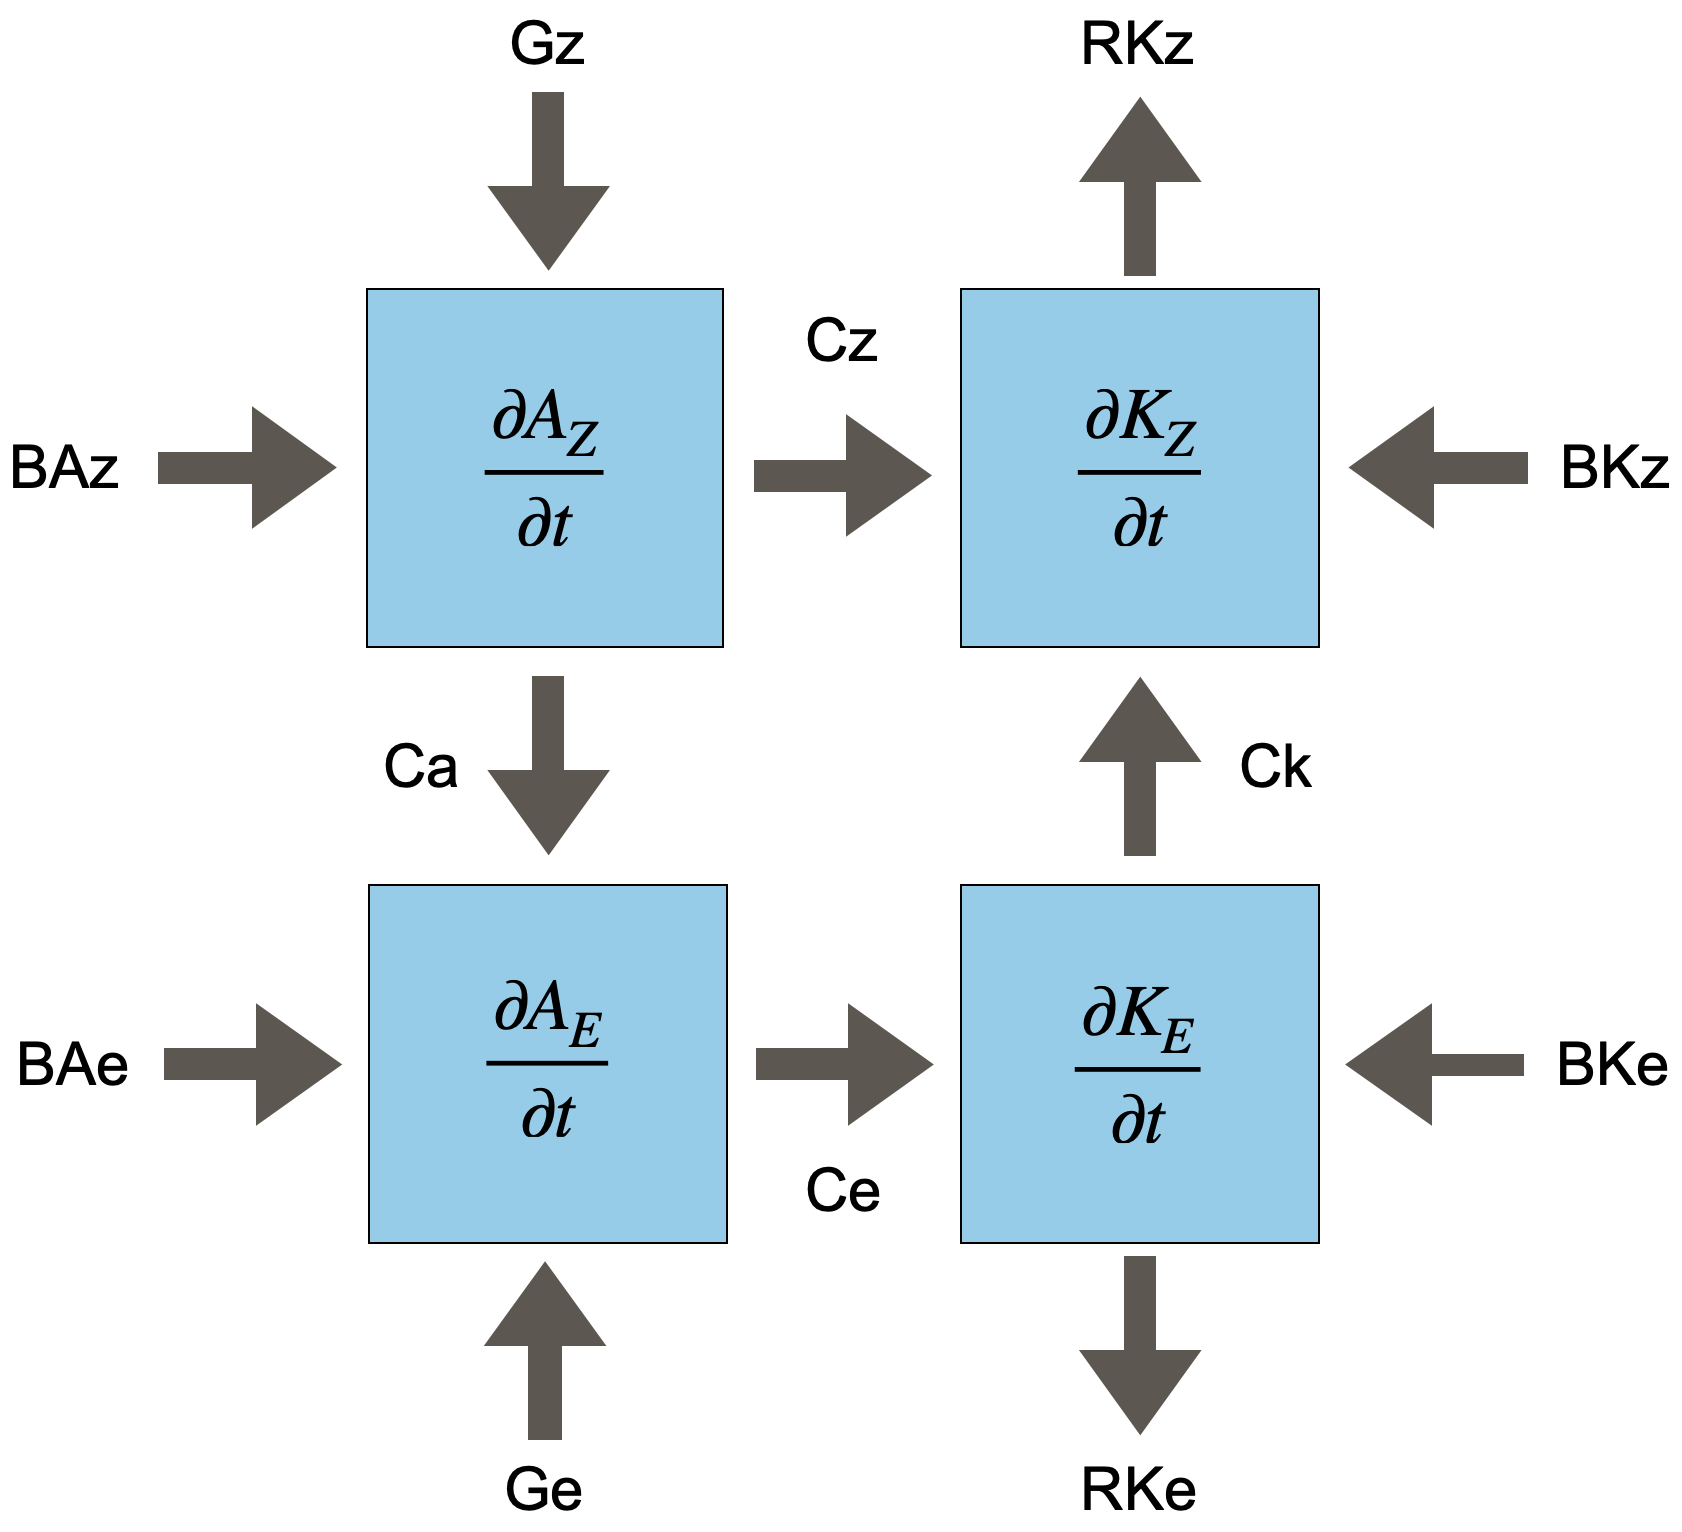
\includegraphics[width=0.5 \columnwidth,angle=0]{fig/LEC_Brennan.png}
\caption[Energy Cycle - Brennan]{Updated energy cycle as reformulated by \citet{brennan1980zonal}. This diagram includes the integrated terms for boundary energy flows (\(B\Phi_Z\) and \(B\Phi_E\)) merged with dissipation processes (\(D_Z\) and \(D_E\)), represented as residual terms \(RK_Z\) and \(RK_E\).}
\label{LEC_Brennan}
\end{center}
\end{figure}

The modified energy balance equations are as follows:

\begin{flalign}\label{balanco_Brennan}
\frac{\partial A_Z}{\partial t} &= -C_A - C_Z + G_Z + BA_Z \\
\frac{\partial A_E}{\partial t} &= C_A - C_E + G_E + BA_E  \\
\frac{\partial K_Z}{\partial t} &= C_K + C_Z + BK_Z + RK_Z \\
\frac{\partial K_E}{\partial t} &= - C_K + C_E + BK_E  + RK_E 
\end{flalign}

And the residual terms are defined as:

\begin{flalign}\label{residuo_K}
RK_Z &= B\Phi_Z + D_Z \\
RK_E &= B\Phi_E + D_E 
\end{flalign}


\citet{robertson1983impact} adapted the formulation presented by \citet{brennan1980zonal} for limited area domains, particularly revising the term $A_E$. Building upon the framework of APE for limited domains outlined by \citet{smith1977time}, Robertson integrates the first law of thermodynamics into the Eulerian derivatives of the APE and $A_Z$ formulations. This results in a significantly different balance equation for $A_E$, introducing a novel term associated with variations in the reference pressure field, which alters the computation of the conversion term $C_A$. This approach was driven by the goal of evaluating, through numerical modeling, the influence of moist processes on the energetics of extratropical cyclones. However, the adaptation necessitated computations over isentropic coordinates, introducing complexities in the numerical implementation.

In an effort to analyze the energetics of cyclogenesis in the Gulf of Genoa within the Mediterranean Sea, \citet{michaelides1987limited} advanced the energy cycle formulation further. Echoing concerns from \citet{brennan1980zonal} regarding unrealistic results for the terms $B\Phi_{Z}$ and $B\Phi_{E}$, Michaelides introduced additional residual terms $RK_Z$ and $RK_E$, and a correction factor ($\epsilon$) to account for numerical errors in the estimation of these terms, as shown in the equations and Figure \ref{LEC_Michaelides}. The modified set of equations is as follows:

\begin{flalign}\label{balanco_Michaelides}
\frac{\partial A_Z}{\partial t} &= C_K - C_A + BA_Z + \Delta G_Z \\
\frac{\partial A_E}{\partial t} &= C_A - C_E + BA_E + \Delta G_E  \\
\frac{\partial K_Z}{\partial t} &= C_K - C_Z + BK_Z - \Delta R_Z \\
\frac{\partial K_E}{\partial t} &= C_E - C_K + BK_E - \Delta R_E 
\end{flalign}

Where the residual terms are defined as:

\begin{flalign}\label{residuo_Michaelides}
\Delta R_Z &= B\Phi_Z - D_Z + \epsilon_{KZ} \\
\Delta R_E &= B\Phi_E - D_E + \epsilon_{KE} \\
\Delta G_Z &= G_Z + \epsilon_{GZ} \\
\Delta G_E &= G_E + \epsilon_{GE}
\end{flalign}

\begin{figure}[h]
\begin{center}
\setcaptionmargin{1cm}
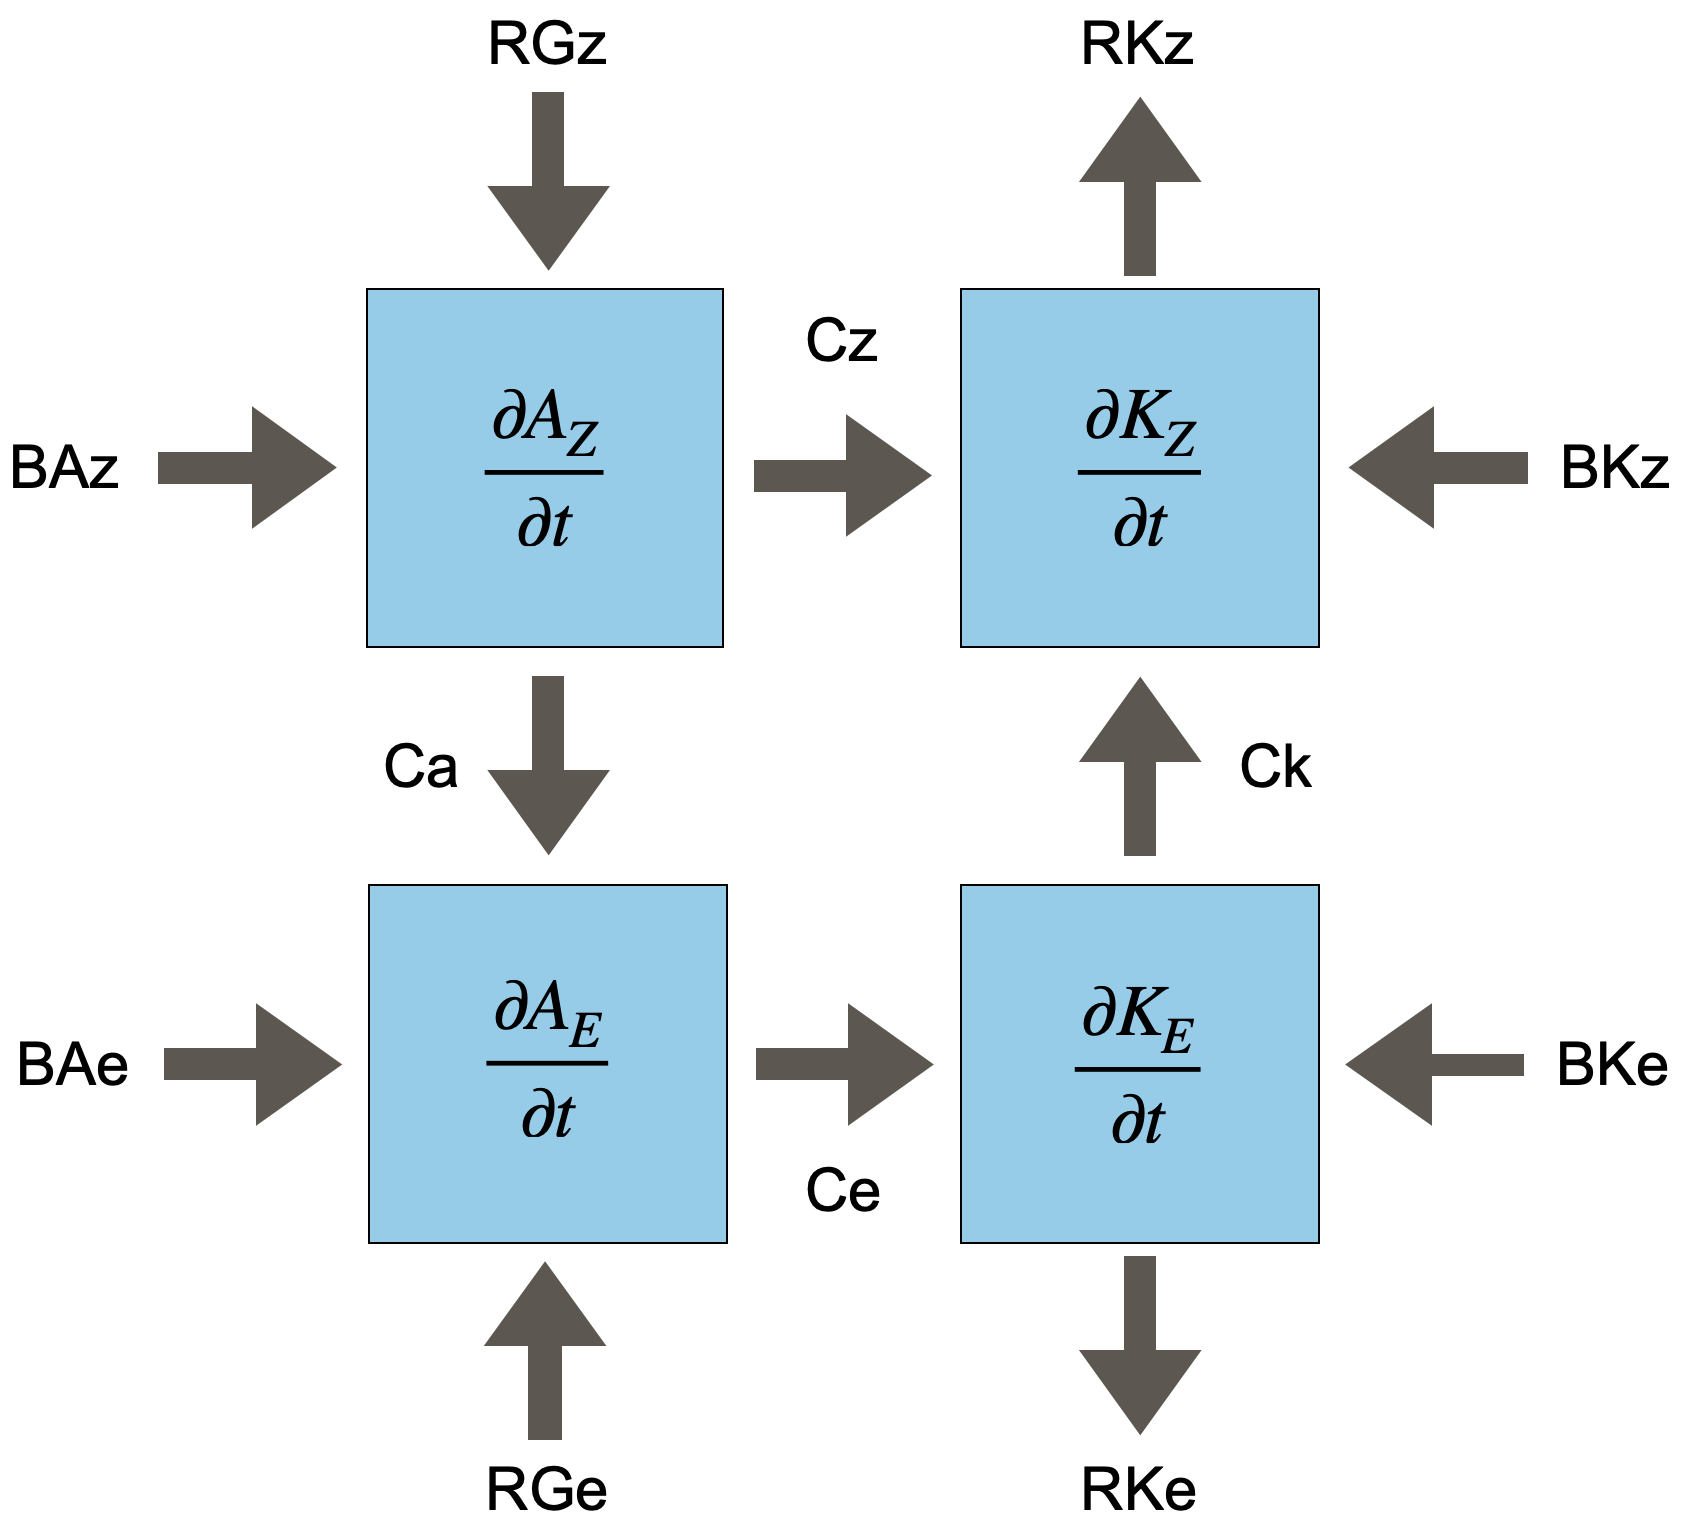
\includegraphics[width=0.5 \columnwidth,angle=0]{fig/LEC_Michaelides.png}
\caption[Energy Cycle - Michaelides]{Refined depiction of the energy cycle incorporating modifications by \citet{michaelides1987limited}. This representation includes error correction terms within the residual balances, addressing previous challenges with the quantification of boundary terms and dissipation factors.} 
\label{LEC_Michaelides}
\end{center}
\end{figure}

In \citet{michaelides1999quasi}, the author extends the energetic formulations presented in \citet{michaelides1987limited}, exploring calculations for limited areas using both Eulerian and semi-Lagrangian reference frames. This study evaluates the energy cycle during a cyclogenesis event in the Mediterranean from these two perspectives, providing a nuanced discussion on the methodological implications of each. It highlights that the Eulerian approach is commonly preferred for energy analysis in limited atmospheric areas. This method necessitates defining a sufficiently large spatial domain to encapsulate all developmental stages of the system, including its movement and size changes. However, this approach has interpretative limitations; a broad spatial domain may inadvertently include adjacent synoptic circulations, thus diluting the specific energetics of the primary system under study.

Figure \ref{fixed_framework_issues} illustrates this issue with a scenario akin to cyclogenesis in the coastal region of Southeast Brazil \citep[e.g.,]{reboita2010south, gramcianinov2019properties}. Here, the computational domain must encompass both the initial coastal genesis area and the subsequent oceanic trajectory of the cyclone. As the cyclone progresses to the ocean in its later stages, mesoscale circulations near the coast, such as updrafts due to surface heating and convection from sea breeze interactions with local topography, emerge. These processes can significantly alter the computed values of APE and K within the domain, affecting the energy conversion, boundary, dissipation, and generation terms, thereby complicating the interpretation of the cyclone's energy dynamics.

\begin{figure}[h]
\begin{center}
\setcaptionmargin{1cm}
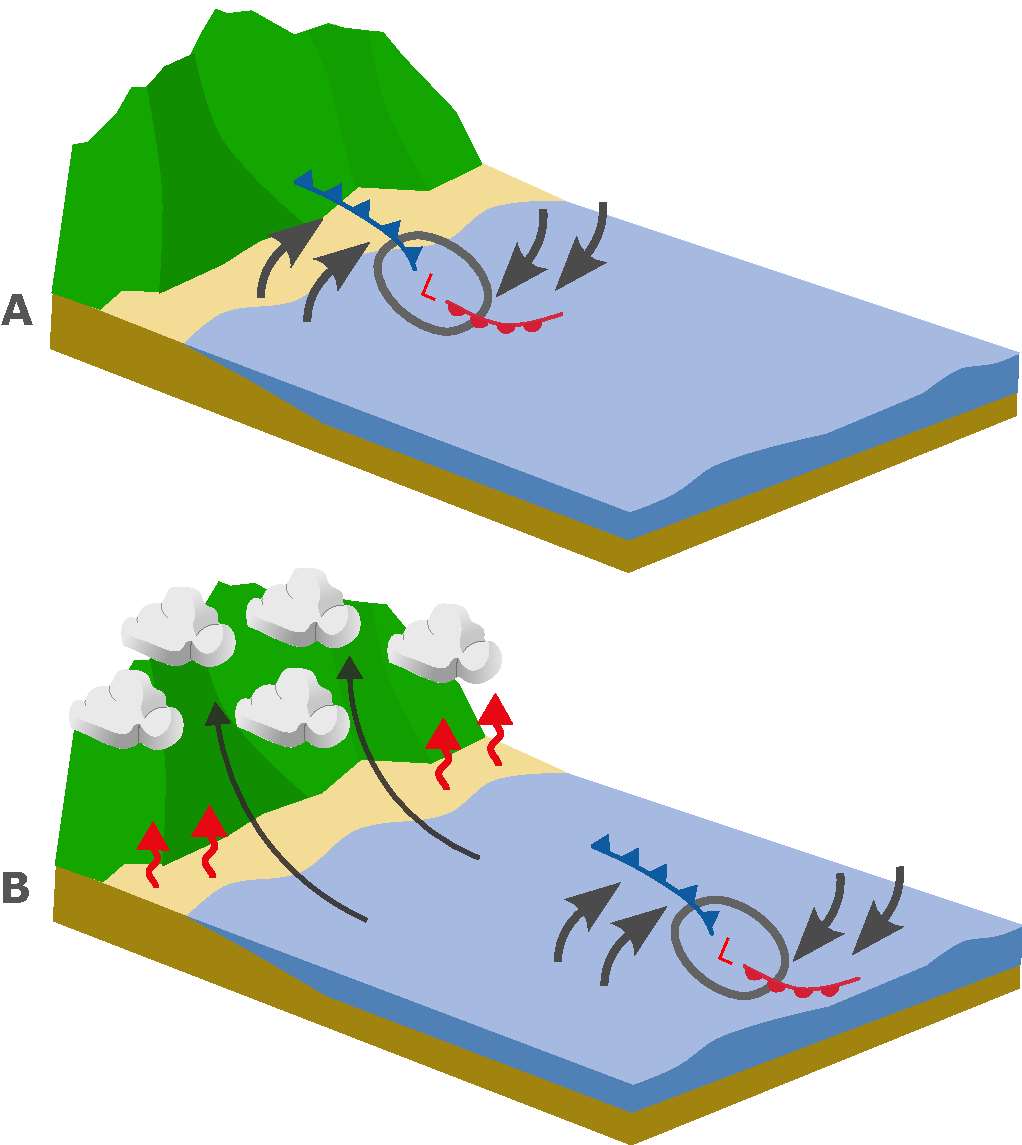
\includegraphics[width=0.5 \columnwidth,angle=0]{fig/limited_area_energetics_example.pdf}
\caption[Eulerian LEC - Issues]{Illustration of challenges in using an Eulerian reference frame for energy cycle analysis. A) A cyclone forming near the continent, where the newly developed cyclonic system is the main meteorological feature inside the domain. B) The system is in its later oceanic phase, while meso-scale circulations develop in the coastal region, such sea-breeze and, consequently, orographic ascent over the mountain range near the coast.}
\label{fixed_framework_issues}
\end{center}
\end{figure}


Despite the inherent limitations associated with the Eulerian approach, \citet{michaelides1999quasi} discusses the methodological challenges of employing a purely Lagrangian framework to study extratropical cyclones. Such a study would require tracking the system in a three-dimensional space, isolated from external influences, using specific conservative variables for the encapsulated air masses. This is complicated by the diverse origins of the air masses involved in extratropical cyclones, which include both polar and tropical sources, affecting their conservative properties. Additionally, the system must be isolated from any spurious external circulations.

Consequently, \citet{michaelides1999quasi} advocates for a quasi-Lagrangian approach as a practical solution that minimizes the impact of neighboring circulations on the system's energy dynamics. This approach, similar to that proposed by \citet{vincent1973some}, utilizes multiple fixed domains at different temporal intervals to effectively track the cyclonic system. However, unlike \citet{vincent1973some}, \citet{michaelides1999quasi}'s formulation does not include terms for the displacement of computational domain boundaries. The author conducts a comparative analysis between the Eulerian and quasi-Lagrangian methods, revealing that they can yield significantly different results depending on the specific energetic terms analyzed. This highlights the complications in using the Eulerian method for comparative studies, as it can incorporate the energetic contributions of adjacent systems. \citet{michaelides1999quasi} concludes that the semi-Lagrangian method offers a more robust framework for analyzing the energetics of cyclonic systems.

Nevertheless, critiques of the quasi-Lagrangian approach exist \citep[e.g.]{dias2011energy}. One major criticism is that this method does not allow for the local time derivatives of energy terms due to the absence of a fixed computational volume, which impedes a complete closure of the energy balance — a limitation acknowledged by \citet{michaelides1999quasi}. Additionally, there is debate over whether changes in the energetics through the cyclone lifecycle can be attributed to the system's dynamics or to the fact that the tracking box may capture varying environmental conditions. However, these perceived limitations can be addressed by understanding that the distinct boxes used at each time-step through the cyclone's lifecycle are effectively "snapshots" of its dynamics. Consider the following thought experiment: we compute the LEC using both quasi-Lagrangian and Eulerian frameworks. The quasi-Lagrangian experiment tracks the trajectory of an extratropical cyclone, using a distinct \(15^\circ \times 15^\circ\) domain for each hourly time step. Meanwhile, the Eulerian experiment employs a fixed \(15^\circ \times 15^\circ\) domain in a specific location, which will coincide with the cyclone's trajectory at a given time step, thereby exactly matching the domain used in the quasi-Lagrangian framework. As demonstrated in Section \ref{math}, the equations used in LEC computation do not have temporal dependencies; therefore, for this specific time where the domains of both frameworks overlap, the results will be identical. At this time step, the quasi-Lagrangian domain likely contains only the cyclonic system, thus the computed energetics are indisputably linked to its development at that moment — or, using \citet{smith1969contribution}'s interpretation: the system's contribution to global energetics. Following this reasoning, it is logical to assume that each domain in the quasi-Lagrangian approach represents the cyclone energetics for each specific time step, effectively providing snapshots of the energetics.

\begin{figure}[h]
\centering
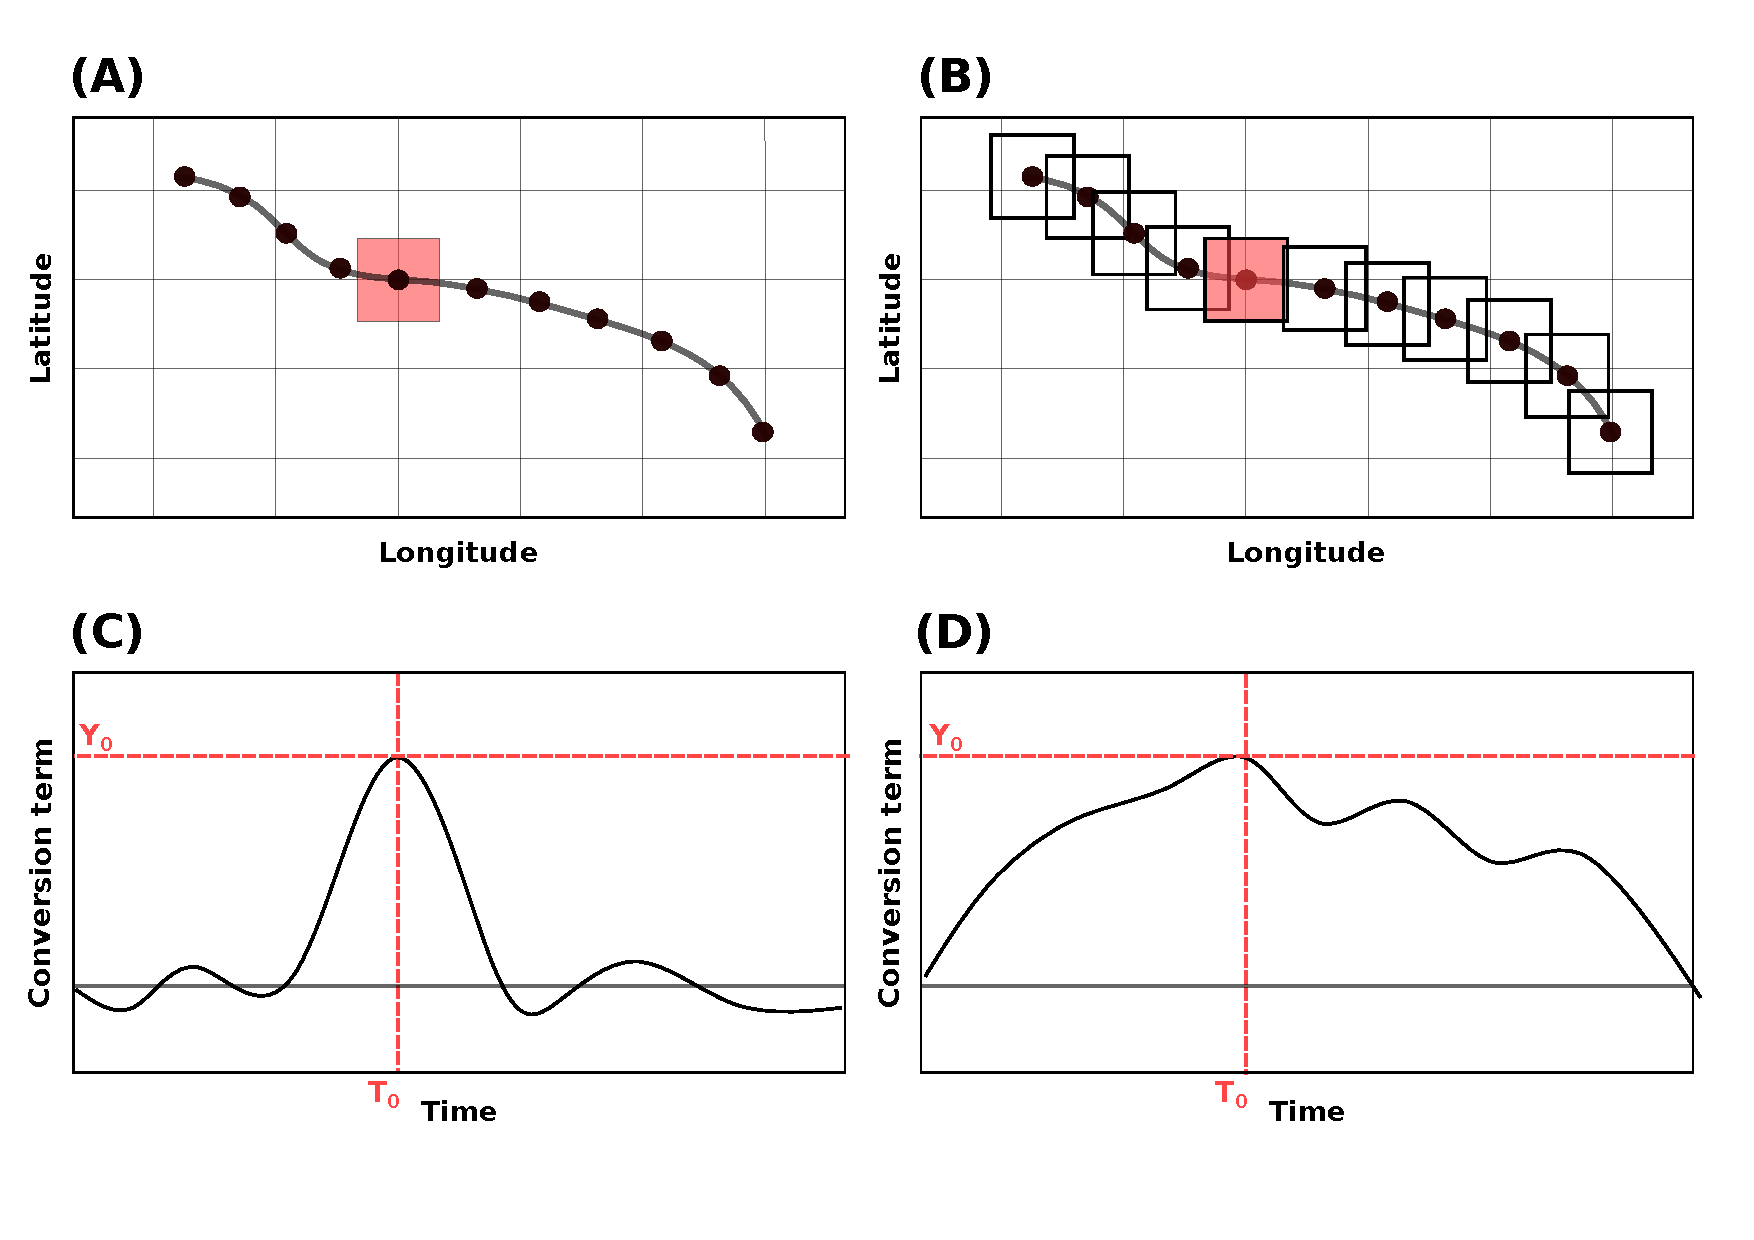
\includegraphics[width=\linewidth]{fig/LEC_argument.pdf}
\caption[LEC - discussion]{Illustration of the quasi-Lagrangian and Eulerian frameworks employed in the LEC computation for analyzing cyclonic energetics. Panel (A) shows the Eulerian approach with a fixed \(15^\circ \times 15^\circ\) domain, overlapping with the cyclone's trajectory at a specific time step ($T_0$). Panel (B) depicts the quasi-Lagrangian approach, tracking a \(15^\circ \times 15^\circ\) domain that moves with the cyclone, providing hourly snapshots. The highlighted domain in Panel (B) indicates the domain at $T_0$ that overlaps with the Eulerian domain from Panel (A). Panels (C) and (D) display a hypothetical conversion term used solely for demonstrating that both frameworks yield identical results ($Y_0$) when the domains coincide. This alignment supports the argument that each quasi-Lagrangian domain snapshot accurately reflects the system's energetics at each respective time step.}
\label{fig:lec_argument}
\end{figure}

Several methodologies have been developed to refine diagnostic equations for atmospheric energetics, each offering unique advancements. The approach introduced by \citet{plumb1983new} critiques traditional energy formulations for wave propagation and employs transformed Eulerian-mean equations to enhance the physical accuracy of eddy-mean flow interactions. Similarly, \citet{marquet1991concept}'s redefinition of exergy and available enthalpy provides a more complete analysis of atmospheric dynamics, accommodating factors such as static instabilities and topographical variations often oversimplified in previous models. The local APE density framework proposed by \citet{novak2018local}, on the other hand, introduces a positive-definite local form of potential energy, akin to kinetic energy, which can be transported, converted, and dissipated locally. Unlike the global and volume-integrated nature of Lorenz’s APE, this local APE density theory adapts potential energy calculations to specific atmospheric conditions, enhancing diagnostic precision in regional climate studies. However, these methods significantly complicate the mathematical formulations, requiring increased computational resources and extending computation times, which pose substantial limitations, especially for operational purposes. Additionally, each of these frameworks introduces new challenges in the physical interpretation of the terms.

The present work adopts the formulation presented by \citet{michaelides1999quasi}, which offers a balance between computational feasibility and physical accuracy. This framework provides results that serve as a useful diagnostic tool, facilitating an understanding of the dynamical mechanisms involved in cyclone development without requiring extensive computational resources. While the primary goal of this thesis is scientific, there is significant interest in developing an operational tool for diagnosing the energy cycle of cyclones that can be made available to the scientific community. This tool is envisioned to function similarly to the Hart phase diagrams, which are accessible online (\href{https://moe.met.fsu.edu/cyclonephase/ecmwf/fcst/index.html}{https://moe.met.fsu.edu/cyclonephase/ecmwf/fcst/index.html}) and widely used for real-time cyclone analysis. The complete mathematical formulation and physical interpretation of each term in the Lorenz Energy Cycle (LEC) are detailed in Section \ref{math}. Additionally, Section \ref{metodos_calculo_lec} describes the computational methods used to calculate the LEC.


\subsection{Lorenz Energy Cycle: Mathematical expressions and physical interpretation}\label{math}

This section provides a detailed description of the symbols and expressions used for the calculation of the Lorenz Energy Cycle (LEC), adopting the notation from \citet{michaelides1987limited}. 

Firstly, we define the zonal mean of a variable $X$, between longitudes $\lambda_{1}$ and $\lambda_{2}$:

 \begin{equation}
     [X]_\lambda = \frac{1}{\lambda_2 - \lambda_1} \int_{\lambda_2}^{\lambda_1} X d\lambda
 \end{equation}

The eddy component of this variable is its deviation from the zonal mean:

\begin{equation}
    (X)_\lambda =  X - [X]_\lambda
\end{equation}

The domain mean of the variable $X$, defined over the computational domain bounded by longitudes $\lambda_1$ and $\lambda_2$, and latitudes $\phi_1$ and $\phi_2$, is given by:

\begin{equation}
    [X]_{\lambda\phi} = \left(\frac{1}{\lambda_2 - \lambda_1}\right)  \left(\frac{1}{\sin\phi_2 - \sin\phi_1}\right) \int_{\lambda_2}^{\lambda_1} X cos\phi d\lambda d\phi 
\end{equation}

Similarly, we define the deviation of the zonal mean from the domain mean:

\begin{equation}
    ([X]_\lambda)_\phi = [X]_\lambda - [X]_{\lambda\phi}
\end{equation}

From the definitions above, the four energy components used in the LEC computation are defined as follows:

\begin{align}
   &A_Z = \int_{p_t}^{p_b} \frac{([(T)_\lambda ])_\phi^{2}]_{\lambda \phi}}  {2[\sigma]_{\lambda \phi}} dp \\
   &A_E = \int_{p_t}^{p_b} \frac{[(T)_\lambda^{2}]_{\lambda \phi}]}  {2[\sigma]_{\lambda \phi}} dp \\
   &K_Z =  \int_{p_t}^{p_b} \frac{[[u]_\lambda^2 + [v]_\lambda^2]_{\lambda \phi}}{2g} dp \\
   &K_E =  \int_{p_t}^{p_b} \frac{[(u)_\lambda^2 + (v)_\lambda^2]_{\lambda \phi}}{2g} dp
\end{align}

where $p$ is the atmospheric pressure, with subscripts $b$ and $t$ denoting the lower (base) and upper (top) pressure boundaries of the atmosphere, respectively. $T$ represents temperature, $g$ is the acceleration due to gravity, and $u$ and $v$ are the zonal and meridional wind components, respectively. The static stability parameter $\sigma$ is defined as:


\begin{equation}
    \sigma = \left[\frac{gT}{c_p}-\frac{pg}{R}\frac{\partial T}{\partial p}\right]_{\lambda \phi}
\end{equation}

where $c_p$ is the specific heat at constant pressure, and $R$ is the ideal gas constant for dry air.

The APE terms $A_Z$ and $A_E$ are discussed in Section \ref{atmosphere_energetics} and illustrated in Figure \ref{APE}. The term $A_Z$ quantifies the latitudinal temperature gradient, where higher values in the numerator indicate larger differences in mean temperature between latitudes — characteristically, the equator being warmer than the poles. Moreover, lower values of the denominator suggest a more unstable atmosphere, which can more readily redistribute vertical motions and thus intensify the latitudinal temperature gradients. The term $A_E$ is analogous to $A_Z$ but referring to longitudinal temperature gradients caused by eddy motions, suggesting a higher presence of eddy available potential energy, which can be converted into kinetic energy, driving atmospheric motions.

The kinetic energy terms $K_Z$ and $K_E$ quantify the intensity of atmospheric motions. $K_Z$ correlates with the zonal mean of the wind components; opposing winds cancel out, thus higher $K_Z$ values occur when winds at the same latitude align directionally. The term $[u]\lambda$ denotes the large-scale east-west circulations, including the trade winds, westerlies, and jet streams, while $[v]\lambda$ relates to the north-south circulations, such as those in the Hadley and polar cells. Higher $K_Z$ values therefore indicate stronger mean circulations, contributing to the overall momentum and energy in the atmospheric system. In contrast, $(u)\lambda$ and $(v)\lambda$ represent deviations from these mean values, capturing smaller-scale, turbulent motions and deviations from the average flow, including phenomena like cyclones, anticyclones, and other mesoscale and synoptic-scale disturbances. Thus, elevated $K_E$ values signal increased eddy activity, enhancing turbulence and mixing within the atmosphere.

The four conversion terms are defined as follows, integrating over the atmospheric column from the base ($p_b$) to the top ($p_t$) pressures:


\begin{align}
    &C_Z = \int_{p_t}^{p_b} - [\left([T]_\lambda)_\phi ([\omega]_\lambda\right)_\phi]_{\lambda\phi} \ \frac{R}{gp} \ dp \label{eq:CZ} \\
    &C_E = \int_{p_t}^{p_b} - [(T)_\lambda (\omega)_\lambda]_{\lambda\phi} \ \frac{R}{gp} \ dp \label{eq:CE} \\
    &C_A = \int_{p_t}^{p_b} - \left( \frac{1}{2a\sigma}  \left[ (v)_\lambda (T)_\lambda  \frac{\partial  ([T]_\lambda)_\phi}{\partial \phi} \right]_{\lambda\phi} + \frac{1}{\sigma}  \left[ (\omega)_\lambda (T)_\lambda \frac{\partial  ([T]_\lambda)_\phi}{\partial p} \right]_{\lambda\phi} \right) dp \label{eq:CA} \\
    \begin{split} &C_K = \int_{p_t}^{p_b} \frac{1}{g} \left(
    \left[ \frac{\cos\phi}{a} (u)_\lambda (v)_\lambda \frac{\partial}{\partial\phi} \left(\frac{[u]_\lambda}{\cos\phi}\right)\right]_{\lambda\phi} + \left[ \frac{(v)_\lambda^2}{a} \frac{\partial [v]_\lambda}{\partial\phi}  \right]_{\lambda\phi}  \right. \\
    &\left. + \left[ \frac{\tan\phi}{a} (u)_\lambda^2 [v]_\lambda  \right]_{\lambda\phi} + \left[ (\omega)_\lambda  (u)_\lambda \frac{\partial [u]_\lambda}{\partial p} \right]_{\lambda\phi} + \left[ (\omega)_\lambda  (v)_\lambda \frac{\partial [v]_\lambda}{\partial p} \right]_{\lambda\phi}  \right) dp \end{split} \label{eq:CK}
\end{align}

where $a$ is the Earth's radius and $\omega$ is the vertical velocity in isobaric coordinates. 

% CZ

The term $C_Z$ (Equation \ref{eq:CE}) shares some similarities with $A_Z$, as it represents the covariance product of temperature and vertical motion, averaged over the same latitudinal circle. Positive values of $C_Z$ indicate a conversion from zonal available potential energy ($A_Z$) to kinetic energy ($K_Z$), and vice versa. This conversion is detailed in the integrand, which contains the covariance product of the zonal deviation from the domain mean of $-T\omega$. Thus, positive values of $C_Z$ correspond to either the vertical ascent of warm air or the descent of cold air. Conversely, negative values of $C_Z$ are associated with the ascent of cold air or the descent of warm air. This phenomenon is depicted in Figure \ref{Cz}, which illustrates a region characterized by meridional gradients of temperature and vertical velocity. In warmer areas where the temperature deviation is positive and the $\omega$ deviation is negative, the product $T\omega$ is negative. With the additional negative sign in the equation for $C_Z$, this results in positive values of $C_Z$, signifying a conversion from $A_Z$ to $K_Z$. On the other hand, in situations where air descends in warmer regions and ascends in colder regions, the covariance product $-T\omega$ would be positive, leading to negative $C_Z$ values, indicating a conversion from kinetic energy ($K_Z$) to available potential energy ($A_Z$).

Figure \ref{Cz} provides a visual interpretation of $C_Z$, showing a region with meridional gradients of temperature and vertical velocity. In this scenario, the combination of positive temperature deviations and negative $\omega$ deviations in warmer regions results in a negative product of $T\omega$, which when combined with the equation's negative sign, yields a positive $C_Z$, indicative of energy conversion from $A_Z$ to $K_Z$. Conversely, in colder regions where temperature deviations are negative and $\omega$ deviations are positive, the product is also negative, leading to a positive $C_Z$. In the reverse situation, where air descends in warmer areas and rises in colder ones, the product $-T\omega$ turns positive, resulting in a negative $C_Z$, which signifies a reverse energy conversion from $K_Z$ to $A_Z$.

The term $C_E$ analogously represents the conversion between eddy forms of energy, from available potential energy ($A_E$) to kinetic energy ($K_E$). The interpretation of $C_E$ mirrors that of $C_Z$, but it pertains to gradients and deviations along the longitudinal axis (x-axis) rather than the latitudinal (y-axis). Swapping the axes in Figure \ref{Cz} would illustrate a scenario indicative of a positive $C_E$.

\begin{figure}[h]
\begin{center}
\setcaptionmargin{1cm}
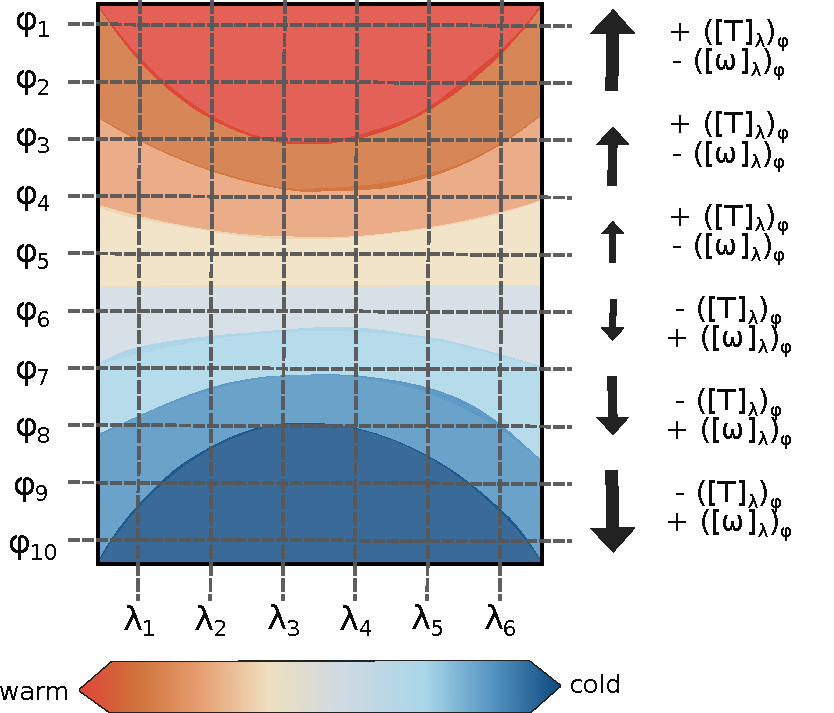
\includegraphics[width=0.75\columnwidth,angle=0]{fig/Cz.pdf}
\caption[$C_Z$ - representation]{Hypothetical situation illustrating the conversion term between available potential energy ($A_Z$) and kinetic energy ($K_Z$), represented by $C_Z$. The y-axis represents latitude circles ($\phi$), showing a decrease in temperature and vertical velocity $\omega$ (indicated by vertical arrows) toward the pole in the Southern Hemisphere. The x-axis represents longitude ($\lambda$).}
\label{Cz}
\end{center}
\end{figure}

% CA

The term $C_A$ (Equation \ref{eq:CA}) describes the energy conversion between zonal mean available potential energy ($A_Z$) and eddy available potential energy ($A_E$). Positive values of $C_A$ signify energy transfer from $A_Z$ to $A_E$, whereas negative values indicate the opposite. The equation for $C_A$ can be divided into two components, each capturing how deviations from the zonal mean of the meridional (north-south) and vertical winds (addressed in the first and second components, respectively) interact with latitudinal temperature gradients.

In the first component, we have $(v)_\lambda (T)_\lambda \frac{\partial ([T]_\lambda)\varphi}{\partial \varphi}$. The negative sign within the equation implies that for $C_A$ to be positive, this term must be negative. To understand each term's contribution to the sign of $C_A$, consider an illustrative case: a midlatitude low-pressure system in the Southern Hemisphere with a cold front propagating west to the system and a warm front east (Figure \ref{fig:Ca}. In the cold front region, $(v)_\lambda$ is positive (northward), $(T)_\lambda$ is negative (cooler), and $\frac{\partial ([T]\lambda)\varphi}{\partial \varphi}$ is positive (temperature increases equator-ward). Conversely, in the warm front region, $(v)_\lambda$ is negative (southward), $(T)_\lambda$ is positive (warmer), and $\frac{\partial ([T]_\lambda)_\varphi}{\partial \varphi}$ remains positive. This configuration is consistent across both hemispheres when accounting for the appropriate directional changes in wind and temperature gradient.

\begin{figure}[h]
\begin{center}
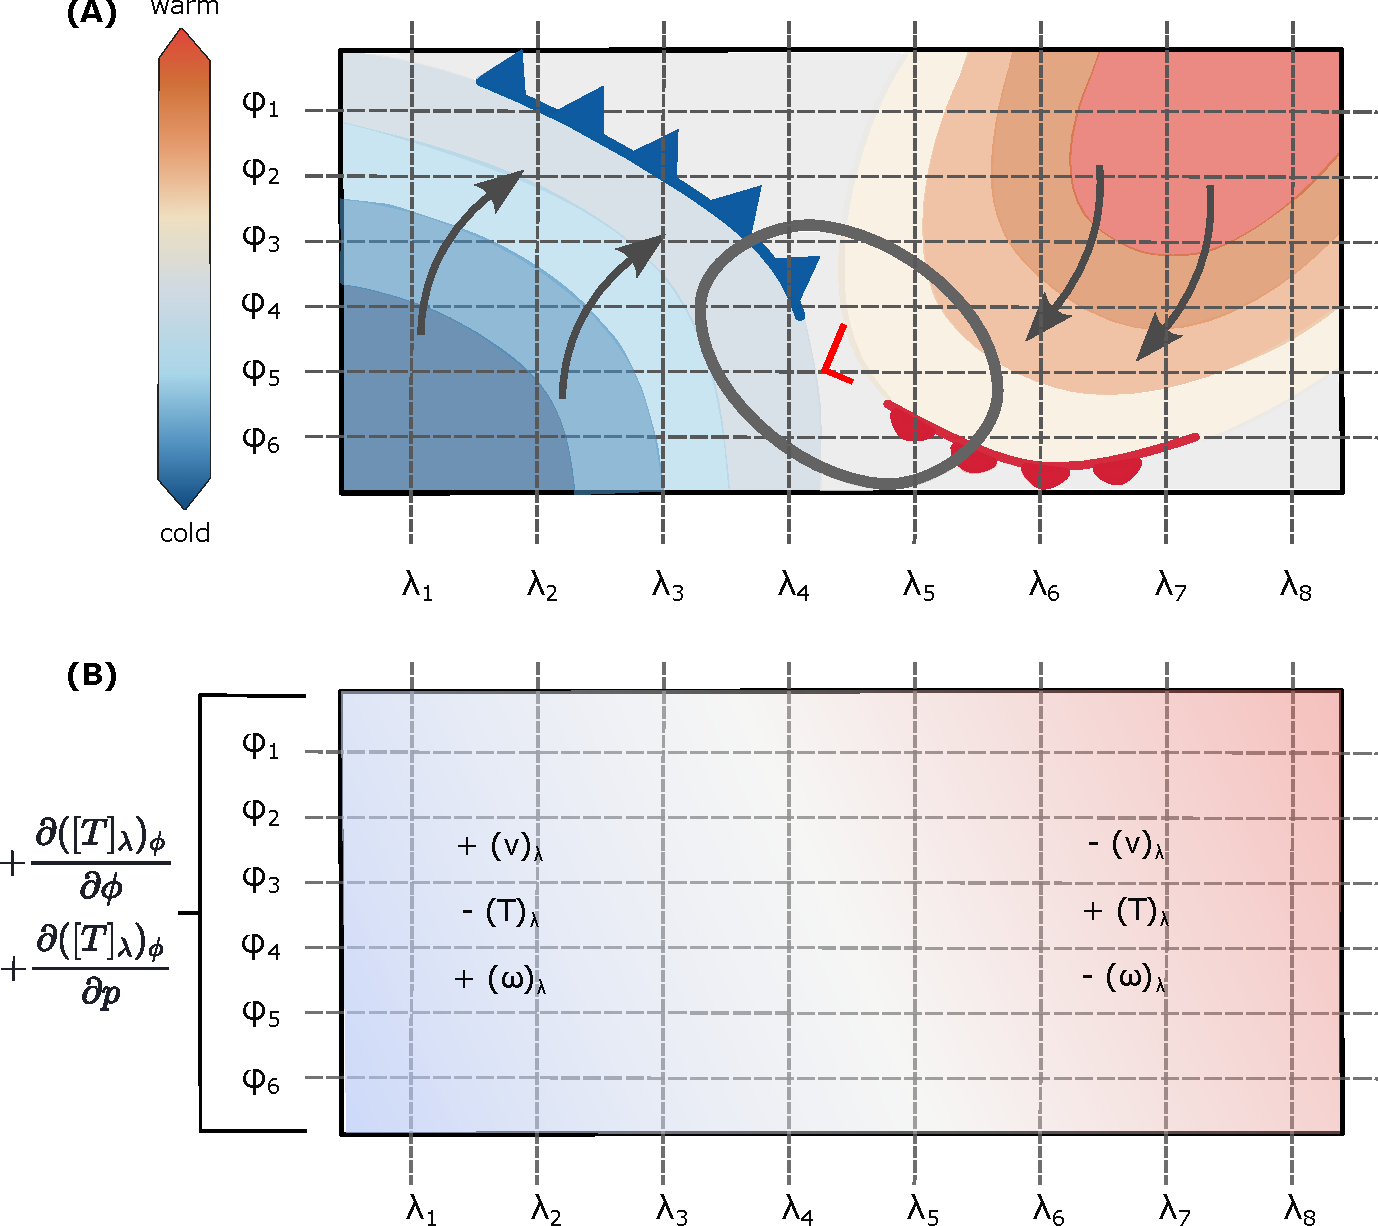
\includegraphics[width=0.8\textwidth]{fig/Ca.pdf}
\caption[$C_A$ - representation]{Representation of the conversion process between $A_Z$ and $A_E$. (A) Illustration of an idealized situation of a midlatitude low-pressure system in the Southern Hemisphere, with a cold front propagating west and a warm front east. (B) Analysis of the variables involved in the formula for $C_A$ (Equation \ref{eq:CA}). The y-axis represents latitude circles ($\phi$), and the x-axis represents longitude ($\lambda$). In the Southern Hemisphere, latitude decreases from $\phi_1$ to $\phi_6$.}
\label{fig:Ca}
\end{center}
\end{figure}

The second component, $(\omega)\lambda (T)\lambda \frac{\partial ([T]\lambda)\varphi}{\partial p}$, must also be negative to contribute positively to $C_A$. The term $\frac{\partial ([T]\lambda)\varphi}{\partial p}$ reflects the zonal average atmospheric lapse rate, which typically presents as negative over the cold air mass between $\phi_3$ and $\phi_6$ and between $\lambda_1$ and $\lambda_3$, indicating an increase in temperature with height. Above this level, the lapse rate reverses. In contrast, across the rest of the domain, particularly behind the warm front, this lapse rate term is positive. Consequently, when averaged across the domain and integrated over vertical levels, the overall contribution of this term tends to be positive. Furthermore, in the area behind the warm front, where $(\omega)\lambda$ is negative (indicating ascending air) and $(T)\lambda$ is positive (indicating warmer air), the product $(\omega)\lambda (T)\lambda$ is negative. This, in turn, results in a positive contribution to $C_A$, aligning with the term's requirement for a negative input to yield a positive output.

This analysis shows how an extratropical cyclone can influence global energetics. By transforming meridional into zonal temperature gradients, $C_A$ converts zonal APE into eddy APE. The described scenarios are generalizations and do not capture all atmospheric variations during frontal passages; however, they do reflect significant energetic contributions, especially at lower atmospheric levels. Additionally, it is important to note that the signs of the first and second components of $C_A$ do not need to match; $C_A$ will be positive if the magnitude of the negative component exceeds that of the positive component.

% CK

The last conversion term, $C_K$ (Equation \ref{eq:CK}), represents the conversion of kinetic energy from eddies to the zonal mean state. Positive values indicate an energy transfer from $K_E$ (eddy kinetic energy) to $K_Z$ (zonal kinetic energy), and vice versa. This term's formulation is more complex than others, comprising five distinct components: 1) meridional advection of zonal momentum, 2) meridional shear of meridional wind, 3) interaction of eddy zonal wind with zonal meridional wind, 4) vertical advection of zonal momentum, and 5) vertical advection of meridional momentum.

For simplicity, in analyzing the first term—meridional advection of zonal momentum—we consider \( (u)_\lambda \), \( (v)_\lambda \), and \( \frac{\partial [u]_\lambda}{\partial \phi} \), omitting variables related to the transformation from Cartesian to spherical coordinates. Consider a purely zonal westerly jet (Figure \ref{fig:Ck_1}a), where as latitude decreases from \( \phi_1 \) to \( \phi_{10} \), \( \frac{\partial [u]_\lambda}{\partial \phi} \) transitions from negative in the northern part of the domain to positive in the southern part. However, both \( v \) and \( (u)_\lambda \) are null in this scenario. Similarly, for a purely meridional northerly jet (Figure \ref{fig:Ck_1}b), \( (v)_\lambda \) varies from negative to positive across the domain, but \( (u)_\lambda \) and \( \frac{\partial [u]_\lambda}{\partial \phi} \) remain null. Therefore, averaged over the entire domain, this term is null for both scenarios.

\begin{figure}[h]
\begin{center}
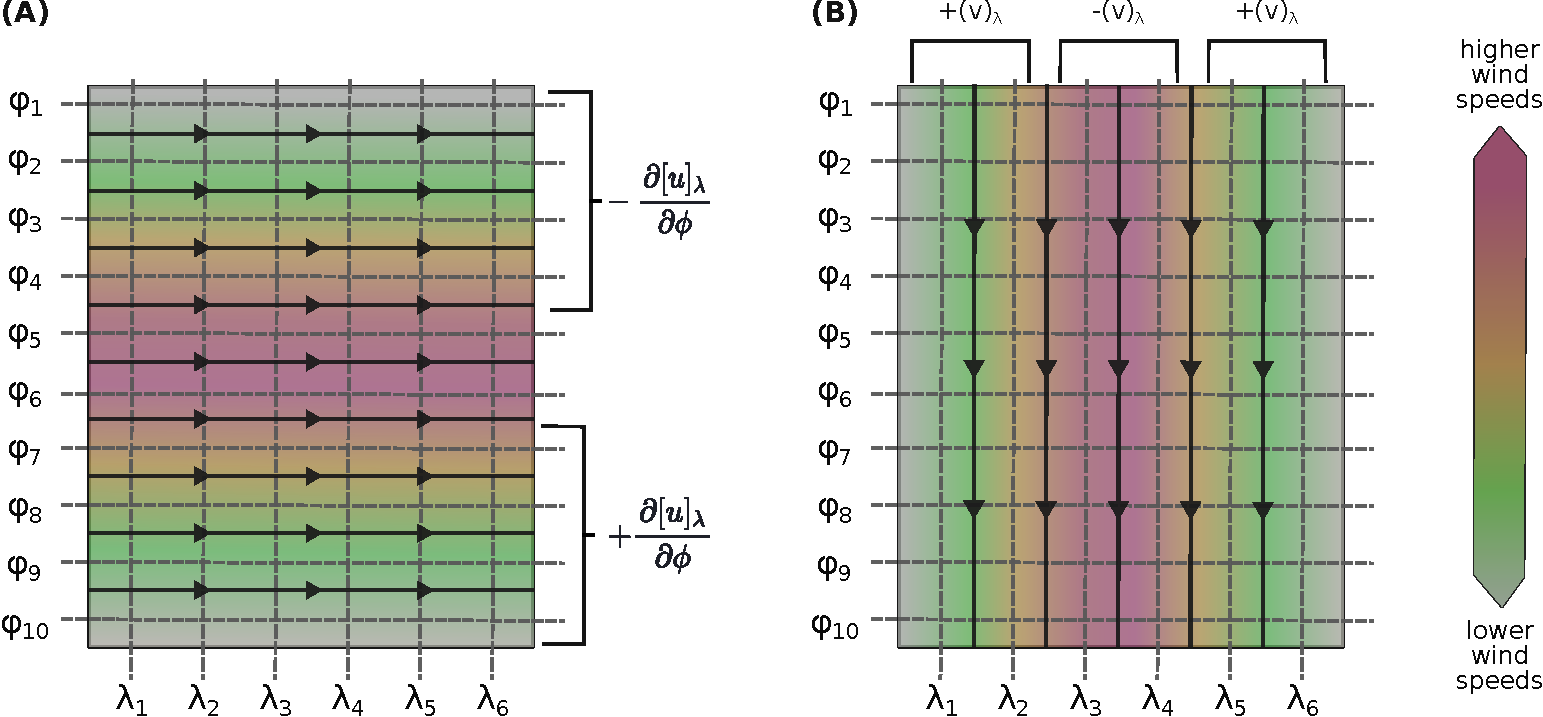
\includegraphics[width=0.8\textwidth]{fig/Ck_1.pdf}
\caption[Zonal and meridional jets]{Illustration of (A) a zonal westerly jet and (B) a meridional northerly jet in the Southern Hemisphere. The y-axis represents the latitude circles (\(\phi\)) and the x-axis represents longitude (\(\lambda\)).}
\label{fig:Ck_1}
\end{center}
\end{figure}

In situations where small instabilities arise in the zonal or meridional flow, they may initiate the development of larger instabilities. For example, consider a zonal jet becoming unstable with a cyclonic (clockwise) deviation in its flow at the southern part of the domain (Figure \ref{fig:Ck_2}a). Similarly as in a purely zonal jet, \( \frac{\partial [u]_\lambda}{\partial \phi} \) exhibits negative values in the northern part of the domain and positive values in the southern part (Figure \ref{fig:Ck_2}b). With the onset of instability, \( (v)_\lambda \) and \( (u)_\lambda \) are no longer null across the domain: they are negative on the eastern flank and positive on the western flank of the perturbation. This leads to a positive contribution to \( C_K \) from the first term, indicating that the eddy is transferring energy to the zonal flow and thus depleting its own energy over time.

\begin{figure}[h]
\begin{center}
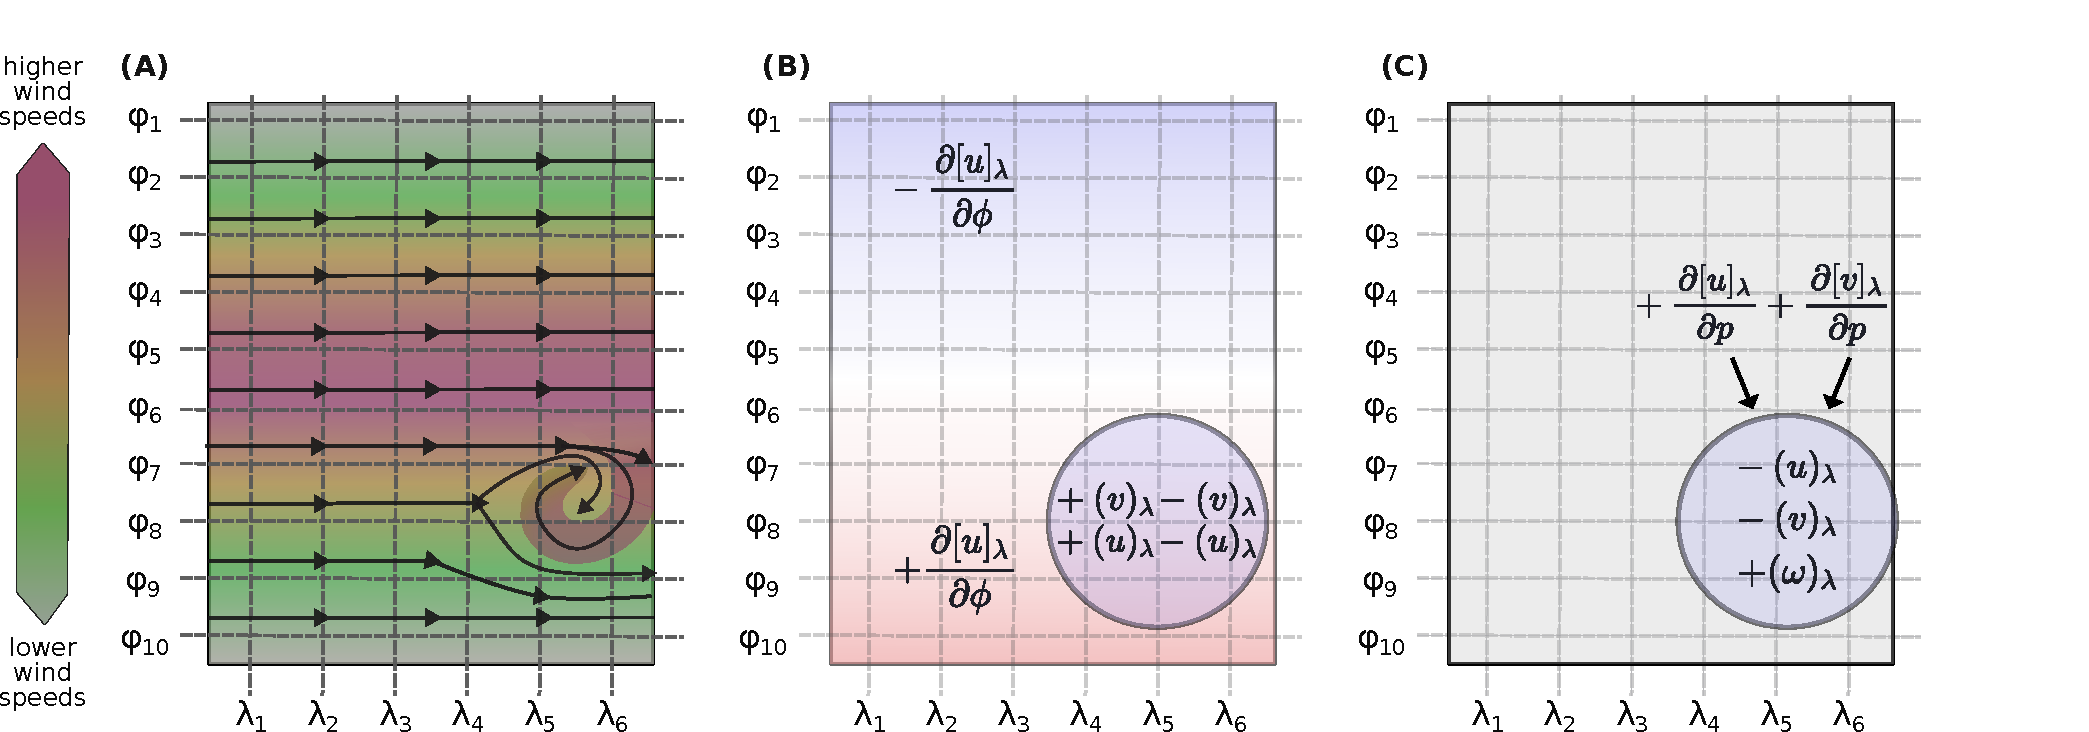
\includegraphics[width=0.9\textwidth]{fig/Ck_2.pdf}
\caption[Meridional jet - eddy]{(A) Illustration of an eddy developing in the southern part of a purely meridional jet, (B) signal analysis for the first, (C) fourth and fifth terms of \( C_K \) (Equation \ref{eq:CK}), for this scenario. The y-axis represents the latitude circles (\(\phi\)) and the x-axis represents longitude (\(\lambda\)).}
\label{fig:Ck_2}
\end{center}
\end{figure}

The second term in \( C_K \) - meridional shear of meridional wind - contains \( (v)^{2}_\lambda \frac{\partial [v]_\lambda}{\partial \phi} \). It is evident that \( (v)^{2}_\lambda \) is null for purely zonal jets, but otherwise is always positive, hence \( \frac{\partial [v]_\lambda}{\partial \phi} \) dictates this term's contribution to the signal of \( C_K \). While \( \frac{\partial [v]_\lambda}{\partial \phi} \) is typically null for purely zonal and meridional jets, its contribution becomes significant for small instabilities in the zonal flow. For the eddy development illustrated in Figure \ref{fig:Ck_2}a, as \( |v| \) decreases from the western to the eastern flank of the perturbation, \( [u] < 0 \), so \( \frac{\partial [v]_\lambda}{\partial \phi} > 0 \), making this term's contribution to \( C_K \) positive.

The third term - interaction of eddy zonal wind with zonal meridional wind - contains \( (u)^{2}_\lambda [v]_\lambda \). Both \( (u)^{2}_\lambda \) and \( [v]_\lambda \) are null for purely zonal jets. However, similar to the previous terms, their combined signal can be investigated for perturbations in the zonal flow. As \( (u)^{2}_\lambda \) is invariably positive, the signal of this term is influenced by \( [v]_\lambda \). In the situation depicted in Figure \ref{fig:Ck_2}a, \( [v]_\lambda < 0 \) leads to a negative contribution of this term to \( C_K \).

For the fourth and fifth terms - vertical advection of zonal and meridional momentum, respectively - the analysis is more complex due to the three-dimensional variations in wind throughout the troposphere. The fourth term involves \( (\omega)_\lambda (u)_\lambda \frac{\partial [u]_\lambda}{\partial p} \), while the fifth includes \( (\omega)_\lambda (v)_\lambda \frac{\partial [v]_\lambda}{\partial p} \). In scenarios of purely zonal jets, both terms are null, but they become significant with perturbations in the zonal flow.

Specifically, at mid-latitudes, we can assume that \( \frac{\partial [u]_\lambda}{\partial p} \) is generally negative (\([u]\) increases with height) in the troposphere. However, in the scenario illustrated in Figure \ref{fig:Ck_2}a, where the flow intensifies on the eastern flank of a perturbation, \( [u]_\lambda \) becomes negative (westward), making \( \frac{\partial [u]_\lambda}{\partial p} > 0 \) (Figure \ref{fig:Ck_2}c). Additionally, if the jet is at a higher altitude (e.g., 250 hPa), the convergence caused by the perturbation results in descending air, thus \( (\omega)_\lambda \) is positive. These conditions render the contribution of this term to \( C_K \) negative. The analysis for the fifth term follows similarly, where \( \frac{\partial [v]_\lambda}{\partial p} > 0 \), \( (u)_\lambda > 0 \), and \( (\omega)_\lambda > 0 \) (Figure \ref{fig:Ck_2}c), resulting in a negative contribution for this term to \( C_K \).

Collectively, the first two terms contribute positively to \( C_K \) while the last three terms provide negative contributions. Thus, the terms that, when summed, present the highest magnitude, will dictate the overall signal for \( C_K \). It is essential to recognize that the illustrative examples provided - zonal and meridional flows and a perturbation developing in the zonal flow - are simplifications of atmospheric motion. They are not intended to present a comprehensive picture of all conditions under which conversion between \( K_Z \) and \( K_E \) might occur but serve as guiding thought experiments to aid understanding of this conversion in real atmospheric motions. To the author's knowledge, due to the complexity of such analysis, no comprehensive attempt has been made previously in the literature.


The APE generation and K dissipation terms are defined as:

\begin{align}
    &G_Z =  \int_{p_t}^{p_b} \frac{[([q]_\lambda)_\phi ([T]_\lambda)_\phi]_{\lambda \phi}}{c_p[\sigma]_{\lambda \phi}} dp \\
    &G_E =  \int_{p_t}^{p_b} \frac{[(q)_\lambda (T)_\lambda]_{\lambda \phi}}{c_p[\sigma]_{\lambda \phi}} dp \\
    &D_Z = -  \int_{p_t}^{p_b} \frac{1}{g} [[u]_\lambda [F_\lambda]_\lambda + [v]_\lambda [F_\phi]_\lambda]_{\lambda \phi} dp \\
    &D_E = -  \int_{p_t}^{p_b} \frac{1}{g} [(u)_\lambda (F_\lambda)_\lambda + (v)_\lambda (F_\phi)_\lambda]_{\lambda \phi} dp
\end{align}

Here, $F_{\lambda}$ and $F_{\phi}$ represent the zonal and meridional frictional components, respectively, and $q$ is the diabatic heating term, computed as a residual from the thermodynamic equation:

\begin{equation}
    \frac{q}{c_p} = \frac{\partial T}{\partial t} + \Vec{V}_H \cdot \Vec{\nabla}_p T - S_p\omega
\end{equation}

where $\Vec{V}_H \cdot \Vec{\nabla}_p T$ represents the horizontal advection of temperature and $S_p$ approximates the static stability, given by:

\begin{equation}
    S_p \equiv -\frac{T}{\theta}\frac{\partial \theta}{\partial p}
\end{equation}

where $\theta$ is the potential temperature. 

The terms \( G_Z \) and \( G_E \) functionally resemble \( A_Z \) and \( A_E \), respectively. The variable \( q \) quantifies the heat added to or removed from an air parcel through external sources such as radiation, latent heat release (e.g., condensation), and sensible heat exchange (e.g., conduction from the surface). The variable \( \sigma \) represents the overall stratification of the atmosphere. Generation of \( G_Z \) or \( G_E \) occurs when anomalous heating aligns with regions of anomalously high temperature, and anomalous cooling coincides with regions of anomalously low temperature. If the temperature/heating gradients are meridional (e.g., differential heating from the equator to the poles), \( G_Z \) is generated. Conversely, if the gradients are within the same latitude belt (e.g., differential heating between ocean and land), \( G_E \) is generated. Additionally, higher static stability, indicating a more stratified atmosphere, reduces the efficiency of APE generation, while lower static stability enhances it. Maximum generation of APE is analogous to the situation illustrated in Figure \ref{fig:Ca}.

The terms \( D_Z \) and \( D_E \) represent the dissipation of kinetic energy from the zonal mean state and the eddies, respectively. The variable \( F \) denotes the frictional forces acting on the wind, which includes elements such as surface drag and turbulent friction. These frictional forces, notably surface drag and turbulent friction within the boundary layer, oppose the wind direction, causing a reduction in wind speed and consequently dissipating kinetic energy. Additionally, \( D_Z \) and \( D_E \) can also represent energy exchanges between different scales, specifically the transfer of energy from the grid scale to the subgrid scale. These forces not only convert kinetic energy into thermal energy but also facilitate the transfer of energy to smaller scale motions, thereby contributing to the overall energy dissipation within the atmospheric system.


The boundary terms are given by:

\begin{align}
& \mathrm{BAZ}=c_1 \int_{p_1}^{p_2} \int_{\varphi_1}^{\varphi_2} \frac{1}{2[\sigma]_{\lambda_{\varphi}}}\left(2\left([T]_\lambda\right)_{\varphi}(T)_\lambda u+\left([T]_{\lambda_{\varphi}}\right)_{\varphi}^2 u\right)_{\lambda_1}^{\lambda_2} \nonumber \\
& \times d \varphi d p+c_2 \int_{p_1}^{p_2} \frac{1}{2[\sigma]_{\lambda \varphi}}\left(2\left[(v)_\lambda(T)_\lambda\right]_\lambda\left([T]_\lambda\right)_{\varphi} \cos \varphi \right. \left.+\left([T]_\lambda\right)_{\varphi}^2[v]_\lambda \cos \varphi\right)_{\varphi_1}^{\varphi_2} d p \nonumber \\
& -\frac{1}{2[\sigma]_{\lambda \varphi}}\left(\left[2(\omega)_\lambda(T)_\lambda\right]_\lambda\left([T]_\lambda\right)_{\varphi}+\left[[\omega]_\lambda\left([T]_\lambda\right)_{\varphi}^2\right]_{\lambda_{\varphi}}\right)_{p_1}^{p_2} \\
& \mathrm{BAE}=c_1 \int_{p_1}^{p_2} \int_{\varphi_1}^{\varphi_2} \frac{1}{2[\sigma]_{\lambda \varphi}}\left[u(T)_\lambda^2\right]_{\lambda_1}^{\lambda_2} d \varphi d p \nonumber \\
& +c_2 \int_{p_1}^{p_2} \frac{1}{2[\sigma]_{\lambda \varphi}}\left(\left[(T)_\lambda^2 v\right]_\lambda \cos \varphi\right)_{\varphi_1}^{^{\varphi_2}} d p \\
& -\left(\frac{\left[\omega(T)_\lambda^2\right]_{\lambda \varphi}}{2[\sigma]_{\lambda \varphi}}\right)_{p_1}^{p_2} \nonumber \\
& \mathrm{BKZ}=c_1 \int_{p_1}^{p_2} \int_{\varphi_1}^{\varphi_2} \frac{1}{2 g}\left(u\left[u^2+v^2-(u)_\lambda^2-(v)_\lambda^2\right]\right)_{\lambda_1}^{\lambda_2} \nonumber \\
& \times d \varphi d p+c_2 \int_{p_1}^{p_2} \frac{1}{2 g}\left(\left[v \cos \varphi \left[u^2+v^2\right.\right.\right. \left.\left.-(u)_\lambda^2-(v)_\lambda^2\right]\right]_{\varphi_1}^{\varphi_2} d p  \\
& -\left(\frac{1}{2 g}\left[\omega\left[u^2+v^2-(u)_\lambda^2-(v)_\lambda^2\right]\right]_{\lambda \varphi}\right)_{p_1}^{p_2} \nonumber \\
& \mathrm{BKE}=c_1 \int_{p_1}^{p_2} \int_{\varphi_1}^{\varphi_2} \frac{1}{2 g}\left(u\left[(u)_\lambda^2+(v)_\lambda^2\right]\right)_{\lambda_1}^{\lambda_2} d \varphi d p \nonumber \\
& +c_2 \int_{p_1}^{p_2} \frac{1}{2 g}\left(\left[v \cos \varphi\left[(u)_\lambda^2+(v)_\lambda^2\right]\right]_\lambda\right)_{\varphi_1}^{\varphi_2} d p \\
& -\left(\frac{1}{2 g}\left[\omega\left[(u)_\lambda^2+(v)_\lambda^2\right]\right]_{\lambda \varphi}\right)_{p_1}^{p_2} \nonumber
\end{align}

where $c_1=-\left[a\left(\lambda_2-\lambda_1\right)\left(\sin \varphi_2-\sin \varphi_1\right)\right]^{-1}, c_2=-[a$ $\left.x\left(\sin \varphi_2-\sin \varphi_1\right)\right]^{-1}$.

The boundary terms \(BA_Z\), \(BA_E\), \(BK_Z\), and \(BK_E\) represent the fluxes of \(A_Z\), \(A_E\), \(K_Z\), and \(K_E\), respectively, from the lateral and vertical boundaries. Each boundary term has three components and shares a similar structure. For exemplification purposes, let's look into the \(BA_Z\) term. The first component represents the contribution of the zonal temperature flux anomalies to the \(A_Z\) term at the western and eastern boundaries. This term is computed for the westernmost and easternmost longitudes, integrated over all latitudes and pressure levels, and averaged over the entire domain. The second component is similar to the first one, representing the contribution of the meridional temperature flux anomalies to the \(A_Z\) term at the southern and northern boundaries. This term is computed for the southernmost and northernmost latitudes, integrated over all longitudes and pressure levels, and averaged over the entire domain. The third component represents the contribution of the vertical temperature flux anomalies to the \(A_Z\) term at the top and bottom boundaries. This term is computed for the topmost and bottommost pressure levels, integrated over all longitudes and latitudes, and averaged over the entire domain. The same logic can be applied to all other terms, substituting \(A_Z\) with \(A_E\), \(K_Z\), and \(K_E\), respectively.

The boundary terms \(BA_Z\), \(BA_E\), \(BK_Z\), and \(BK_E\) represent the fluxes of \(A_Z\), \(A_E\), \(K_Z\), and \(K_E\), respectively, from the lateral and vertical boundaries. Each boundary term includes three components, all sharing a similar structure. To exemplify, consider the \(BA_Z\) term. The first component quantifies the contribution of zonal temperature flux anomalies to the \(A_Z\) term at the western and eastern boundaries. This term is calculated for the westernmost and easternmost longitudes, integrated over all latitudes and pressure levels, and averaged over the entire domain. The second component mirrors the first, representing the contribution of meridional temperature flux anomalies to the \(A_Z\) term at the southern and northern boundaries. This term is evaluated for the southernmost and northernmost latitudes, integrated across all pressure levels, and averaged domain-wide. The third component accounts for the contribution of vertical temperature flux anomalies to the \(A_Z\) term at the top and bottom boundaries. This term is calculated at the topmost and bottommost pressure levels and similarly averaged over the entire domain. Applying the same logic, the \(BA_E\), \(BK_Z\), and \(BK_E\) terms are structured analogously, with adjustments to the specific energetic terms they represent—substituting \(A_Z\) with \(A_E\), \(K_Z\), and \(K_E\) respectively.

Lastly, the terms $B\Phi Z$ and $B\Phi E$ are given by:

\begin{align}
\mathrm{B} \Phi \mathrm{Z}= & c_1 \int_{p_1}^{p_2} \int_{\varphi_1}^{\varphi_2} \frac{1}{g}\left([v]_\lambda\left([\Phi]_\lambda\right)_{\varphi}\right)_{\lambda_1}^{\lambda_2} d \varphi d p \nonumber \\
& +c_2 \int_{p_1}^{p_2} \frac{1}{g}\left(\cos \varphi[v]_\lambda\left([\Phi]_\lambda\right)_{\varphi}\right)_{\varphi_1}^{\varphi_2} d p  \\
& -\frac{1} {g}\left(\left[\left([\omega]_\lambda\right)_{\varphi}\left([\Phi]_\lambda\right)_{\varphi}\right]_{\lambda_{\varphi}}\right)_{p_1}^{p_2} \nonumber \\
\mathrm{~B} \Phi \mathrm{E}= & c_1 \int_{p_1}^{p_2} \int_{\varphi_1}^{\varphi_2} \frac{1}{g}\left((u)_\lambda(\Phi)_{\lambda_\lambda}\right)_{\lambda_1}^{\lambda_2} d \varphi d p \nonumber \\
& +c_2 \int_{p_1}^{p_2} \frac{1}{g}\left(\left[(v)_\lambda(\Phi)_{\lambda_\lambda}\right]_\lambda \cos \varphi\right)_{\varphi_1}^{\varphi_2} d p \\
& -\frac{1}{g}\left(\left[(\omega)_\lambda(\Phi)_\lambda\right]_{\lambda_{\varphi}}\right)_{p_1}^{p_2} \nonumber
\end{align}

The terms \(B\Phi Z\) and \(B\Phi E\) describe the dynamical mechanisms that produce or destroy kinetic energy. As elucidated by \citet{muench1965dynamics}, these terms, along with \(C_Z\) and \(C_E\), involve a arise from the derivation of the term \(\Vec{V} \cdot \nabla \Phi\). This expression represents the generation of kinetic energy through cross-isobaric flow towards areas of low pressure. Conversely, the destruction of kinetic energy occurs when there is cross-isobaric flow towards areas of high pressure.


Apart from examining the individual contributions of each term to the energy cycle, the Lorenz Energy Cycle (LEC) highlights specific interactions between terms that elucidate distinct dynamical mechanisms (Figure \ref{fig:lec_chains}). The \(A_Z\) term, involving meridional gradients of temperature and atmospheric stability, interacts in such a way that \(C_A > 0\) acts to diminish these gradients through the meridional transport of sensible heat. This process sets the stage for \(C_E > 0\), driven by the zonal temperature gradient and vertical motions. In contrast, the conversion from \(K_Z\) to \(K_E\) (\(C_K\)) redistributes kinetic energy without altering the thermal structure and is primarily influenced by the horizontal shear of the mean flow. Therefore, the processes \(A_Z \rightarrow A_E \rightarrow K_E\) are often referred to as the "baroclinic chain," while \(C_K\) is known as the barotropic conversion term \citep[e.g.]{michaelides1992spatial, veiga2013global, pezza2014large, okajima2021cyclonic}. Additionally, the term "moist baroclinic chain" is used here to refer to the process where \(G_E\) supplies energy to \(A_E\), acting in consonance with the baroclinic chain.

\begin{figure}[h]
\centering
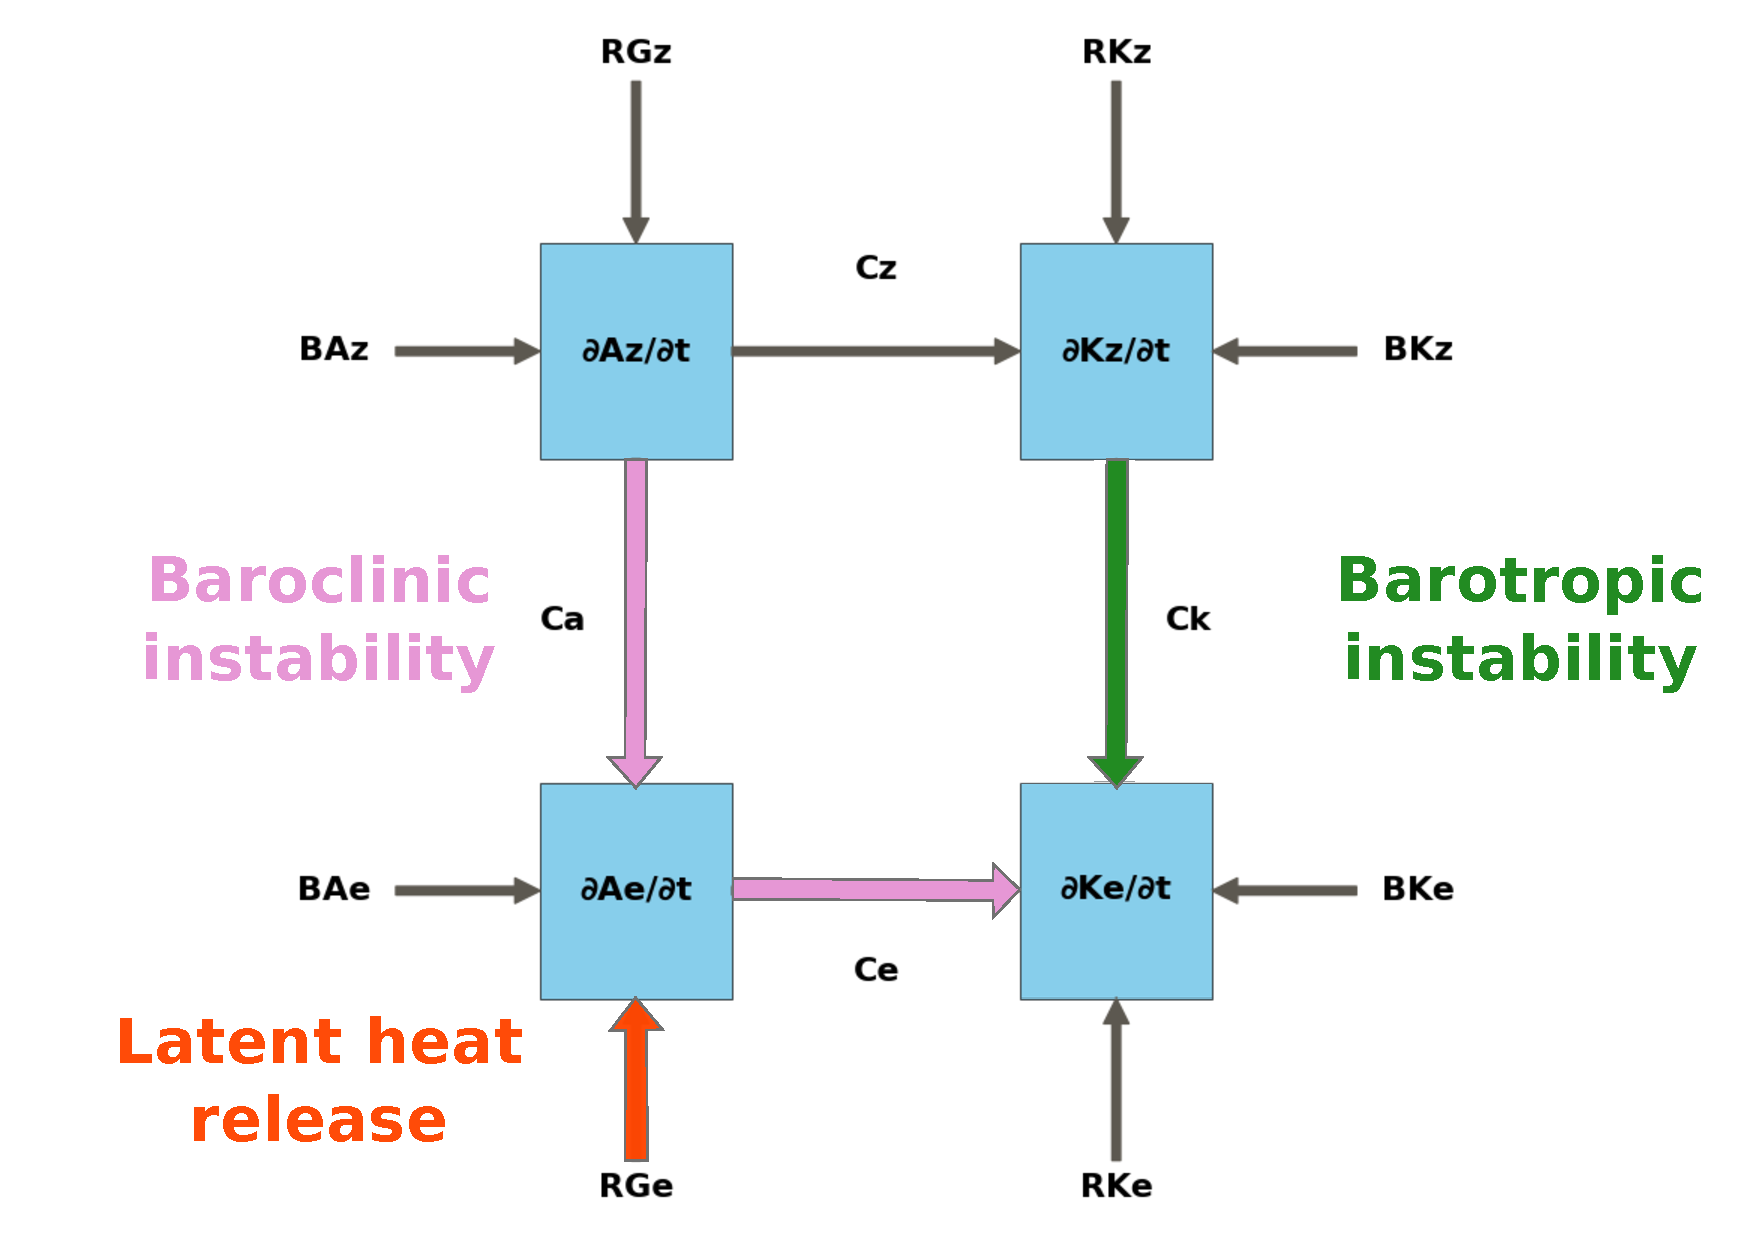
\includegraphics[width=\linewidth]{fig/LEC_chains.pdf}
\caption[LEC - chains]{Schematic representation of the different energy conversion chains in the Lorenz Energy Cycle. The diagram illustrates the "baroclinic chain" (\(A_Z \rightarrow A_E \rightarrow K_E\)), indicating the role of baroclinic instability, the contribution of latent heat release by the \(G_E\) term and the "barotropic chain" (\(K_Z \rightarrow K_E\)).}
\label{fig:lec_chains}
\end{figure}

\subsection{Lorenz Energy Cycle applied to cyclonic systems}

During the 1960s and 1970s, extensive research was conducted on the energetics of extratropical cyclonic systems. \citet{smith1980energetics} reviewed these studies, offering a detailed summary of their outcomes. According to the mean kinetic energy (K) budgets, cyclones are areas of relatively higher concentrated kinetic energy compared to the rest of the hemisphere, though the difference is not markedly substantial. Cyclones are characterized by significant energetic activity, with substantial $K_E$ generation through cross-contour flow. This generation is nearly balanced by the horizontal export of energy and its dissipation. Mature cyclones typically exhibit negative values for \(D_E\); however, in certain scenarios, \(D_E\) can act as an energy source (\(D_E > 0\)), especially in regions characterized by intense convection or the presence of short upper air waves, predominantly above the planetary boundary layer. This dynamic might be associated with energy transfer from sub-grid scales to the grid scale. Additionally, latent heat release from convective processes plays a critical role in the generation of APE in extratropical cyclones. Generally, cyclones are inefficient thermodynamic systems; a significant portion of \(A_E\) is not converted into \(K_E\), leading to an energy conversion efficiency of only 3\% to 4\%. Cyclones account for approximately 6\% of the hemispheric energy contribution. However, intense cyclones, which are about 50\% more energetically active than average, can contribute up to 20\% of the hemispheric energy. 

More recently, the study by \citet{black2013universal} provides a detailed climatology of the energetics of cyclonic systems, specifically focusing on explosive cyclones. This research spans four major regions—the Northwest Pacific, the North Atlantic, the Southwest Pacific, and the South Atlantic—utilizing a 32-year climatology to analyze these phenomena. The analysis reveals that anomalous energy conversions begin approximately 48 hours before the explosive cyclone development and remain strong for up to 120 hours. The results demonstrate that the baroclinic chain is the primary mechanism driving the energy dynamics during explosive cyclogenesis, and this holds true across different regions and times of the year. Furthermore, the study finds that within the analyzed domains, the energetic signatures of regular cyclones often merge with background noise, making them indistinguishable.

The review by \citet{smith1980energetics} provides a broad overview of the energy budget of extratropical cyclones, focusing primarily on their contributions to general circulation rather than on the dynamical mechanisms essential for their development, intensification, and decay. Meanwhile, \citet{black2013universal} offers a more detailed picture, especially of explosive cyclones. However, the difficulty in distinguishing the energetic signatures of regular cyclones from background noise may be attributed to the large computational domains used, which are extensive enough to include multiple cyclonic systems simultaneously, potentially complicating the analysis. To overcome these challenges and gain a deeper understanding of cyclonic energetics, specific case studies are essential. These studies provide insights into how various energy transformations within a cyclone contribute to its lifecycle. The literature reviewed in the next paragraphs highlights the pathways that supply energy to the eddy energy reservoirs, with particular emphasis on the \(K_E\) term, which serves as a proxy for the system's intensity. Special attention is given to the contributions of the baroclinic (\(A_Z \rightarrow A_E \rightarrow K_E\)) and barotropic (\(K_Z \rightarrow K_E\)) chains, as well as to the contributions from latent heat release (\(G_E\)) due to the eddy's convective activity. These elements are crucial for understanding the energetic dynamics that drive cyclone behavior and evolution.

% Tropical

There are only a few studies accessing the Lorenz Energy Cycle in the context of tropical cyclones. For instance, \citet{brennan1980zonal} analyzes the synoptic-scale energy budget of Hurricane Carmen (1979) as it intensified from a tropical depression to a major hurricane. During the tropical depression stage, \(K_E\) serves as a source of energy for both \(A_E\) and \(K_Z\), while also exporting energy (\(BK_E < 0\)), primarily sustained by \(RK_E\). Concurrently, \(A_E\) exports energy (\(BA_E < 0\)) and experiences energy destruction due to diabatic cooling and/or descending movements (\(G_E < 0\)). This suggests that during this phase, the system predominantly relies on up-scaling of energy from subgrid scales and/or cross-isobaric flow (\(B\Phi E > 0\)). However, during the hurricane stage, diabatic heating (from \(G_E\)) begins to supply energy to \(A_E\), further supported by the import of energy (\(BA_E > 0\)) and conversion from \(A_Z\). Most of this energy is transformed into \(K_E\). Additionally, the zonal circulation contributes to the eddy energy (\(C_K < 0\)). Consequently, during the hurricane phase, moist baroclinic processes drive the system's development, supplemented by barotropic conversions. Despite an overall reduction in \(K_E\) and \(K_Z\), the storm's circulation intensifies. The author attributes this paradox to mesoscale processes not being adequately resolved due to the poor resolution of the dataset, with negative values for both \(D_Z\) and \(D_E\) indicating an energy transfer from the resolved synoptic scale to the mesoscale. These observations imply that higher resolution datasets might reveal different dynamics for \(K_E\) and \(K_Z\) budgets.

Although the study by \citet{brennan1980zonal} provided important insights into the environmental energetics changes during hurricane formation, several caveats merit discussion. First, the dataset used features a coarse resolution with \(2.5^\circ\) grid spacing, which is insufficient to accurately represent mesoscale phenomena associated with the hurricane. Additionally, the data consisted primarily of point-source rawinsonde observations, surface observations, and daily infrared satellite imagery, with gaps filled by linear interpolation. Lastly, the computational domain was excessively large (\(50^\circ \times 50^\circ\)), raising concerns that the system's energetics could be confounded with background environmental influences. These limitations suggest that the study's findings should be interpreted with caution, considering the potential blending of cyclone energetics with broader atmospheric processes.

Using data from the NCEP/NCAR reanalysis, \citet{veiga2008analysis} analyzed the energy budget for Hurricane Catarina, distinguishing its development into distinct phases. During the extra-tropical phase, the moist baroclinic chain was active, with both \(A_Z\) and \(G_E\) supplying energy to \(A_E\), which was predominantly converted into \(K_E\). As the system transitioned into the tropical phase, this chain loss intensity, notably as \(G_E\) decreased significantly, making the conversion from \(K_Z\) to \(K_E\) the primary contributor to \(K_E\). However, much of this energy was exported from the domain, leading to a decrease in \(K_E\). Upon reaching Category 1 Hurricane status, there was a reversal in the sign of the baroclinic chain, characterized by conversions from \(K_E\) to \(A_E\) to \(A_Z\), with both \(C_K\) and \(RK_E\) playing roles in augmenting \(K_E\). 

 % Subtropical 
 
More attention was given to the energetics of subtropical cyclones than to the tropical systems. \citet{michaelides1987limited} analyzes the synoptic-scale energy budget of a frontal depression that initially formed in the Mediterranean region, categorizing its evolution into four distinct phases. Although the nomenclature was not established at the time, the system might potentially have been classified as a medicane, a type of subtropical cyclone that originates in the Mediterranean \citep{da2019subtropical}. During the precyclogenetic period ("incipient stage"), \(A_E\) is sustained by contributions from \(A_Z\), \(K_E\), and \(BA_E\). However, it experiences a net decrease due to negative generation from cooling and descending motions. Meanwhile, \(K_E\) sees an increase, fueled by conversions from \(K_Z\) and energy import. As cyclogenesis begins ("intensification stage"), the signals for both \(C_A\) and \(C_E\) reverse, enabling \(A_E\) to feed both \(A_Z\) and \(K_Z\), supported by energy import and positive \(G_E\). Although \(K_Z\) continues to enhance \(K_E\), increased dissipation begins to diminish \(K_E\). In the development phase ("mature phase"), \(A_E\) reaches its peak, primarily due to latent heat generation and significant energy import. \(A_E\) is actively converted to \(K_E\), yet \(K_E\) continues to decline overall, affected by heightened dissipation and energy conversions to \(K_Z\). In the post-cyclogenesis phase ("decay phase"), both \(A_E\) and \(K_E\) diminish as the system weakens, with marked reductions in import, conversion rates, and \(D_E\) reaching its maximum.

In their study, \citet{dias2013synoptic} investigate the potential for tropical transition of Subtropical Cyclone Anita near the southeast Brazilian coast. During the early stages of the system, the barotropic chain primarily fueled \(K_E\). As the system evolved into a hybrid stage and approached its potential for tropical transition, both moist baroclinic and barotropic chains actively supplied energy to \(K_E\), complemented by positive values of \(G_E\) due to convective processes. Concurrently, the system exported both \(A_E\) and \(K_E\) through its boundaries. Eventually, Anita entered a baroclinic environment and transitioned to an extratropical system. This phase was marked by a reversal in the sign of \(C_K\) and a dominance of the baroclinic chain in its energetics.

The study by \citet{pezza2014large} explores the energetics of the hybrid subtropical cyclone known as "Duck," which occurred over the Tasman Sea. Influenced by a persistent mid-latitude blocking high, the genesis of Duck created a conducive environment for cyclogenesis, with the system undergoing a partial tropical transition. During the genesis phase, a significant peak in \(C_K\) was observed, reaching a maximum near 350 hPa, facilitated by the presence of the blocking system — a similar environmental condition to that observed during Catarina's tropical transition. As Duck evolved, a secondary peak in baroclinic conversion coincided with the development of an upper-level warm core for the first time. However, the energy supply for $K_E$ during this stage was insufficient for a full tropical transition. The authors speculate that the baroclinic conversion prevented Duck from achieving a complete tropical transition, hence not reaching hurricane status.

The energetics of the Duck storm were also investigated by \citet{cavicchia2018energetics}, with comparisons made to an extratropical cyclone, the Pasha Bulker storm. Similar to findings by \citet{pezza2014large}, the Duck storm's lifecycle was predominantly influenced by the barotropic chain, which was the main source of energy for \(K_E\). In contrast, the Pasha Bulker storm was primarily driven by the baroclinic chain, with the most significant baroclinic energy conversions occurring during its intensification phase. However, \citet{cavicchia2018energetics} does not present results for generation and boundary terms, which limits the depth of the analysis.

% Mediterran

For extratropical cyclones, a larger body of literature exploring their energy cycle can be found, especially for the Mediterranean and South Atlantic regions. For instance, in \citet{michaelides1992spatial}, an extratropical system originating in the Mediterranean region is analyzed, providing a basis for comparison with the earlier study by \citet{michaelides1987limited}. During the initial development phase, \(A_E\) increases due to significant latent heat release and the advection of colder air over warmer waters, which enhances $G_E$ and $C_A$. Concurrently, \(K_E\) is sustained by conversions from both \(A_E\) and \(K_Z\). As cyclogenesis progresses, the energetic profile remains similar to the previous stage; however, convective activity and imports of \(A_E\) decline, leading to a decrease in this term. Simultaneously, an increase in \(D_E\) causes a reduction in the absolute value of \(K_E\). During this stage, \(K_E\) is primarily maintained by \(C_K\). In the mature phase, there is a further decline in \(G_E\) and imports of \(A_E\), causing \(A_E\) to decrease further. Additionally, as \(D_E\) increases and conversion from other terms decreases, \(K_E\) also diminishes over time. During the decay phase, \(G_E\) reaches its lowest level; however, \(A_E\) increases due to enhanced \(C_A\) and weakened \(C_E\). Conversely, \(K_E\), despite the weakened \(C_A\) and \(C_K\), increases as dissipation becomes minimal.

\citet{wahab2002mechanism} also analyzed the energy budget throughout the development of a Mediterranean cyclone. The cyclogenesis phase is characterized by a significant increase in \(K_E\), primarily supported by the residual term (\(RK_E\)), while \(A_E\) is initially sustained by \(K_E\). However, as the \(RG_E\) term increases, \(A_E\) begins to feed \(K_E\). The growth period of the cyclone is marked by \(K_E\) being bolstered by \(C_K\) and imports of energy, which are subsequently either dissipated or converted to \(A_E\), with \(RG_E\) acting as a sink of energy. During the dissipation period, \(A_E\) serves as a source of energy for both \(K_E\) and \(A_Z\). Concurrently, while \(K_E\) is supported by \(K_Z\) and imports of energy, dissipation acts as a significant sink of energy, resulting in a decrease in \(K_E\).

The study by \citet{bulic2006limited} investigates the energy budget associated with a deep and rapid cyclogenesis over the Mediterranean region, utilizing the ALADIN model. Before cyclogenesis, \(K_E\) is converted into \(A_E\), a process that reverses after the cyclone forms. Throughout the cyclone's lifecycle, \(C_K\) consistently supplies energy to \(K_E\). This conversion, most intense at upper levels around 350 hPa, is identified as crucial for the system's development. Additionally, \(B_{K_E}\) is responsible for exporting eddy energy throughout the entire lifecycle, except during the time of cyclone formation. The study highlights the cyclone's dependency on both baroclinic and barotropic processes; however, it also notes that the results may be limited to the dynamics captured by the model and might not fully reflect observational data.

% Extratropical

\citet{dias2011energy} analyzed the energy cycle for three extratropical cyclones, one for each genesis region in South America, detailing each system's development across formation, mature, and decay phases. For the first system, with genesis in the SE-BR region, the energetics were most active during the formation phase, where both baroclinic and barotropic chains provided energy to \(K_E\), with significant contributions from the \(C_K\) term. In the mature phase, the baroclinic chain reversed, making \(C_K\) the sole contributor to \(K_E\). During the decay phase, \(K_E\) transferred energy to \(K_Z\) and \(A_E\) to \(A_Z\). The second system, originating in the LA-PLATA region, maintained a consistent energy supply throughout its lifecycle via the moist baroclinic chain, most prominently during the mature phase. Throughout all phases, \(K_E\) consistently supplied energy to \(K_Z\). The third system, with its genesis in the ARG region, was primarily sustained by the baroclinic chain, with contributions from latent heat release (\(G_E\)) only during the mature phase. Although less significant, there was also an energy supply from \(C_K\) during the formation and mature phases.

The study by \citet{pezza2010environmental} examines the Lorenz energetics of a high-latitude baroclinic storm that caused severe flooding in Nome, Alaska. The trajectory and intensity of the storm were significantly influenced by a blocking high-pressure system that steered its path a week prior to its formation. From the onset of cyclogenesis to the rapid intensification phase, the environment transitioned from lower to higher energy states, marked by peaks in \(A_E\) and \(K_E\). During these phases, both the baroclinic and barotropic energy chains supplied energy to \(K_E\), with a smaller contribution from \(G_E\) to \(A_E\). The computational domain included the blocking region, highlighting the role of this high-pressure system in facilitating the energy conversion \(C_K\), which supplied \(K_E\) to the cyclonic system. As the storm reached its peak activity, the barotropic chain reversed, with \(K_E\) feeding energy back to zonal kinetic energy (\(K_Z\)). Thus, during this stage, the maintenance of the system was predominantly sustained by the baroclinic chain. Additionally, the peak in baroclinic energy transfer occurred approximately 18 hours before the storm reached maximum intensity, indicating significant preconditioning of the environment by the baroclinic processes.

% Differences in method

\citet{michaelides1999quasi} analyze the energetics of an intense Mediterranean cyclone, employing both Eulerian and quasi-Lagrangian frameworks for comparison. The quasi-Lagrangian framework reveals a significant increase in \(A_E\) during the cyclone's development, driven by diabatic heating processes such as latent heat release in the warm sector. Concurrently, \(K_E\) increases from the early stages to the maturity phase and then decreases as the cyclone decays. This initial rise in \(K_E\) is propelled by \(C_K\), especially prominent at the jet level in the upper troposphere. The transformations between \(A_E\) and \(K_E\) are characterized by initial conversions of \(A_E\) to \(K_E\), fueling the cyclone's intensification, followed by a reversal where \(K_E\) converts back to \(A_E\) as the system weakens. Notably, there are substantial imports of \(K_E\) during the cyclone's intensification phase and exports during its dissipation. The quasi-Lagrangian analysis indicates higher \(A_E\) and lower \(K_E\) compared to the Eulerian method, suggesting that the fixed volume method captures more ambient kinetic energy from surrounding regions. Both methods confirm an overall conversion from \(K_Z\) to \(K_E\), although the values are greater in the Eulerian method, and the conversions from \(A_E\) to \(K_E\) change signs. Additionally, there are reversals in signs for the boundary terms. The semi-Lagrangian method is considered to more genuinely represent the energetics characteristics of the synoptic system under study, as it isolates the cyclone as much as possible at all times. In contrast, the Eulerian method allows for circulations other than the cyclonic system under study to infringe into the computational region, potentially spuriously contaminating the cyclone's energetics.

The reviewed literature provides valuable insights into the energetics of different cyclonic systems. For tropical cyclones, although the limited body of literature prevents definitive conclusions, it appears that the barotropic chain, aided by the \(G_E\) term and subsequent conversions from \(A_E\) to \(K_E\), is a primary driver for cyclone development. This emphasis on barotropic instability aligns well with research highlighting the role of barotropic instability in tropical waves for the initial development of tropical cyclones, with further intensification facilitated by latent heat release \textit{via} CISK/WISHE mechanisms, as discussed in Section \ref{efficient_causes}. Meanwhile, studies on subtropical cyclones indicate a shared contribution from barotropic and baroclinic processes, with the moist contributions to the baroclinic chain being variably active. The barotropic chain seems particularly important in the initial stages, with the baroclinic chain gaining significance in later stages. For extratropical cyclones, contrary to expectations, the baroclinic chain is not the sole driver of their energy cycle; most case studies indicate a role for the barotropic chain in their development. From \citet{black2013universal}'s results, we can infer that the primary difference in the Lorenz Energy Cycle (LEC) between regular and explosive cyclones is the heightened importance of the baroclinic chain in the latter. Additionally, it is noteworthy that for both subtropical and extratropical systems, barotropic conversions occur predominantly at upper tropospheric levels. Nevertheless, while these energy pathways are crucial for system development, other terms also play important roles. For instance, \(D_E\) is often indicated as a significant sink for \(K_E\), with larger values as \(K_E\) increases. Additionally, imports of \(K_E\) (\(BK_E\)), particularly in the early stages of development, also contribute to system development.

From the reviewed literature, it is evident that the LEC methodology is a valuable diagnostic tool for studying cyclonic system dynamics. However, despite the methodology dating back to the 1960s and still being in use today, the body of literature on this topic is still expanding, primarily comprising case studies, with the only comprehensive climatology provided by \citet{black2013universal}. Furthermore, most case studies utilize the Eulerian framework, which may underestimate contributions from certain terms, as the large-scale environment might overshadow the systems' energetics. There is a need for more climatologies assessing the LEC for cyclonic systems—or at least analyses of a large number of systems—to better understand the energy pathways related to their development.
